% !TeX encoding = UTF-8
% !TeX root = master.tex
% !TeX spellcheck = en_US

\documentclass[11pt,a4paper,twoside,openright]{report}

\usepackage[utf8]{inputenc}
\usepackage[portuguese,english]{babel}
\selectlanguage{english}

\usepackage[mieic]{styles/feupteses}
% Additional options for feupteses.sty:
% - juri: prints line numbers
% - final: final version
% - onpaper: links are not shown (for paper versions)
% - backrefs: include back references from bibliography to citation place

%\usepackage[lofdepth,lotdepth]{subfig}
\usepackage{afterpage}
\usepackage{graphicx}
\usepackage{flafter}
\usepackage{animate}
\usepackage{float}
\usepackage{grffile}

\usepackage{color}
\definecolor{cloudwhite}{cmyk}{0,0,0,0.025}

\usepackage{listings}
\lstset{ %
 language=C++,                        % choose the language of the code
 basicstyle=\footnotesize\ttfamily,
 keywordstyle=\bfseries,
 numbers=left,                      % where to put the line-numbers
 numberstyle=\scriptsize\texttt,    % the size of the fonts that are used for the line-numbers
 stepnumber=1,                      % the step between two line-numbers. If it's 1 each line will be numbered
 numbersep=8pt,                     % how far the line-numbers are from the code
 frame=tb,
 float=htb,
 aboveskip=8mm,
 belowskip=4mm,
 backgroundcolor=\color{cloudwhite},
 showspaces=false,                  % show spaces adding particular underscores
 showstringspaces=false,            % underline spaces within strings
 showtabs=false,                    % show tabs within strings adding particular underscores
 tabsize=2,	                    % sets default tabsize to 2 spaces
 captionpos=b,                      % sets the caption-position to bottom
 breaklines=true,                   % sets automatic line breaking
 breakatwhitespace=false,           % sets if automatic breaks should only happen at whitespace
 escapeinside={\%*}{*)},            % if you want to add a comment within your code
 morekeywords={*,var,template,new}  % if you want to add more keywords to the set
}

\usepackage{amsmath}
\usepackage[algochapter,linesnumberedhidden]{algorithm2e}
\usepackage{booktabs}
\usepackage{tabu}
\usepackage{rotating}
\usepackage{array}
\usepackage{multirow}
\usepackage{easylist}
\usepackage{siunitx}
\usepackage{url}
\usepackage{caption}
\usepackage{subcaption} 
\usepackage{footnote}
\usepackage{footmisc}
\usepackage{hyperref}
\usepackage[all]{hypcap}
\usepackage[noabbrev,nameinlink]{cleveref}
\usepackage{etoolbox}
\usepackage[nonumberlist,acronym,xindy]{glossaries}

\usepackage{enumitem}
\setlist{nolistsep}

\graphicspath{{figures/}}
\setcounter{tocdepth}{3}

\makeglossaries
%\usepackage[xindy]{imakeidx}
%\makeindex


\newtoggle{showcommittee}
\toggletrue{showcommittee}

%some macro definitions

% format
\newcommand{\class}[1]{{\normalfont\slshape #1\/}}

% entities
\newcommand{\Feup}{Faculdade de Engenharia da Universidade do Porto}

% abbreviations:
\newacronym{agps}{AGPS}{Assisted Global Positioning System}
\newacronym{amcl}{AMCL}{Adaptive Monte Carlo Localization}
\newacronym{api}{API}{Application Programming Interface}
\newacronym{cad}{CAD}{Computer Aided Design}
\newacronym{carlos}{CARLoS}{Cooperative Autonomous Robot for Large Open Spaces}
\newacronym{dof}{DoF}{Degrees of Freedom}
\newacronym{dgps}{DGPS}{Differential Global Positioning System}
\newacronym{ekf}{EKF}{Extended Kalman Filter}
\newacronym{esf}{ESF}{Ensemble of Shape Functions}
\newacronym{fpfh}{FPFH}{Fast Point Feature Histogram}
\newacronym{glonass}{GLONASS}{GLObalnaya NAvigatsionnaya Sputnikovaya Sistema}
\newacronym{gnss}{GNSS}{Global Navigation Satellite System}
\newacronym{gps}{GPS}{Global Positioning System}
\newacronym{gpu}{GPU}{Graphics Processing Unit}
\newacronym{icp}{ICP}{Iterative Closest Point}
\newacronym{ip}{IP}{Internet Protocol}
\newacronym{iss3d}{ISS3D}{3D Intrinsic Shape Signatures}
\newacronym{lidar}{LIDAR}{LIght Detection And Ranging}
\newacronym{mcl}{MCL}{Monte Carlo Localization}
\newacronym{ndt}{NDT}{Normal Distributions Transform}
\newacronym{opencv}{OpenCV}{Open Computer Vision library}
\newacronym{openni}{OpenNI}{Open Natural Interaction library}
\newacronym{pca}{PCA}{Principal Component Analysis}
\newacronym{pcl}{PCL}{Point Cloud Library}
\newacronym{pfh}{PFH}{Point Feature Histogram}
\newacronym{radar}{RADAR}{RAdio Detection And Ranging}
\newacronym{ransac}{RANSAC}{Random Sample Consensus}
\newacronym{ros}{ROS}{Robot Operating System}
\newacronym{rmse}{RMSE}{Root Mean Square Error}
\newacronym{sacia}{SAC-IA}{Sample Consensus Initial Alignment}
\newacronym{sc3d}{SC3D}{Shape Context 3D}
\newacronym{shot}{SHOT}{Signature of Histograms of Orientations}
\newacronym{sift}{SIFT}{Scale Invariant Feature Transform}
\newacronym{slam}{SLAM}{Simultaneous Localization And Mapping}
\newacronym{sonar}{SONAR}{SOund Navigation And Ranging}
\newacronym{tcp}{TCP}{Transmission Control Protocol}
\newacronym{toa}{ToA}{Time of Arrival}
\newacronym{tof}{ToF}{Time of Flight}
\newacronym{ttff}{TTFF}{Time To First Fix}
\newacronym{udp}{UDP}{User Datagram Protocol}
\newacronym{ukf}{UKF}{Unscented Kalman Filter}
\newacronym{usc}{USC}{Unique Shape Context}
\newacronym{xml}{XML}{Extensible Markup Language}
\newacronym{xmlrpc}{XML-RPC}{Extensible Markup Language Remote Procedure Call}

% nomenclature:
%\newglossaryentry{label}{name=$symbol$, description={multi line description}}



\begin{document}


%---------------------------------------------------------------------------------------------------
% Top matter | Information about author, supervisors and committee
%---------------------------------------------------------------------------------------------------

\title{Robot Self-Localization in Dynamic Environments}
\author{Carlos Miguel Correia da Costa}
\thesisdate{January 26, 2015}
\copyrightnotice{Carlos Miguel Correia da Costa, 2015}
\supervisor{Supervisor}{Armando Jorge Miranda de Sousa (Ph.D.)}
\supervisor{Second Supervisor}{Germano Manuel Correia dos Santos Veiga (Ph.D.)}

\iftoggle{showcommittee} {
	\committeetext{Approved in oral examination by the committee:}
	\committeemember{Chair}{Doctor Name of the President}
	\committeemember{External Examiner}{Doctor Name of the Examiner}
	\committeemember{Supervisor}{Doctor Name of the Supervisor}
	\signature
}

\logo{uporto-feup.pdf}



%---------------------------------------------------------------------------------------------------
% Prolog
%---------------------------------------------------------------------------------------------------

\begin{Prolog}
  \chapter*{Abstract}

Mobile robot platforms capable of operating safely and accurately in dynamic environments can have a multitude of applications, ranging from simple delivery tasks to advanced assembly operations. These abilities rely heavily on a robust navigation stack, which requires a stable and accurate localization system.

This dissertation describes an efficient, modular, extensible and easy to configure 3/6 DoF localization system, capable of operating on a wide range of mobile robot platforms and environments. It is able to reliably estimate the global position using feature matching and is capable of achieving high accuracy pose tracking using point cloud registration algorithms. It can use several point cloud sensing devices (such as LIDARs or RGB-D cameras) and requires no artificial landmarks. Moreover, it can update the localization map at runtime and dynamically adjust its operation rate based on the predicted robot velocity in order to use the minimum amount of hardware resources. It also offers a detailed analysis of each pose estimation, providing information about the percentage of registered inliers, the root mean square error of the inliers, the angular distribution of the inliers and outliers, the pose corrections that were performed in relation to the expected position and in case of initial pose estimation it also gives the distribution of the acceptable initial poses, which can be very valuable information for a navigation supervisor when the robot is in ambiguous areas that are very similar in different parts of the known environment.

The ROS implementation was tested in several dynamic indoor environments using two mobile robot platforms equipped with LIDARs and RGB-D cameras. Overall tests using sensor data from simulation and retrieved from the robot platforms performed in a high end laptop with an Intel Core i7 3630QM processor, 16GB DDR3 of memory and NVIDIA GTX680M graphics card, demonstrated high accuracy in complex dynamic environments, with less than 1 cm in translation error and less than 1 degree in rotation error. Execution times ranged from 5 to 30 milliseconds in a 3 DoF setup and from 50 to 150 milliseconds in a full dynamic 6 DoF configuration.

The sub centimeter accuracy achieved by the proposed localization system along with the dynamic map update capability and the need of no artificial landmarks will allow the fast deployment of mobile robot platforms capable of operating safely and accurately in cluttered environments. Moreover, the resilience to dynamic objects will grant the possibility to use robots as coworkers, helping humans perform their work more efficiently and thus reducing the overall production costs.



\chapter*{Resumo}

\begin{otherlanguage}{portuguese}

Plataformas móveis robóticas capazes de operar com precisão e de forma segura em ambientes dinâmicos têm um alargado espetro de aplicações, desde simples entregas de objetos até operações complexas de montagem. Para atingir estes requisitos de operação é necessário um sistema de navegação robusto, que por sua vez requer um módulo de localização preciso e estável.

Esta dissertação descreve um sistema de localização 3/6 DoF eficiente, modular, extensível e fácil de configurar, capaz de operar num alargado conjunto de plataformas móveis e ambientes. É capaz de estimar a posição inicial de um robô usando métodos de associação de características geométricas e consegue seguir a sua pose com alta precisão através de algoritmos de registo de nuvens de pontos. A sua implementação consegue tirar partido de vários sensores laser e câmaras RGB-D e não necessita de marcadores artificiais ou modificação do ambiente. Possui ainda a capacidade de atualizar o mapa incrementalmente e ajustar a sua frequência de funcionamento de acordo com a velocidade do robô de forma a usar o mínimo de recursos computacionais possível. Para facilitar a avaliação da qualidade da localização para operações críticas, cada estimativa da pose do robô é acompanhada com a análise do registo da nuvem de pontos, contendo informação acerca da percentagem de pontos corretamente registados, a raiz quadrada do erro quadrático médio, a distribuição angular dos pontos classificados como pertencentes e não pertencentes ao mapa de referência, as correções aplicadas à estimativa da pose e no caso de ser efetuada localização global também é disponibilizada a distribuição das poses iniciais aceitáveis, o que pode ser informação bastante útil para um supervisor de navegação quando o robô está em posições ambíguas do ambiente nas quais existe geometria semelhante em sítios diferentes do mapa.

A implementação em ROS foi testada em vários ambientes dinâmicos recorrendo a duas plataformas móveis equipadas com LIDARs e câmaras RGB-D. Os resultados obtidos usando dados de simulação e recolhidos das plataformas robóticas realizados num portátil com CPU Intel Core i7 3630QM, 16GB DDR3 de memória e placa gráfica NVIDIA GTX680M demonstraram que o sistema consegue fazer a estimativa da pose do robô com um erro de translação inferior a 1 centímetro e um erro de rotação abaixo de 1 grau. Os tempos de execução oscilaram entre 5 e 30 milissegundos para uma configuração 3 DoF e entre 50 e 150 milissegundos para 6 DoF.

A alta precisão disponibilizada pelo sistema de localização proposto em conjunto com a sua capacidade para atualizar o mapa incrementalmente e de não necessitar marcadores artificiais, irá permitir o desenvolvimento de plataformas robóticas móveis capazes de operar em ambientes não estruturados. Por outro lado, a sua robustez em relação a objetos dinâmicos abre a possibilidade dos robôs colaborarem com humanos para melhorar a produtividade global de uma dada tarefa e assim reduzir os custos de produção.

\end{otherlanguage}

  \chapter*{Acknowledgments}

I would like to express my gratitude to my supervisors and the INESC team, for their helpful contributions. Their experience and expertise significantly improved the quality of this dissertation.

I am also very grateful for the knowledge and experiences that I gather from my friends, teachers and colleagues over the years and for the brilliant work developed by the ROS and PCL community.

And of course, to my family, for their continuous support.

\vspace{10mm}
\flushleft{Carlos Miguel Correia da Costa}

  \cleardoublepage
\thispagestyle{plain}

\vspace*{8cm}

\begin{flushright}
  \textsl{``Perfection is achieved, not when there is nothing more to add, \\
           but when there is nothing left to take away.''} \\
  \vspace*{1.5cm}
           Antoine de Saint-Exupéry
\end{flushright}

  \cleardoublepage
  \pdfbookmark[0]{Table of Contents}{contents}
  \tableofcontents
  \cleardoublepage
  \pdfbookmark[0]{List of Figures}{figures}
  \listoffigures
  \cleardoublepage
  \pdfbookmark[0]{List of Tables}{tables}
  \listoftables
  \listofalgorithms
%  \glsaddall
  \printglossary[type=\acronymtype,title=Abbreviations]
  \printglossary[title=Nomenclature]
\end{Prolog}



%---------------------------------------------------------------------------------------------------
% Chapters
%---------------------------------------------------------------------------------------------------

\StartBody

\chapter{Introduction} \label{chap:introduction}



\section*{}

This chapter provides an overview about the motivations and objectives of this dissertation along with its practical applications.



\section{Context}\label{sec:introduction_context}

Humanity has sought a reliable method of navigation ever since it started to explore the world. It began with simple landmark reference points for local travels, then perfected celestial navigation for global journeys, and when it finally conquered space, it deployed a global system for high accuracy localization. Autonomous robots face the same problem, because in order to be able to navigate with precision, they first need to know their location.

Over the years, several localization methods have been proposed and refined, according to the navigation environment and the accuracy requirements. Some are meant for high precision local navigation, while others provide an approximate global position.

A robot capable of operating safely and accurately in a dynamic environment can have innumerous applications, ranging from simple delivery tasks to advanced assembly. Besides improving productivity by performing repetitive tasks with precision and speed, robots can also act as coworkers, helping humans perform their jobs more efficiently and thus, reducing the overall production costs.



\section{Project}\label{sec:introduction_project}

\gls{carlos}\footnote{\url{http://carlosproject.eu/}} is a European research project that aims to develop an autonomous robot capable of performing repetitive tasks alongside human co-workers in dynamic environments. The robot will operate in shipyards and is intended to perform fit-out operations, such as stud welding and projection mapping of \gls{cad} drawings. Stud welding is a repetitive task that provides structural support for other components, such as heat insulation layers or electrical systems. Projection mapping of \gls{cad} drawings or other important information will help human co-workers assemble components faster, because it will mark the exact position in which they must be installed.



\section{Motivation and objectives}\label{sec:introduction_goals}

With the increase of competitiveness in the current globalized trading markets, companies are trying to reduce production costs and improve the productivity of their assets. Robots can help achieve these goals by performing the simple and repetitive jobs while giving humans more free time to perform the complex and creative tasks.

Mobile platforms equipped with robotic arms provide a flexible way to automate a wide range of tasks that must be performed over large areas. However, before performing the intended operations they first need to know where they are and how they can reach the desired location. Moreover, given their limited computational resources and energy storages, they require efficient, reliable and accurate control systems capable to operate in real time.



\section{Contributions}\label{sec:introduction_contributions}

This dissertation introduces an efficient, modular and extensible 3/6 \gls{dof} localization system for mobile robot platforms capable of operating accurately and reliably in dynamic environments. It is a multi-level registration pipeline that uses geometric features to estimate the initial position of a robot platform and point cloud registration algorithms to track its pose. The tracking subsystem can have two different configurations. One tuned for maximum efficiency used for the normal operation of the mobile platform and another for unlikely situations that may require more robust registration algorithms / configurations. It also supports incremental map update and can adjust its operation rate based on the estimated robot velocity. For critical operations, it provides a detailed analysis of the tracking quality and when initial pose estimation is required it gives the distribution of the acceptable poses, which can be very valuable information if there are several areas in the known map with very similar geometry.



\section{Dissertation outline}\label{sec:introduction_structure}

The remaining of this dissertation is split over 5 chapters. \Cref{chap:localization-methods} provides an overview of the main localization methods available for mobile robot platforms. \Cref{chap:relevant-sofware-technologies} introduces the main frameworks used to implement the self-localization system. \Cref{chap:localization-system} details the architecture and \gls{ros} implementation of the proposed 3/6 \gls{dof} self-localization system. \Cref{chap:localization-system-evaluation} evaluates the results achieved with the localization system in several testing environments. Finally, \cref{chap:conclusions-and-future-work} presents the conclusions of this dissertation and suggestions for future work.

\chapter{Localization methods}\label{chap:localization-methods}



\section*{}

Self-localization is critical to any autonomous robot that must navigate the environment and requires the calculation of a 3/6 \gls{dof} pose in a given world coordinate system.

Over the years, several approaches were developed according to the precision requirements and the environment in which the robot is designed to operate. Some require support systems to calculate the position, while others are completely autonomous, allowing the robot to localize itself without any outside dependencies. Also, some systems have limited range while others can only be effective in open spaces. Moreover, several of these methods were designed to cope with errors in the localization sensors and tolerate temporary malfunctions.

The following sections will introduce some of the most used self-localization systems that can be employed in the estimation of a robot's pose.



\section{Proprioceptive methods}

Proprioceptive methods rely on internal information that the robot possesses about its own systems operation and movement in order to update the current pose estimation. As a result, they allow the robot to operate without an external support system.

Since these methods don't correct their estimations based on environment observations, they are bound to have significant cumulative errors. As such, in order to maintain an accurate estimation of a robot's pose, they are usually combined with exteroceptive systems.


\subsection{Odometry}

Odometry estimates the current pose by integrating the velocity of the robot over time. This velocity is usually calculated by measuring the number of rotations of the wheels (using optical encoders like the ones shown in \cref{fig:localization-methods_optic-encoders}). This method can provide a viable approximated location, as can be seen in \cite{Reinstein2013}.

\afterpage{
\begin{figure}[H]
	\centering
	\includegraphics*[width=0.5\textwidth]{localization-methods/optic-encoders}
	\caption[Different types of optical encoders used to measure distances]{Different types of optical encoders used to measure distances\protect\footnotemark}
	\label{fig:localization-methods_optic-encoders}
\end{figure}
\footnotetext{\url{http://www.mindspring.com/~tom2000/Delphi/Codewheel.html}}
}


\subsection{Dead reckoning}

Dead reckoning is an extension of the odometry method, in which the acceleration and angular velocity are used to improve the localization estimations.

Other sensors, such as accelerometers and gyroscopes, can also be used to improve the position estimation \cite{Ibraheem2010} and provide the robot orientation.



\section{Exteroceptive methods}

Exteroceptive methods use a range of sensors to analyze the environment and retrieve the necessary information to perform localization.


\subsection{Trilateration methods}

Trilateration is a geometric technique that can be employed in the calculation of absolute or relative positions using distances from known points.

For 3D localization, it usually involves the intersection of 4 or more spheres, in which their radius is the distance to known positions.


\subsubsection{\glsentryfirst{gnss}}

\gls{gnss} such as the \gls{gps} or \gls{glonass}, allow 3D positioning in the planet Earth  using a trilateration method \cite{Knedlik2007}.

In these systems, a constellation of satellites broadcasts a radio signal with information about its position along with the time of the message dispatch. Using this data and knowing the speed of the radio waves, the distances to the satellites can be computed.

With at least 3 satellites distances, the 3D position can be calculated, since the Earth can be used as the ${4}^{th}$ sphere (\cref{fig:localization-methods_gnss} shows a visual representation of the trilateration technique used in a global localization system).

Given that the correct measurement of the distances to the satellites relies in the accurate computation of the elapsed time between the message dispatch and its reception, it is critical that both the satellites and the receiver have synchronized clocks. This is achieved by using high precision atomic clocks in the satellites and a clock reset technique in the receiver. This reset method relies on the fact that 3 satellite distances will only have a valid location if the clock of the receiver is synchronized. With this knowledge, the receiver can compute the necessary corrections to reset its internal clock to match the satellites time.

%\afterpage{
\begin{figure}[H]
	\centering
	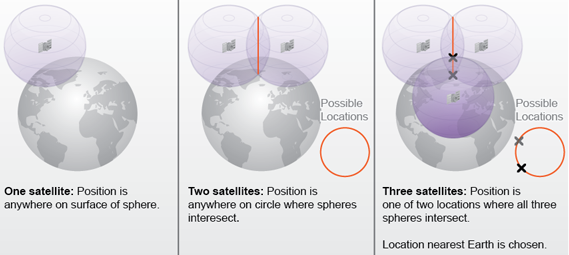
\includegraphics[width=0.8\textwidth]{localization-methods/gnss}
	\caption[Trilateration technique in a global localization system]{Trilateration technique in a global localization system\protect\footnotemark}
	\label{fig:localization-methods_gnss}
\end{figure}
\footnotetext{\url{https://www.e-education.psu.edu/geog160/node/1923}}
%}


\subsubsection{\glsentryfirst{dgps}}

The accuracy of the \gls{gps} position can be increased with the help of local broadcast stations. These stations are fixed and provide information about the corrections that can be made to the satellite signals in order to improve the localization precision.

These corrections are useful to mitigate some of the ambient interference that the satellite signals face. These interferences can range from simple signal reflection in the environment landscape to the more complex interactions with the atmosphere, which can change the speed and path of the radio signals.

The computation of the corrections \cite{Kim2007} is based on the fact that these stations are fixed, and as such, they can compare the location given by the satellite signals with their known location. With this position differential, the appropriate corrections can be calculated and broadcasted to the \gls{gps} receivers.


\subsubsection{\glsentryfirst{agps}}

\gls{agps} systems are a common method used to speed up the \gls{ttff} of a \gls{gps} receiver. They usually rely on the cellphone network to provide location estimation and signal corrections \cite{R.1948}. This information can greatly reduce the \gls{ttff} when there are few satellites visible or their signal is very weak and only temporary available.


\subsubsection{Signal strength geolocation methods}

Signal strength geolocation \cite{Kobayashi2002}, also known as fingerprinting localization \cite{Bshara2010}, is an approximate method that can be used to calculate relative positions.

It relies on the analysis of the signal attenuation from a given access point (like a Wi-Fi router or cellphone tower), to estimate distances. With enough access points (usually 4), an approximate position can be computed.

This type of distance estimation can be useful for indoor navigation, but requires a propagation model of the signal and the environment. If these models aren't accurate, then the localization precision of these methods will be very low.

Although this method is less accurate than the more recent global localization systems (such as \gls{gps}), it can be used without human made infrastructures, and as such, is a viable solution in case of temporary disruption of the \gls{gps} signal.


\subsection{Celestial navigation}

Celestial navigation \cite{Yang2011} relies on the observation of stars, planets or other reference objects, to calculate the latitude and longitude.

The calculation of the position on the surface of the Earth using celestial navigation is similar to trilateration, but in this case, angles are used instead of distances. These angles (delta), are measured between the Earth horizon and the center of the celestial object.

Having the delta, and knowing the relative position of the Earth to the reference object, along with the Greenwich hour time, it is possible to calculate a circle of position (as shown in \cref{fig:localization-methods_celestial-navigation}).

Having at least 3 circles of position, the latitude and longitude can be computed.

Although this method is less accurate than the more recent global localization systems (such as \gls{gps}), it can be used without human made infrastructures, and as such, is a viable solution in case of temporary disruption of the \gls{gps} signal.

%\afterpage{
\begin{figure}[H]
	\centering
	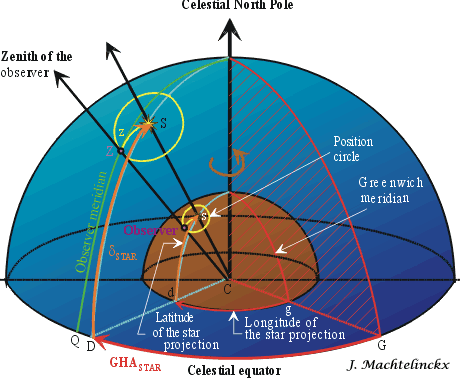
\includegraphics[width=0.45\textwidth]{localization-methods/celestial-navigation}
	\caption[Circle of position in celestial navigation]{Circle of position in celestial navigation\protect\footnotemark}
	\label{fig:localization-methods_celestial-navigation}
\end{figure}
\footnotetext{\url{http://onboardintelligence.com/CelestialNav/Celnav2.aspx}}
%}


\subsection{Landmark methods}

Landmark methods \cite{Lee2006} can be used to perform relative localization, and are very useful to reduce the required information for navigation.

In these methods a database of markers / environment geometry is stored along with its location, and when the robot recognizes one of these markers, it corrects its proprioceptive methods measures.

It is a simplification of the method that will be presented in the next section, and it is useful for environments that have unique geometry in key positions of the navigation map.


\subsection{Point cloud methods}\label{subsec:localization-methods_point-cloud-methods}

Point cloud localization methods can be used to perform relative localization by finding the best point cloud match between the environment and the know map (\cref{fig:localization-methods_icp} shows its application to small objects). These methods require a 2D or 3D representation of the environment and tend to be used in conjunction with proprioceptive methods (to have an estimation of movement), and also with probabilistic methods (when the point cloud acquisition location is not known).

One of the most used algorithms for 3D point cloud matching is the \gls{icp} \cite{Besl1992,Jez2008,Zhang1992,Bouaziz2013,Chetverikov2002,Djehaich2013,Zhou2011}. It is an iterative algorithm that finds the translation and rotation transformation that minimizes the distances of the corresponding points on both clouds. It finishes when the matching error is below a given value, the matrix transformation between iterations has a translation / rotation below the specified thresholds or when the maximum allowed iterations is reached.

There are several variants that optimize different parts of the algorithm \cite{Rusinkiewicz2001}.

The main steps for each iteration of the \gls{icp} algorithm are presented below.

\begin{enumerate}
	\item  Selection of points in one or both point clouds (source and reference clouds)
	\item  Matching / pairing source points to reference points
	\item  Weighting the corresponding pairs
	\item  Rejecting low quality matches (outliers)
	\item  Assigning an error metric based on the point pairs
	\begin{enumerate}
		\item  Usually mean square error based on points distance
	\end{enumerate}
\end{enumerate}


%\afterpage{
\begin{figure}[H]
	\centering
	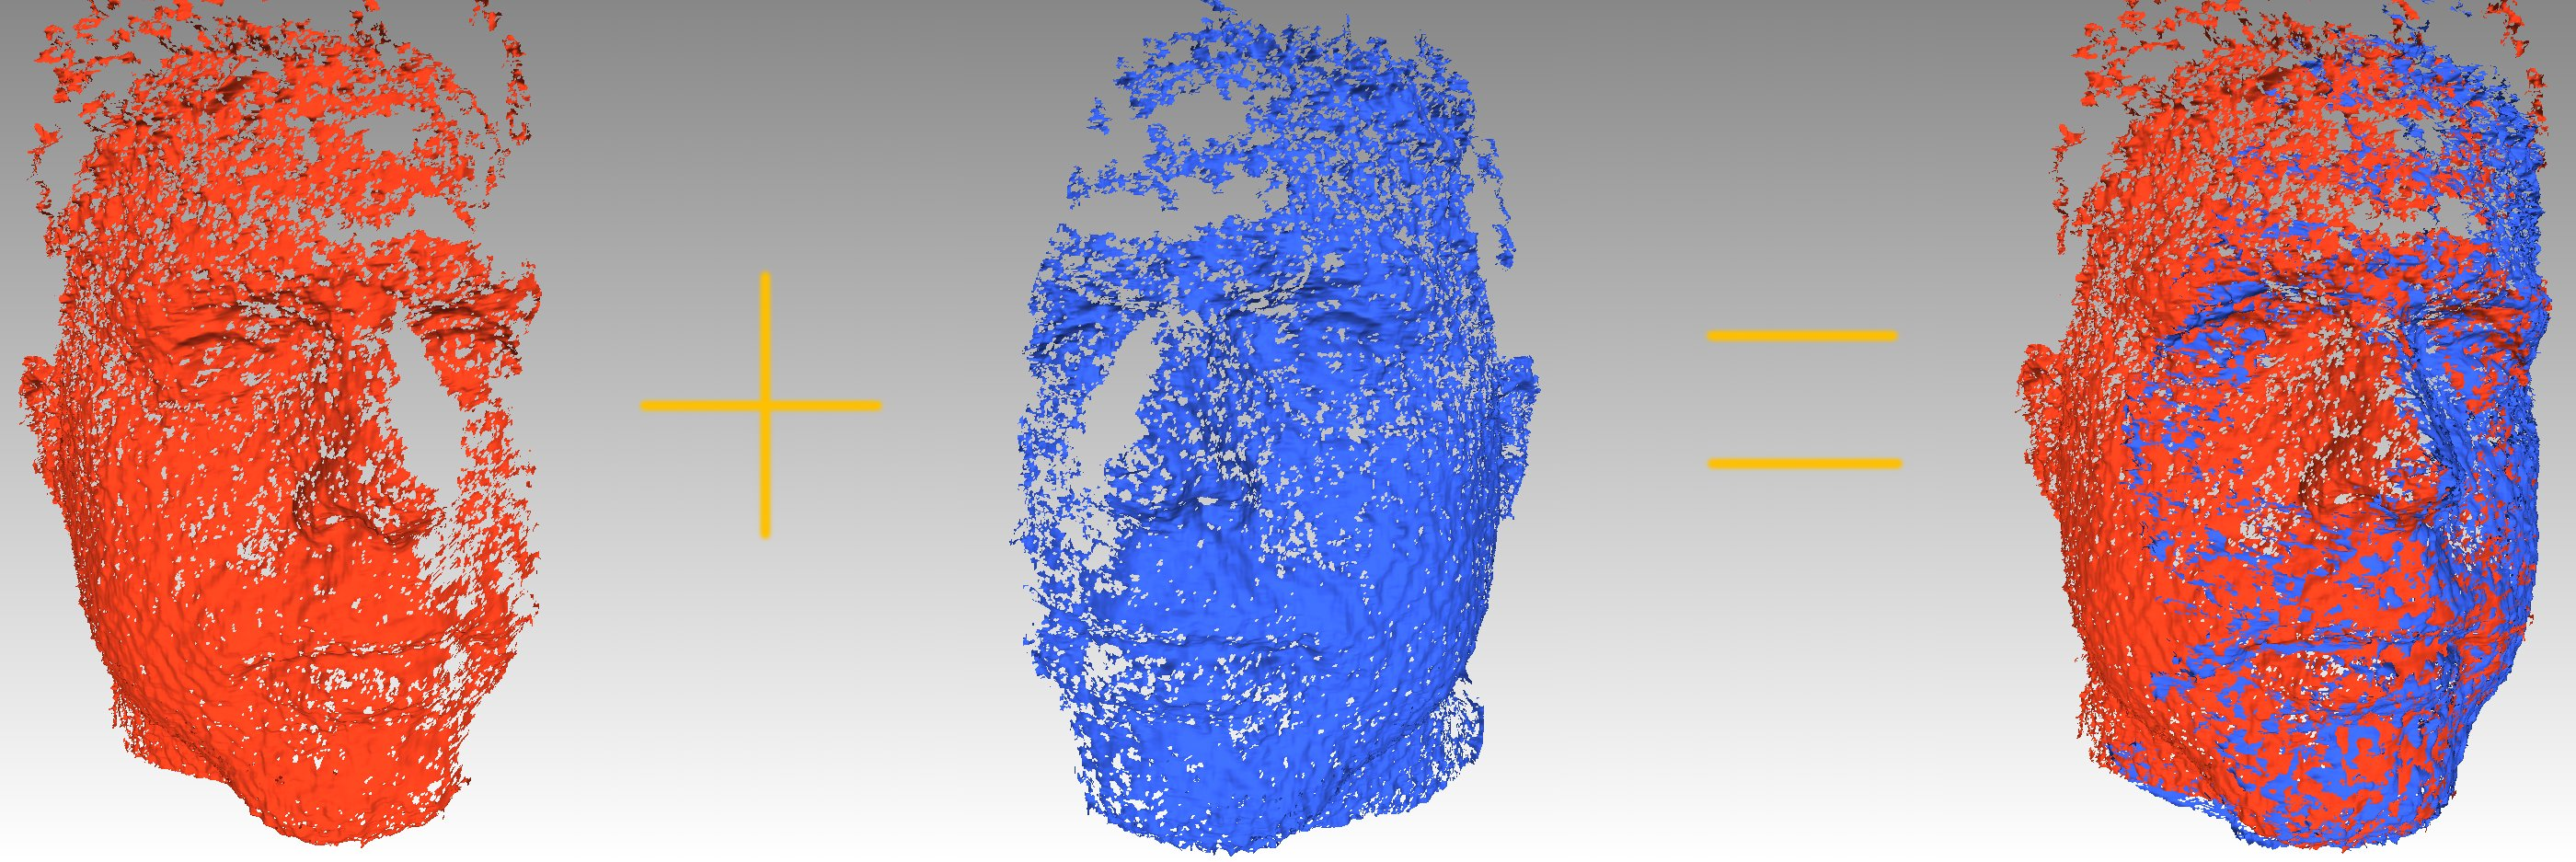
\includegraphics[width=0.75\textwidth]{localization-methods/icp}
	\caption[\glsentrytext{icp} point cloud matching]{\glsentrytext{icp} point cloud matching\protect\footnotemark}
	\label{fig:localization-methods_icp}
\end{figure}
\footnotetext{\url{http://dynface4d.isr.uc.pt/database.php}}
%}


\subsection{Probabilistic methods}

Probabilistic methods aim to reduce the impact of sensor accumulated errors or even temporary malfunctions by using Bayesian estimations and Markov processes.


\subsubsection{\glsentryfirst{mcl}}

\gls{mcl} (also known as particle filter), is a global localization algorithm that estimates the position and orientation of a robot by analyzing and adjusting the distribution and weights of state particles on a given environment \cite{Bshara2010,Arulampalam2002,Blanco2010,Chen2003b,Fox1999,Saito2009}.

It starts by randomly distributing the state particles on the map, and over time it changes their position and weight according to new sensor readings. The probable location of the robot will be in the area of the map that has the largest cluster of state particles. The figures below show the evolution of the state particles distribution during the robot movement in the environment, and illustrates how the new sensor readings changed the particles clusters\footnote{\url{http://www.cs.washington.edu/robotics/mcl/}}.

\begin{figure}[H]
	\centering
	\begin{minipage}[h]{.49\textwidth}
		\centering
		\animategraphics[width=0.9\textwidth,loop,autoplay,controls]{4}{localization-methods/mcl/frame-}{0}{39}
		\caption{\glsentrytext{mcl} animation}
		\label{fig:localization-methods_mcl1}
	\end{minipage}\hfill
	\begin{minipage}[h]{.49\textwidth}
		\centering
		\includegraphics*[width=0.99\textwidth]{localization-methods/mcl-2}
		\caption{\glsentrytext{mcl} redistribution of particles}
		\label{fig:localization-methods_mcl2}
	\end{minipage}
\end{figure}

\begin{figure}[H]
	\centering
	\begin{minipage}[h]{.49\textwidth}
		\centering
		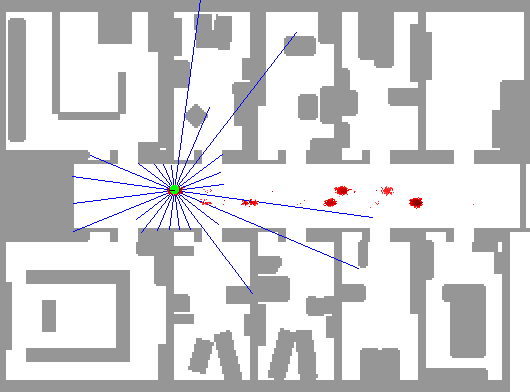
\includegraphics[width=0.99\textwidth]{localization-methods/mcl-3}
		\caption{\glsentrytext{mcl} position refinement}
		\label{fig:localization-methods_mcl3}
	\end{minipage}\hfill
	\begin{minipage}[h]{.49\textwidth}
		\centering
		\includegraphics*[width=0.99\textwidth]{localization-methods/mcl-4}
		\caption{\glsentrytext{mcl} position estimation}
		\label{fig:localization-methods_mcl4}
	\end{minipage}
\end{figure}


\subsubsection{Kalman filters}

Kalman filters \cite{Kalman1960} are probabilistic algorithms that estimate a given system state even when it is affected by noise or other errors. They perform linear quadratic estimations to achieve optimal results and can be efficiently implemented to be used in real time systems. They are recursive algorithms based on Marcov processes, and as a result, they only need to know the current system state in order to perform measurement corrections.

The \gls{ekf} \cite{Einicke1999,Ribeiro2004,Ivanjko2010,Liu2011} is a variant of the Kalman filter, designed to handle non-linear systems by performing linear approximations to the state variables. These approximations may lead to divergence in the estimations, and as such, the \gls{ekf} can't guarantee optimal results.

The \gls{ukf} \cite{Julier1997,Wan2002} is another variant of the Kalman filter that was designed for highly non-linear systems. It usually achieves better results than \gls{ekf} due to its unscented transform.

For the particular case of localization, these algorithms start with an initial estimation of the system state, and for each new position (computed from the sensors data), they predict the estimated robot location (according to the Bayes estimation model and the Gaussian distribution of errors), and then update their internal model of the system (mean and covariance) to incorporate the system evolution.

In \cref{fig:localization-methods_ukf} can be seen that the \gls{ukf} estimated position (red) is closer to the real position (blue) than the raw sensor measurements (green).

%\afterpage{
\begin{figure}[H]
	\centering
	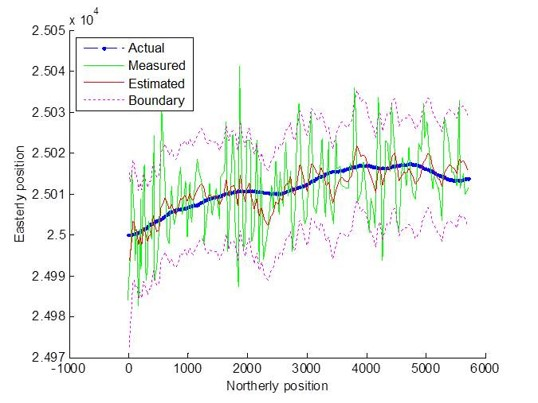
\includegraphics[width=0.9\textwidth]{localization-methods/ukf}
	\caption[Unscented Kalman Filter]{Unscented Kalman Filter\protect\footnotemark}
	\label{fig:localization-methods_ukf}
\end{figure}
\footnotetext{\url{http://www.lzcheng.com/courseworks/kalmanfilter}}
%}


\subsubsection{Perfect Match}

The Perfect Match \cite{Lauer2006a,Pinto1963} is an efficient self-localization algorithm that is largely used in the Robocup Robotic Soccer Mid Size League. Its main goal is to minimize the localization error by carefully analyzing the know map and selecting the most probable current position using a gradient descent approach. To improve tracking accuracy, the algorithm also uses a stochastic weighted approach.

With the proper configuration, it can achieve a localization accuracy similar to the particle filter, while using about ten times less computations.

An example of the position estimation can be seen in the figures below. \Cref{fig:localization-methods_pm-1} shows the probable locations when the robot detects a line on the floor, and \cref{fig:localization-methods_pm-2} illustrates their associated errors (brighter areas indicate smaller error). By using a gradient descent, the most probable location was selected (black circle).

\begin{figure}[H]
	\centering
	\begin{minipage}[h]{.495\textwidth}
		\centering
		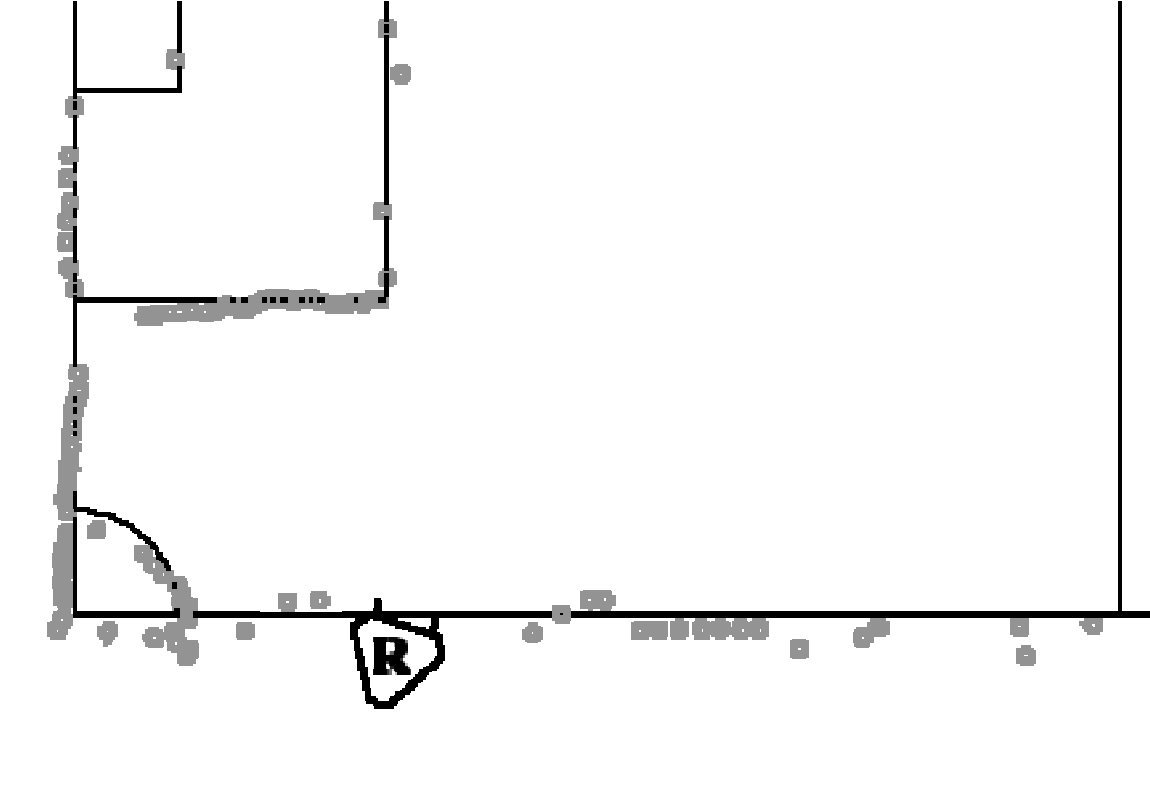
\includegraphics[width=\textwidth]{localization-methods/pm-1}
		\caption{Position estimate}
		\label{fig:localization-methods_pm-1}
	\end{minipage}\hfill
	\begin{minipage}[h]{.495\textwidth}
		\centering
		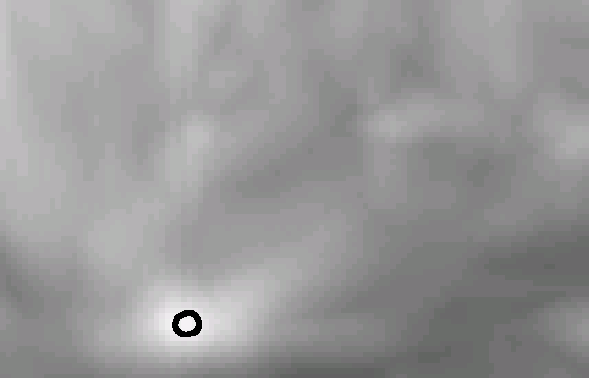
\includegraphics[width=\textwidth]{localization-methods/pm-2}
		\caption{Position associated error}
		\label{fig:localization-methods_pm-2}
	\end{minipage}
\end{figure}


\subsection{\glsentryfirst{slam}}

\gls{slam} \cite{Thrun2002} is a very effective approach to either explore unknown environments or update a known map. It relies on both proprioceptive and exteroceptive methods to perform localization and mapping. It is also very useful to make the robot navigation more robust in dynamic environments, in which the topology of the world may change considerably over time.

There are numerous approaches to perform  \gls{slam} \cite{Tuna2012}. Some optimized for exploration and others for map improvement. For the exploration tasks, proprioceptive methods play a critical role, and are usually paired with probabilistic methods, such as Kalman filters, in order to reliably map the environment. For map correction and improvement, several probabilistic methods can be employed according to the precision required. For high accuracy 3D mapping, the \gls{icp} algorithm can be used to build accurate point clouds of the environment.



\section{Summary}

This chapter introduced several localization systems that can be used in different types of environments and with different degrees of accuracy. It started with the simple proprioceptive methods and then moved on to the more robust exteroceptive approaches.

Some techniques can be combined to improve the pose estimate or to make the localization more efficient to a particular type of environment.

For outside tasks, a \gls{gnss} approach can give accurate localization estimations with very little computation cost. On the other hand, indoor localization requires more advanced techniques in order to infer the current position based on the analysis of the robot surroundings. These techniques usually start with an estimation of the robot movement and then refine it with probabilistic or geometric methods.

\Cref{tab:localization-methods_overview-self-localization-approaches} presents an overview of the mentioned localization techniques.


\begin{sidewaystable}
	\caption{Overview of self-localization approaches}
	\tabulinesep = 0.9ex
	\centering
	\begin{tabu} { X[1.4,m,c] | X[m,c] X[m,c] X[m,c] X[m,c] X[6,m,c] }
		\rowfont{\bfseries\itshape} Method & Ideal environment & Accuracy & Operational cost & Computational cost & Notes \\
		\hline
		Odometry			& Any		& Low		& Low		& Low		& Position estimation is affected by cumulative errors \\
		Dead reckoning		& Any		& Low		& Low		& Low		& Pose estimation is affected by cumulative errors \\
		\gls{gnss}			& Outside	& Medium	& Low		& Low		& Requires a clear line of sight to at least 3 satellites \\
		Signal strength		& Any		& Low		& Low		& Low		& Requires an accurate model for the signal attenuation \\
		Celestial			& Outside	& Low		& Low		& Low		& Requires a clear view of the celestial objects and a nautical almanac \\
		Landmark			& Any		& Medium	& Low		& Medium	& Requires a database of landmarks \\
		\gls{icp}			& Indoors	& High		& Medium	& High		& Requires a detailed 3D representation of the environment \\
		\gls{mcl}			& Indoors	& Medium	& Medium	& Medium	& Inefficient for large areas \\
		Kalman filters		& Any		& Medium	& Low		& Low		& Useful to improve estimations of other methods \\
		Perfect Match		& Any		& Medium	& Low		& Low		& Not ideal for large or dynamic environments \\
		\gls{slam}			& Indoors	& Medium	& Medium	& High		& Adapts well to dynamic environments \\
	\end{tabu}
	\label{tab:localization-methods_overview-self-localization-approaches}
\end{sidewaystable}

\chapter{Relevant software / hardware technologies}\label{chap:relevant-sofware-hardware-technologies}



\section*{}

Robot self-localization in complex environments is a multidisciplinary problem that requires advanced computer software systems. In order to speed up the implementation and deployment of the localization system, several frameworks and libraries were used. Among the most important were \gls{ros} for the system architecture, \gls{pcl} for the point cloud processing and Gazebo for simulation and testing.



\section{\glsentrytext{ros}}

\begin{wrapfigure}{r}{0.25\textwidth}
	\centering
	\includegraphics*[width=0.24\textwidth]{relevant-sofware-hardware-technologies/ros-logo}
	\caption{\glsentrytext{ros} logo}
	\label{fig:relevant-sofware-hardware-technologies_ros-logo}
\end{wrapfigure}

\gls{ros}\footnote{\url{http://www.ros.org/}} \cite{Quigley2009} is a software framework designed to ease the development of robot systems. It provides seamless integration between hardware drivers and software modules, allowing a fast transition between simulation and deployment.

It's an open source project that offers a distributed computing framework with several core libraries and development tools that aims to speedup software prototyping, testing and deployment.


\subsection{Architecture}

The \gls{ros} architecture was designed from the beginning to be a distributed peer-to-peer software framework that could be deployed in several operating systems and implemented in a range of different programming languages. However, given that most of the \gls{ros} community prefers open source software, the Ubuntu\footnote{\url{http://www.ubuntu.com/}}] operating system is the main developing and testing environment, and as such, the recommended choice for \gls{ros} developers. Moreover, considering that robotics research requires software with both performance and maintainability at its core, the C++\footnote{\url{http://www.cplusplus.com/}} programming language is used in most of the available packages, along with Python\footnote{\url{https://www.python.org/}} and Java\footnote{\url{https://www.java.com}}.

Being a distributed computing framework, \gls{ros} relies in network connections and exchange of messages to perform the intended tasks. As such, its architecture was developed to follow a publish / subscribe pattern (\gls{ros} topics\footnote{\url{http://wiki.ros.org/Topics}}) and request and reply communication paradigm (\gls{ros} services\footnote{\url{http://wiki.ros.org/Services}} and actions\footnote{\url{http://wiki.ros.org/actionlib}}). This allows \gls{ros} nodes\footnote{\url{http://wiki.ros.org/Nodes}} (operating system processes) to be deployed in different computing platforms with ease and simplifies testing and exchange of software modules.

The next sections provide a more detailed description of the main \gls{ros} architecture concepts.


\subsubsection{Nodes}

\gls{ros} nodes are operating system processes that are part of the peer-to-peer communication graph. They are the fundamental building blocks of any \gls{ros} system and can be spread among several computing platforms.

In order to manage the communications between nodes, the \gls{ros} framework provides a master node (roscore\footnote{\url{http://wiki.ros.org/roscore}}) that uses \gls{xmlrpc} to maintain a communication graph of the system. This allows nodes to be started without knowing the location (\gls{ip} address and port) of the other nodes in the network and greatly simplifies their integration and exchange. Also, by using \gls{ros} launch files\footnote{\url{http://wiki.ros.org/roslaunch}} (\gls{xml} configuration files), the specification of a system communication data flow and configuration can be easily altered.

Besides handling communications, the master node also manages system configurations through the parameter server. This allows nodes to share and change the system configuration at runtime. However, given that the parameter server is usually queried only when a node starts up, the dynamic reconfigure\footnote{\url{http://wiki.ros.org/dynamic_reconfigure}} \gls{api} can be used instead, if it is necessary to change the configuration of a node when it is already running. This is achieved by providing a callback that is asynchronously called when a configuration change is requested.

The flexibility provided by \gls{ros} in both module integration and exchange can greatly speedup testing and deployment and the possibility of changing the configuration of the system at runtime and restart software modules individually (nodes) is very useful when implementing system supervisors and recovery behaviors.


\subsubsection{Nodelets}

A nodelet\footnote{\url{http://wiki.ros.org/nodelet}} is a special kind of node that aims to reduce the overhead of message exchange. This overhead can be significant when messages are very large, such as point clouds or video. To mitigate this problem, the nodelets exchange pointers to shared memory regions, instead of sending the entire messages between nodes.

To achieve this overhead reduction, some architecture changes are required. The most important being the use of threads instead of processes, and the creation of a superclass that all nodelets must inherit. This leads to the creation of plugin libraries for each nodelet instead of an executable for each node.

Another important change is the introduction of nodelet managers to allow loading and setup of nodelets in different threads inside the same process.

In terms of implementation, the transition from nodes to nodelets requires few code changes and can lead to a significant improvement of the overall system performance.


\subsubsection{Topics}

\gls{ros} topics are named communication buses that follow the publish / subscribe pattern. They provide a simple method for exchanging messages between nodes and allow the decoupling of information production and consumption. This is useful when there are multiple sources of the same information or there are multiple consumers that are interested in processing the same data for different purposes. Moreover, this communication architecture allows to log and replay the exchanged messages, which can be helpful to test different algorithms with the same data.

Currently, topics can use either the \gls{tcp} or \gls{udp} protocols to exchange messages. The \gls{tcp} implementation is used by default and creates a bidirectional channel between each producer and subscriber while guaranteeing the delivery of all messages. The \gls{udp} implementation uses an unreliable and stateless transport approach, in which a subscriber listens to a given broadcast address, and has no guarantee that will receive all messages. As such, \gls{tcp} should be used when all messages must be processed, and \gls{udp} should be considered when the latency and the \gls{tcp} overhead are important issues.


\subsubsection{Services}

\gls{ros} services are named communication buses that follow the request and reply paradigm, in which a node asks for a given service and receives a response according to the data that was sent in the request message and the state of the service node. They are useful to query other nodes state or to request the execution of some behavior / action.


\subsubsection{Actions}

\gls{ros} actions are a special kind of service in which the progress of the request can be queried. They are very useful when the request might take a long time, and gives the caller the necessary information to supervise the execution of the request and if necessary, terminate its execution.


\subsection{Build system}

The latest \gls{ros} build system is named catkin\footnote{\url{http://wiki.ros.org/catkin}}, and is the successor of the original rosbuild\footnote{\url{http://wiki.ros.org/rosbuild}} system. It combines CMake\footnote{\url{http://www.cmake.org/}} macros and Python scripts to allow building multiple dependent projects at the same time. It is a cross-platform build system, organized in packages and meta-packages (group of packages). Each package is a software module that can produce libraries or binaries from source code.

Catkin was designed to deal with complex build configurations, which in the case of \gls{ros} packages involves a considerable amount of build dependencies for each project. As such, catkin provides a build system that can easily find, build and link both \gls{ros} and system dependencies. Moreover, it provides install targets to allow faster code releases and simplifies builds from source for the final users.

Other useful features of the catkin build system are the concepts of workspace and overlays. Catkin uses a workspace with out-of-source builds to keep the source code separate from the build files. This allows the code directory structure to be clean of compiler generated files that are platform dependent. Moreover, it simplifies the concurrent usage of packages (overlay), because catkin gives priority to workspace packages (in relation to system packages). This is particularly useful when it is necessary to modify and test some package that has been released and is installed in the system (without having to uninstall the stable release of that package).

Finally, catkin is a cross-platform build system that can be used to build other projects that use CMake and are not related to \gls{ros}.


\subsection{Development tools}

\gls{ros} provides several development tools that allow introspection and visualization of the system state. They are very useful for testing, debugging and profiling.

The next sections give an overview of the most important \gls{ros} tools that are currently available.


\subsubsection{Graphical User Interface tools}

The \gls{ros} development tools that have graphical user interfaces are aggregated in the rqt framework\footnote{\url{http://wiki.ros.org/rqt}}, and are loaded as plugins at runtime (some can be started as standalone applications).

Currently there is plugins to visualize sensor data (rviz\footnote{\url{http://wiki.ros.org/rviz}}); introspect the contents of topics; log and replay \gls{ros} messages (rosbag\footnote{\url{http://wiki.ros.org/rosbag}}); display node, package and coordinate systems graphs; list and filter debug messages; change configuration of running nodes (dynamic reconfigure); monitor nodes memory and processor usage and much more.


\subsubsection{Command line tools}

The \gls{ros} command line tools\footnote{\url{http://wiki.ros.org/ROS/CommandLineTools}} are split across several executables and can be used for advanced introspection (rosnode, rostopic and rosservice), system configuration (rosparam), package building and management (catkin, rosdep and rosinstall) and also to search \gls{ros} message types documentation (rosmsg and rossrv).

Finally, it is available a diagnostics tool (roswtf), that can detect packages / dependencies issues and configuration problems.



\section{\glsentrytext{pcl}}

\begin{wrapfigure}{r}{0.25\textwidth}
	\centering
	\includegraphics*[width=0.24\textwidth]{relevant-sofware-hardware-technologies/pcl-logo}
	\caption{\glsentrytext{pcl} logo}
	\label{fig:relevant-sofware-hardware-technologies_pcl-logo}
\end{wrapfigure}

The \gls{pcl}\footnote{\url{http://pointclouds.org/}} \cite{Rusu2011} is an open source project that provides algorithms for processing point clouds. These algorithms can be used to filter and register point clouds as well as perform object segmentation, recognition and tracking.

\Cref{fig:relevant-sofware-hardware-technologies_pcl-dependency-graph} gives an overview of the main modules currently available in \gls{pcl}.

%\afterpage{
\begin{figure}[H]
	\centering
	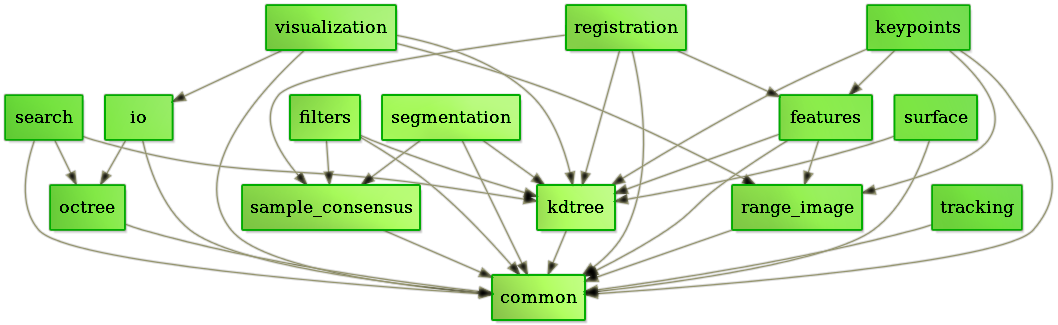
\includegraphics[width=\textwidth]{relevant-sofware-hardware-technologies/pcl-dependency-graph}
	\caption[\glsentrydesc{pcl}]{\glsentrydesc{pcl}\protect\footnotemark}
	\label{fig:relevant-sofware-hardware-technologies_pcl-dependency-graph}
\end{figure}
\footnotetext{\url{http://pointclouds.org/about/}}
%}

\clearpage



\section{Gazebo}

\begin{wrapfigure}{r}{0.25\textwidth}
	\centering
	\includegraphics*[width=0.24\textwidth]{relevant-sofware-hardware-technologies/gazebo-logo}
	\caption{Gazebo logo}
	\label{fig:relevant-sofware-hardware-technologies_gazebo-logo}
\end{wrapfigure}


Gazebo\footnote{\url{http://gazebosim.org/}} is a 3D multi-robot simulator capable of generating hardware sensor data for different kinds of robots while providing a realistic environment with physics simulation and 3D visualization. It is very useful to speedup testing of algorithms with different types of robots and environments.

\Cref{fig:relevant-sofware-hardware-technologies_gazebo-ros-integration} shows how Gazebo can be used instead of a real robot, without requiring any implementation code modification (because it implements the same \gls{ros} interfaces that the hardware drivers use).

%\afterpage{
\begin{figure}[ht]
	\centering
	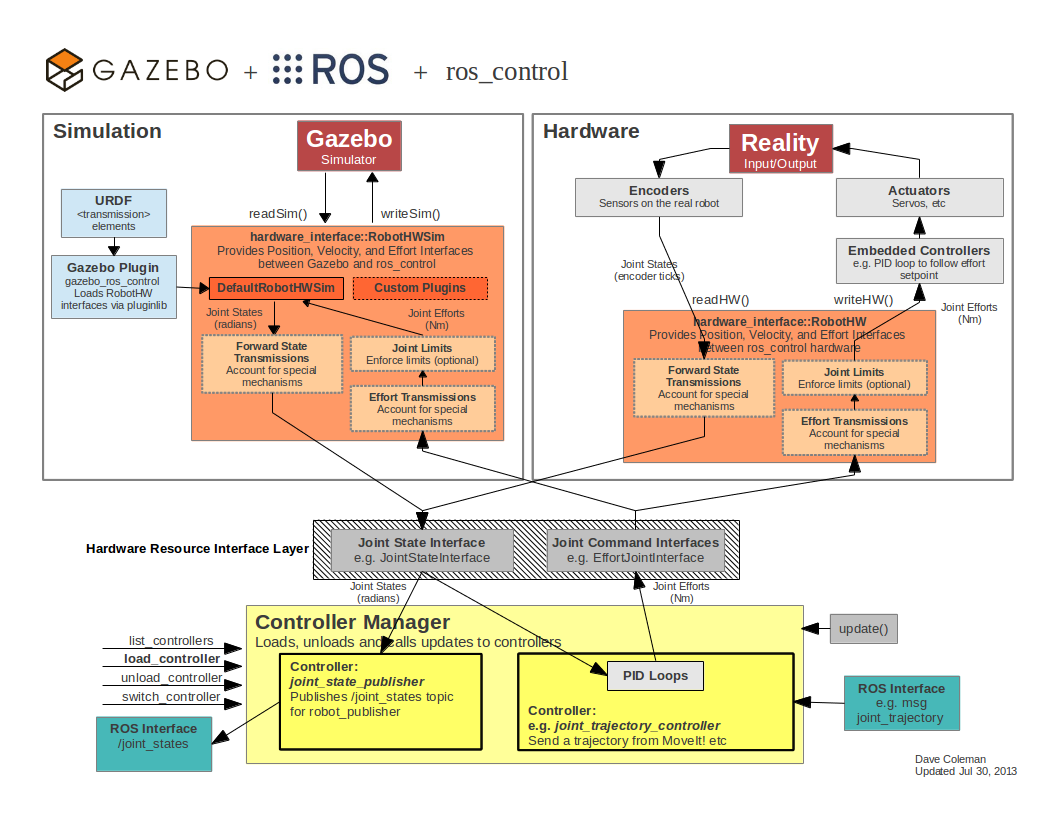
\includegraphics[width=0.8\textwidth]{relevant-sofware-hardware-technologies/gazebo-ros-integration}
	\caption[Integration of \glsentrytext{ros} and Gazebo]{Integration of \glsentrytext{ros} and Gazebo\protect\footnotemark}
	\label{fig:relevant-sofware-hardware-technologies_gazebo-ros-integration}
\end{figure}
\footnotetext{\url{http://gazebosim.org/tutorials?tut=ros_control}}
%}

\clearpage



\section{Point cloud acquisition}\label{sec:relevant-sofware-hardware-technologies_point-cloud-acquisition}

Point clouds can be retrieved with a wide range of sensors with varying levels of precision and assembly time \cite{Sansoni2009}. The next sections provide a brief overview of the three main groups of methods capable of generating point clouds.


\subsection{Structured light methods}

Structured light methods can retrieve 3D geometry from images by projecting a known pattern into the environment and analyzing its deformation (example in \Cref{fig:relevant-sofware-hardware-technologies_structured-light}). They can achieve sample rates of 30 Hz, and besides 3D geometry they can also retrieve color information.

\begin{figure}[H]
	\centering
	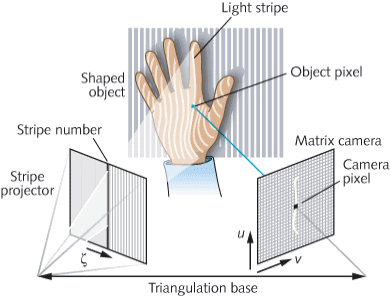
\includegraphics[width=0.5\textwidth]{relevant-sofware-hardware-technologies/structured-light}
	\caption[Structured light system diagram]{Structured light system diagram\protect\footnotemark}
	\label{fig:relevant-sofware-hardware-technologies_structured-light}
\end{figure}
\footnotetext{{\scriptsize \url{http://www.laserfocusworld.com/articles/2011/01/lasers-bring-gesture-recognition-to-the-home.html}}}


The Kinect 2\footnote{\url{http://www.microsoft.com/en-us/kinectforwindows/}} (seen in \cref{fig:relevant-sofware-hardware-technologies_kinect2}) is an example of a structured light system and can achieve measurements with millimeter accuracy for objects close to the sensor. Another similar sensor is Structure IO\footnote{\url{http://structure.io/}} which is intended for mobile devices and can be seen in \cref{fig:relevant-sofware-hardware-technologies_structure-io}.

%\afterpage{
\begin{savenotes}
\begin{figure}[H]
	\centering
	\begin{minipage}[h]{.47\textwidth}
		\centering
		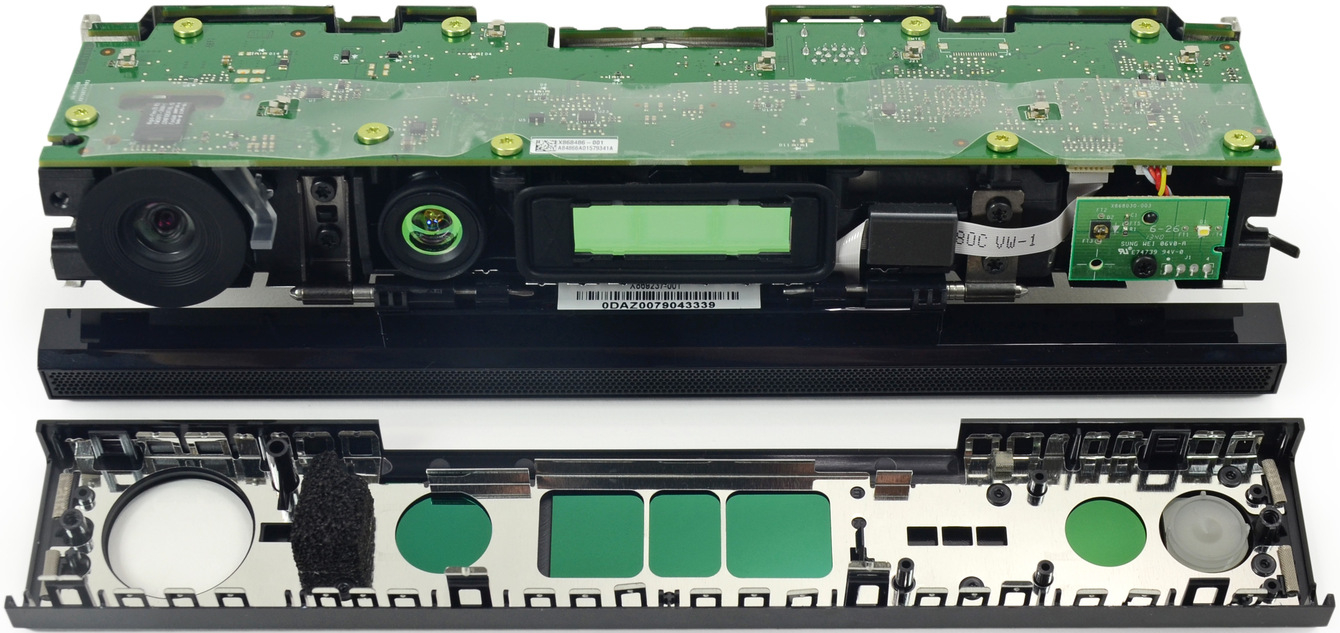
\includegraphics[width=\textwidth]{relevant-sofware-hardware-technologies/kinect2}
		\caption[Kinect 2 sensor]{Kinect 2 sensor\protect\footnotemark}
		\label{fig:relevant-sofware-hardware-technologies_kinect2}
	\end{minipage}\hfill
	\footnotetext{\scriptsize \url{https://www.ifixit.com/Teardown/Xbox+One+Kinect+Teardown/19725}}
	\begin{minipage}[h]{.47\textwidth}
		\centering
		\includegraphics*[width=0.7\textwidth]{relevant-sofware-hardware-technologies/structure-io}
		\caption[Structure IO sensor]{Structure IO sensor\protect\footnotemark}
		\label{fig:relevant-sofware-hardware-technologies_structure-io}
	\end{minipage}
	\footnotetext{\scriptsize \url{http://structure.io/press}}
\end{figure}
\end{savenotes}
%}



\subsection{\glsentrydesc{tof} methods}\label{sec:relevant-sofware-hardware-technologies_tof-methods}

\gls{tof} or \gls{toa} methods can be used to calculate distances based on the amount of time that a given wave takes from the moment it is created to the moment it is received. By assembling a large amount of sensor readings a 3D representation of the environment can be achieved.

Since these systems rely on active interaction with the environment, they can be used without being affected by lighting interferences. Nevertheless, they should take in consideration the conditions in which the waves propagate and also the geometry of the environment, because it can affect the path that the waves take, and as a result, can lead to the decrease of precision in the measurements.


\subsubsection{Light waves}

Light waves generated with lasers can estimate distances with millimeter accuracy at long ranges (system operation overview in \cref{fig:relevant-sofware-hardware-technologies_time-of-flight}) and their sensors usually have a low sample rate (below 20 Hz). Systems like \gls{lidar} (2D sensor example in \cref{fig:relevant-sofware-hardware-technologies_sick-nav-350} and for 3D in \cref{fig:relevant-sofware-hardware-technologies_velodyne-hdl-64e}) take advantage of this fact and can be used to obtain a very detailed 3D point cloud of the environment (like the one showed in \cref{fig:relevant-sofware-hardware-technologies_lidar-scan}). Moreover, some \glspl{lidar} can also capture the environment reflectivity / intensity besides their 3D geometry. On the other hand, \gls{tof} cameras (example in \cref{fig:relevant-sofware-hardware-technologies_mesa-sr4000}) have a very high sample rate (30 Hz or even higher), but have much more measurement error (greater than 1 cm). However, these methods allow the mapping of the environment with low latency, which can be a critical requirement in robots that must react very fast to changes in their surroundings, such as autonomous cars \cite{Moras2010}.

\begin{figure}[H]
	\centering
	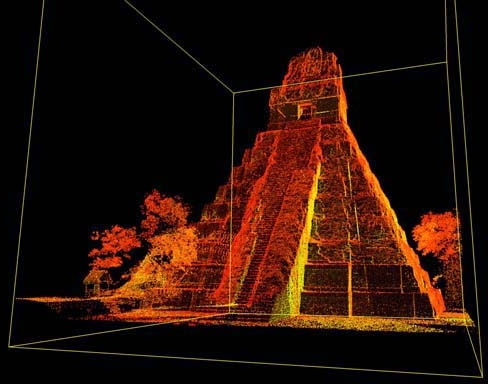
\includegraphics[width=0.6\textwidth]{relevant-sofware-hardware-technologies/lidar-scan}
	\caption[\glsentrytext{lidar} scan]{\glsentrytext{lidar} scan\protect\footnotemark}
	\label{fig:relevant-sofware-hardware-technologies_lidar-scan}
\end{figure}
\footnotetext{\url{http://blogs.scientificamerican.com/cocktail-party-physics/2012/03/12/l-is-for-lidar/}}


%\afterpage{
\begin{savenotes}
\begin{figure}[H]
	\centering
	\begin{minipage}[h]{.47\textwidth}
		\centering
		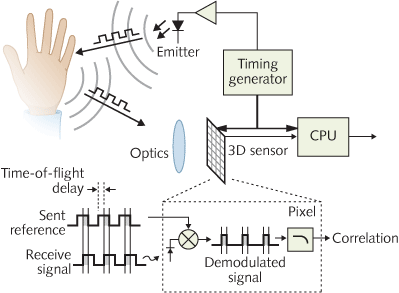
\includegraphics[width=0.8\textwidth]{relevant-sofware-hardware-technologies/time-of-flight}
		\caption[\glsentrydesc{tof} system]{\glsentrydesc{tof} system\protect\footnotemark}
		\label{fig:relevant-sofware-hardware-technologies_time-of-flight}
	\end{minipage}\hfill
\footnotetext{\url{http://www.laserfocusworld.com/articles/2011/01/lasers-bring-gesture-recognition-to-the-home.html}}
	\begin{minipage}[h]{.47\textwidth}
		\centering
		\includegraphics*[width=0.53\textwidth]{relevant-sofware-hardware-technologies/mesa-sr4000}
		\caption[Mesa SR4000]{Mesa SR4000\protect\footnotemark}
		\label{fig:relevant-sofware-hardware-technologies_mesa-sr4000}
	\end{minipage}
	\footnotetext{\scriptsize \url{http://www.mesa-imaging.ch/products/product-overview/}}
\end{figure}
\end{savenotes}
%}


%\afterpage{
\begin{savenotes}
\begin{figure}[H]
	\centering
	\begin{minipage}[h]{.47\textwidth}
		\centering
		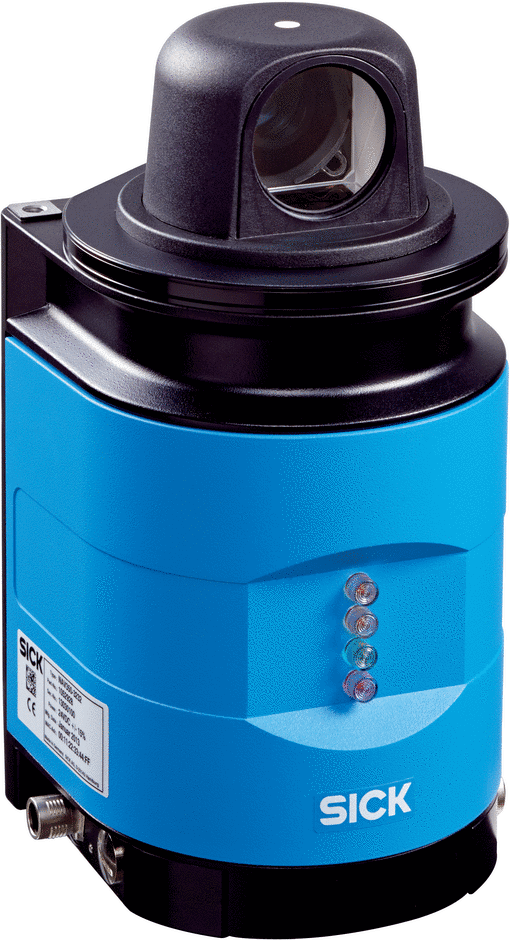
\includegraphics[width=0.4\textwidth]{relevant-sofware-hardware-technologies/sick-nav-350}
		\caption[2D SICK NAV 350]{2D SICK NAV 350\protect\footnotemark}
		\label{fig:relevant-sofware-hardware-technologies_sick-nav-350}
	\end{minipage}\hfill
\footnotetext{\url{https://www.sick.com/de/en/detection-and-ranging-solutions/2d-laser-scanners/nav/nav350-3232/p/p256041}}
	\begin{minipage}[h]{.47\textwidth}
		\centering
		\includegraphics*[width=0.67\textwidth]{relevant-sofware-hardware-technologies/velodyne-hdl-64e}
		\caption[3D Velodyne HDL-64E]{3D Velodyne HDL-64E\protect\footnotemark}
		\label{fig:relevant-sofware-hardware-technologies_velodyne-hdl-64e}
	\end{minipage}
	\footnotetext{\scriptsize \url{http://www.velodynelidar.com/lidar/hdlproducts/hdl64e.aspx}}
\end{figure}
\end{savenotes}
%}


\subsubsection{Radio waves}

Similar to \gls{lidar}, radio waves can be used to calculate distances using the \gls{tof} technique. Systems like \gls{radar} provide an effective way to calculate the distance, altitude, direction and speed of objects that can be used as landmarks in navigation.

Like any electromagnetic wave localization method, it must take in consideration ambient interferences and even jamming, in order to validate the obtained measures. Moreover, some types of materials with a given geometric configuration might be invisible to \gls{radar}, and as such, critical localization systems might have to employ some additional techniques to ensure the correct mapping of the robot surroundings.

Since \gls{radar} has a less focused beam than \gls{lidar}, it can have considerable less accuracy, as can be seen in \cref{fig:relevant-sofware-hardware-technologies_radar-scan}. Nevertheless, it can be an effective method to avoid obstacles \cite{Wu2007}.


%\afterpage{
\begin{savenotes}
\begin{figure}[H]
	\centering
	\begin{minipage}[h]{.47\textwidth}
		\centering
		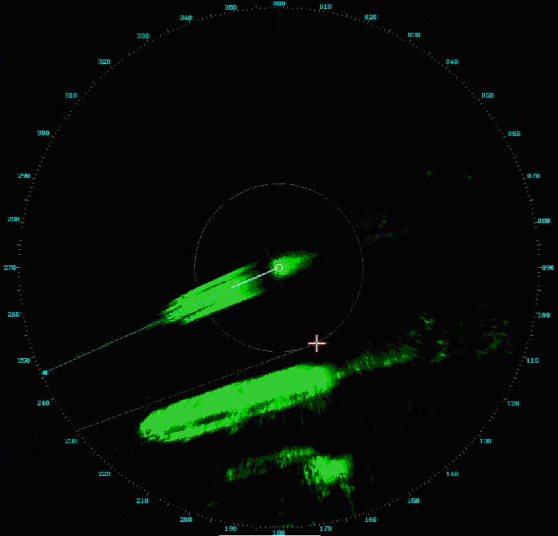
\includegraphics[width=0.9\textwidth]{relevant-sofware-hardware-technologies/radar-scan}
		\caption[\glsentrytext{radar} scan of two ships]{\glsentrytext{radar} scan of two ships\protect\footnotemark}
		\label{fig:relevant-sofware-hardware-technologies_radar-scan}
	\end{minipage}\hfill
	\footnotetext{\scriptsize \url{http://www.sintef.no/Projectweb/STSOps/News/Operational-Aspects-on-Decision-making-in-STS-Lightering}}
	\begin{minipage}[h]{.47\textwidth}
		\centering
		\includegraphics*[width=0.7\textwidth]{relevant-sofware-hardware-technologies/radar-qt50r}
		\caption[QT50R-AFH \glsentrytext{radar}]{QT50R-AFH \glsentrytext{radar}\protect\footnotemark}
		\label{fig:relevant-sofware-hardware-technologies_radar-qt50r}
	\end{minipage}
	\footnotetext{\scriptsize \url{http://www.bannerengineering.com/en-US/products/8/Sensors/658/Radar-Sensors/617/R-GAGE-QT50R-AFH-Adjustable-Field\%2C-High-Sensitivity-Sensor/}}
\end{figure}
\end{savenotes}
%}



\subsubsection{Sound waves}

Another type of 3D sensor that can be used to map under water environments relies in the acoustic analysis of the reflections of sounds in the surrounding objects. Like the previous methods, \gls{sonar} can actively scan the environment to calculate the locations of the objects using a \gls{tof} technique (as can be seen in \cref{fig:relevant-sofware-hardware-technologies_sonar-scan}). Although this method is usually applied to underwater mapping, it can also be used in other sound propagation environments, such as air \cite{Guarato2013}.

%\afterpage{
\begin{savenotes}
\begin{figure}[H]
	\centering
	\begin{minipage}[h]{.47\textwidth}
		\centering
		\includegraphics*[width=0.9\textwidth]{relevant-sofware-hardware-technologies/sonar-scan}
		\caption[\glsentrytext{sonar} scan of two ships]{\glsentrytext{sonar} scan of two ships\protect\footnotemark}
		\label{fig:relevant-sofware-hardware-technologies_sonar-scan}
	\end{minipage}
	\footnotetext{\scriptsize \url{http://stellwagen.noaa.gov/maritime/palmercrary.html}}
	\begin{minipage}[h]{.47\textwidth}
		\centering
		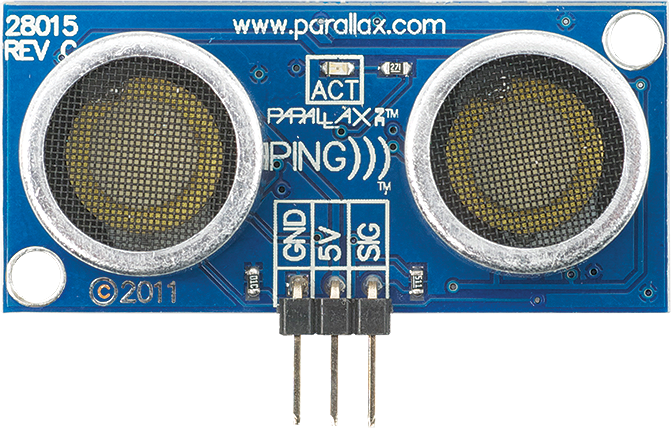
\includegraphics[width=\textwidth]{relevant-sofware-hardware-technologies/sonar-ping}
		\caption[\glsentrytext{sonar} sensor]{\glsentrytext{sonar} sensor\protect\footnotemark}
		\label{fig:relevant-sofware-hardware-technologies_sonar-ping}
	\end{minipage}\hfill
	\footnotetext{\scriptsize \url{http://www.parallax.com/product/28015}}
\end{figure}
\end{savenotes}
%}


\subsection{Stereo vision}

Stereo vision systems (example in \cref{fig:relevant-sofware-hardware-technologies_stereo-cameras}) can generate 3D representations of the environment by comparing the displacement of corresponding points in the two ambient images (\cref{fig:relevant-sofware-hardware-technologies_stereo-vision} gives an overview of such a system). This can be achieved because the relative position of the cameras is known. As such, points farther away will have smaller displacement between images than points closer to the cameras. In the end, a disparity image is obtained, that can then be converted to a point cloud representation of the environment.

Given that the accuracy of the disparity image relies heavily in the correct matching of points between the left and right image, some stereo vision systems employ active observation by projecting a pattern into the environment in order to refine the point matching (example of hardware setup in \cref{fig:relevant-sofware-hardware-technologies_pr2-active-stereo}). This can significantly improve the accuracy if the environment has a lot of smooth surfaces with homogeneous colors.


\begin{figure}[H]
	\centering
	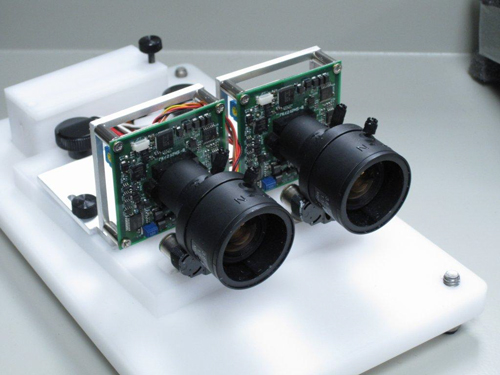
\includegraphics[width=0.55\textwidth]{relevant-sofware-hardware-technologies/stereo-cameras}
	\caption[Stereo vision system]{Stereo vision system \cite{Kaczurba2013}}
	\label{fig:relevant-sofware-hardware-technologies_stereo-cameras}
\end{figure}


\begin{figure}[H]
	\centering
	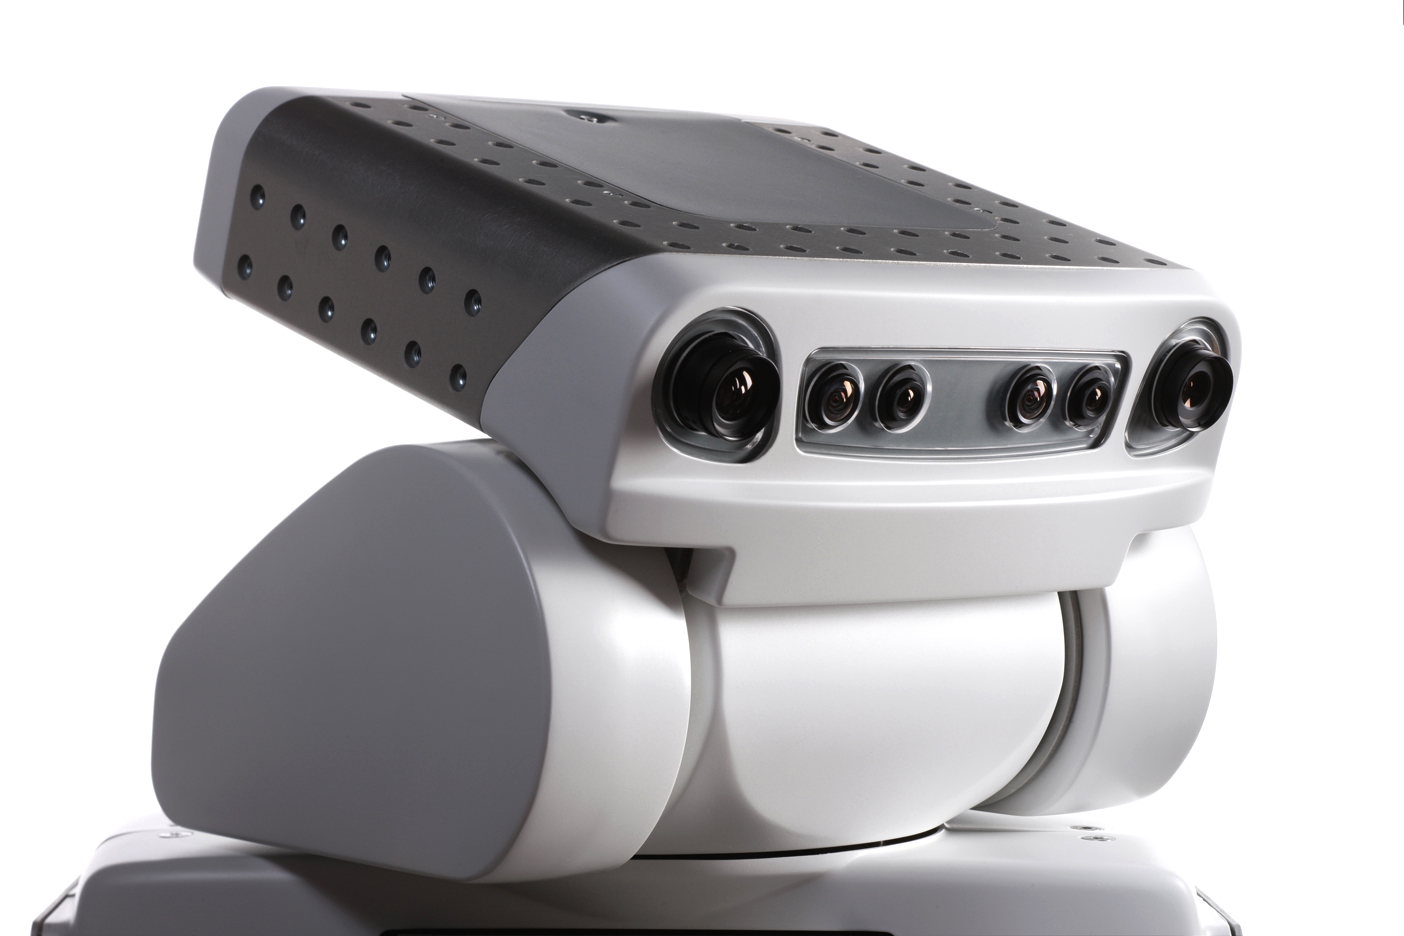
\includegraphics[width=0.55\textwidth]{relevant-sofware-hardware-technologies/pr2-active-stereo}
	\caption[PR2 head capable of active stereo vision]{PR2 head capable of active stereo vision\protect\footnotemark}
	\label{fig:relevant-sofware-hardware-technologies_pr2-active-stereo}
\end{figure}
\footnotetext{\url{https://www.willowgarage.com/pages/pr2/overview}}


\begin{figure}[hb]
	\centering
	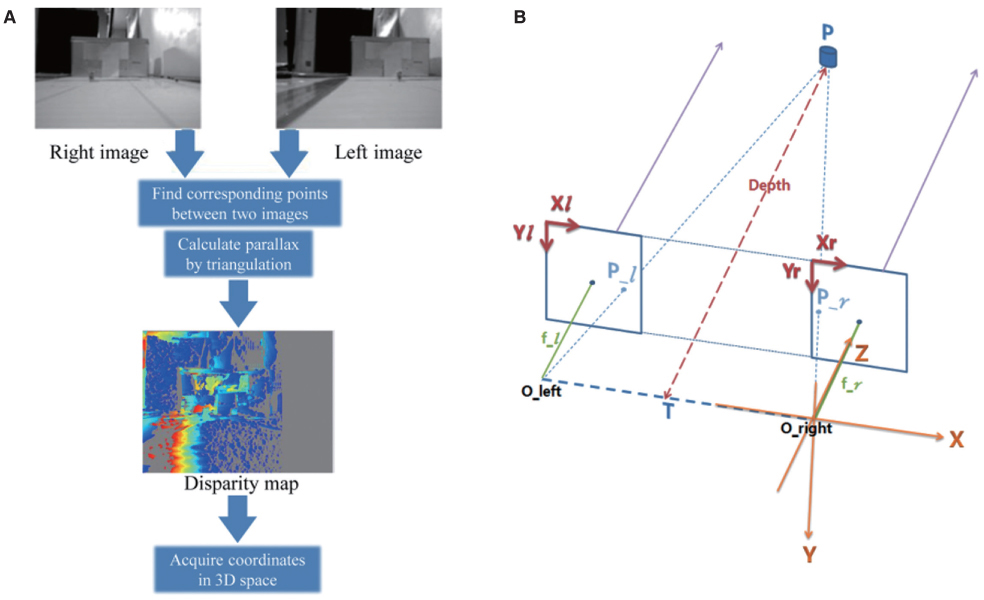
\includegraphics[width=\textwidth]{relevant-sofware-hardware-technologies/stereo-vision}
	\caption[Stereo vision overview]{Stereo vision overview \cite{Yang2014}}
	\label{fig:relevant-sofware-hardware-technologies_stereo-vision}
\end{figure}

\clearpage

\chapter{Localization system} \label{chap:localization-system}



\section*{}

This chapter details the \gls{ros} implementation of the proposed 3/6 \gls{dof} self-localization system\footnote{\url{https://github.com/carlosmccosta/dynamic_robot_localization}}. It starts with an overview of the main processing stages and then details the control flow and algorithms within the localization pipeline.



\section{Overview}

The self-localization system was implemented as a \gls{ros} package and provides 3/6 \gls{dof} localization by publishing \emph{geometry\_msgs::PoseStamped}\footnote{\url{http://docs.ros.org/api/geometry_msgs/html/msg/PoseStamped.html}} and \emph{geometry\_msgs::TransformStamped}\footnote{\url{http://docs.ros.org/api/geometry_msgs/html/msg/TransformStamped.html}} messages along with a detailed analysis of the pose estimation and registered point cloud (split into inliers and outliers). Moreover, it also gives detailed analysis of the computation runtime of each of its modules in order to pinpoint which algorithms are using more computation resources, which is very useful information when configuring or upgrading the system.

The \gls{ros} implementation can receive sensor data through \emph{sensor\_msgs::PointCloud2}\footnote{\url{http://docs.ros.org/api/sensor_msgs/html/msg/PointCloud2.html}} messages and as a result it can directly use data from RGB-D and \gls{tof} cameras. To use \glspl{lidar} it provides an assembler that can produce point clouds by merging measurements from several sensor scans using spherical interpolation. As such, if the \gls{lidar} sensors are mounted on tilting platforms, they can emulate a 3D sensor and retrieve a very detailed view of the environment.

The self-localization system has a modular software architecture and was implemented as several C++ templated shared libraries that can be easily used for other applications besides robot self-localization. As can be seen in \cref{fig:localization-system_localization-system-overview}, it is an extensible and flexible system able to fit the needs of a wide range of mobile platforms. It can be configured as a tracking system, with or without pose recovery and can also have initial pose estimation using feature detection and matching. Moreover, it can dynamically create and update the map if necessary.

It supports two configurable processing pipelines in order to allow fast deployment of robots in large environments. One to process new reference maps and another to localize a mobile robot platform using ambient point clouds. This enables the loading of either processed or unprocessed referenced point clouds and allows a navigation supervisor to dynamically provide the relevant map sections based on the robot position (in order to reduce the computation resources needed).


\begin{figure}[H]
	\centering
	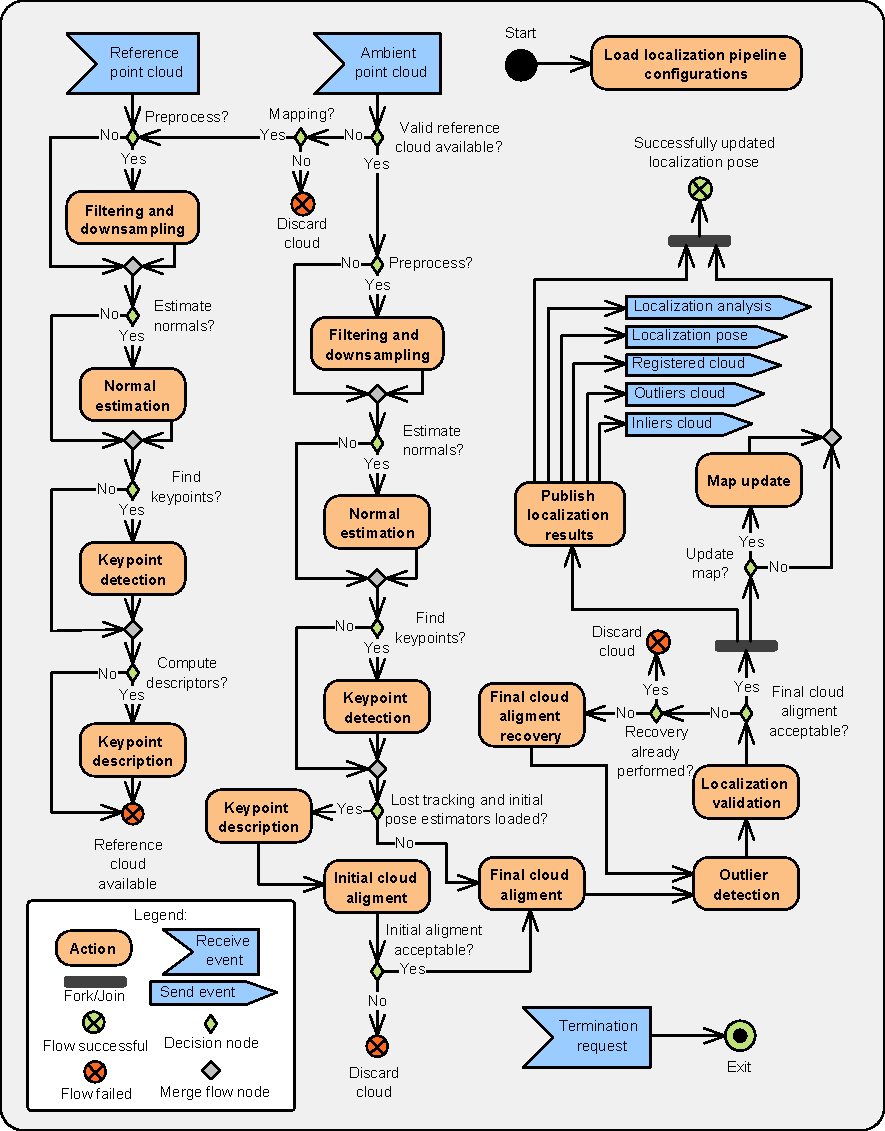
\includegraphics[width=\textwidth]{localization-system/localization-system-overview}
	\caption{Localization system overview}
	\label{fig:localization-system_localization-system-overview}
\end{figure}



\section{Pipeline configuration}

The self-localization system was designed to allow fast reconfiguration\footnote{\url{https://github.com/carlosmccosta/dynamic_robot_localization/blob/hydro-devel/yaml/schema/drl_configs.yaml}} and parameterization through the use of yaml\footnote{\url{http://yaml.org/}} files and the \gls{ros} parameter server\footnote{\url{http://wiki.ros.org/Parameter\%20Server}}. This gives the possibility to quickly tune the localization system to the specific needs of a given mobile platform moving in a particular environment, in order to use the least amount of computational resources possible and without requiring any reprogramming or source code modification. Nevertheless, the system can use a generic configuration if hardware resources are not a concern.

In a typical configuration (following the \emph{Yes} paths of the activity diagram in \cref{fig:localization-system_localization-system-overview}), the first time the localization system is used, it receives a raw reference point cloud that is preprocessed and saved to long term memory along with its associated keypoints and keypoint descriptors. This allows a much faster startup the next time the localization system is initialized. After having a reference point cloud, the localization system will estimate the robot pose periodically by analyzing the ambient point cloud sensor data. This data can be preprocessed with several filters and can be associated with computed surface normals. The robot pose estimation is performed by applying a matrix transformation correction to the current robot pose and is based on the registration of the ambient point cloud with the know map. This registration can use a tracking algorithm configuration tuned for efficiency and a second configuration for tracking recovery purposes. These tracking algorithms require a initial pose estimation, and as such, if one isn't available, a third configuration can be employed to estimate the global position of the robot based on geometric features of the environment. The switch between these configuration is based on the analysis of the registered cloud metrics, such as outlier percentage, inliers root mean square error, inliers angular distribution and the registration corrections performed on the ambient point cloud. After successfully performing the robot pose estimation, the map can be updated by either integrating the full registered point cloud, its inliers or its outliers. Finally, like most \gls{ros} nodes, the localization system will stop its execution when it receives a termination signal request.

The next sections explain in detail the architecture and algorithms used in each of the processing modules present in \cref{fig:localization-system_localization-system-overview}.



\section{Reference map}

The reference point cloud can be loaded from a \gls{cad} file, point cloud file or dynamically arrive trough a \gls{ros} topic as either a 3 \gls{dof} \emph{nav\_msgs::OccupancyGrid}\footnote{\url{http://docs.ros.org/api/nav_msgs/html/msg/OccupancyGrid.html}} or 6 \gls{dof} \emph{sensor\_msgs::PointCloud2}\footnote{\url{http://docs.ros.org/api/sensor_msgs/html/msg/PointCloud2.html}}. This allows a localization supervisor to give only sections of a global map in order to use the least amount of memory and processing power (very large maps have deeper search structures, such as kd-trees, and should be avoided in order to improve the system efficiency).



\section{Point cloud assembly}

The self-localization system can use any sensor that provides point clouds, namely RGB-D / \gls{tof} cameras, \glspl{lidar} and stereo vision systems. Each of these types of sensors have very different operation rates and measurement accuracy. As such, the localization system allows the assembly of several ambient scans using a circular buffer in order to reduce the impact of sensor noise.

For \glspl{lidar}, the system provides a \emph{sensor\_msgs::LaserScan}\footnote{\url{http://docs.ros.org/api/sensor_msgs/html/msg/LaserScan.html}} assembler\footnote{\url{https://github.com/carlosmccosta/laserscan_to_pointcloud}} that converts laser measurements in polar coordinates into Cartesian coordinates and projects the points using spherical interpolation (in order to account for laser scan deformation that occurs when the robot is moving and rotating). It can merge scans from several lasers sensors and it will publish the final point cloud after assembling a given number of scans or periodically after a specified duration. These assembly configurations can be changed at runtime based on the robot velocity (for example, when the robots moves slower, more laser scans are assembled for each published point cloud) or through the use of the \gls{ros} dynamic reconfigure \gls{api}, which allows a navigation supervisor to control the rate at which the localization system operates.



\section{Point cloud search data structures}

Most of the point cloud algorithms use neighbor searches to analyze the surroundings of a given point. As such, efficient data structures are needed to speedup these operations, in order to execute the algorithms efficiently.


\subsection{Voxel grids}

A voxel grid is a three dimensional space partition data structure that splits the Euclidean space into regular voxels (volume pixel). It can be built very fast but is not very efficient for sparse point clouds. \Cref{fig:localization_system_voxel-grid} shows voxel grids with different voxel size.

\begin{figure}[H]
	\centering
	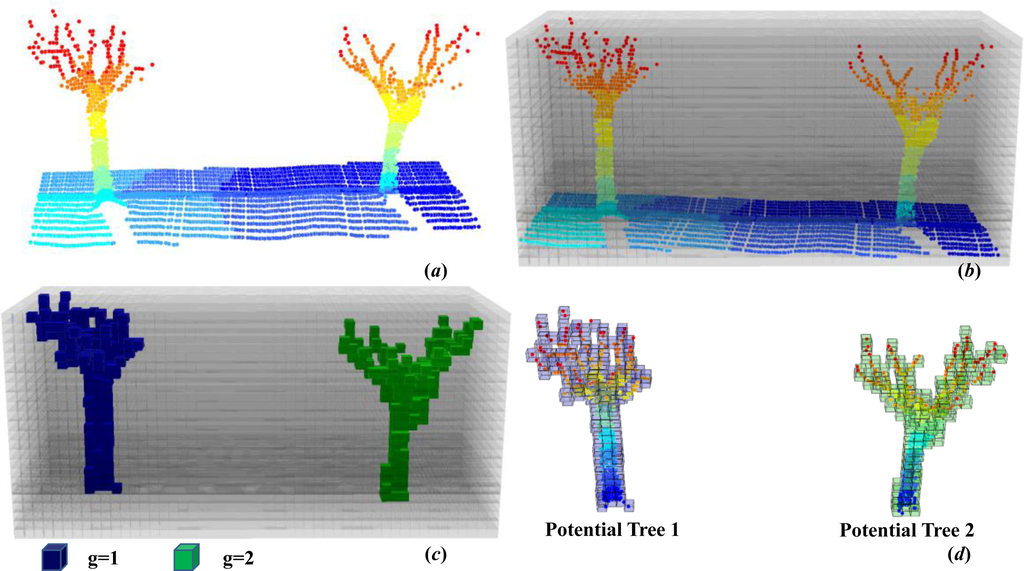
\includegraphics[width=0.7\textwidth]{localization-system/voxel-grid}
	\caption[Voxel grid applied over trees point clouds]{Voxel grid applied over trees point clouds \cite{Wu2013}}
	\label{fig:localization_system_voxel-grid}
\end{figure}



\subsection{Octrees}

An octrees is a hierarchical space partition technique that adapts its tree data structure to the distribution of points in the cloud. It accomplishes this by recursively dividing each voxel in 8 octants until the tree depth is reached or when there is no more points in that region of space. This can be seen in \cref{fig:localization_system_octree} in which areas with no points have large voxels while areas with high point density have much smaller voxels.

%\afterpage{
\begin{figure}[H]
	\centering
	\begin{minipage}[h]{.495\textwidth}
		\centering
		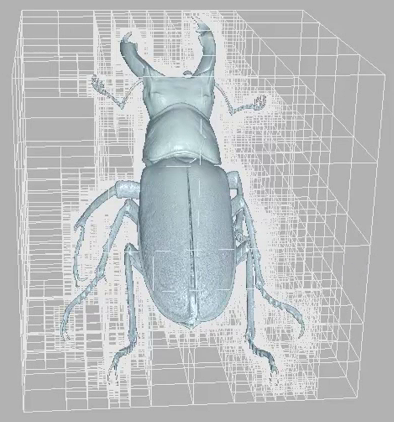
\includegraphics[width=0.55\textwidth]{localization-system/octree-1}
	\end{minipage}\hfill
	\begin{minipage}[h]{.495\textwidth}
		\centering
		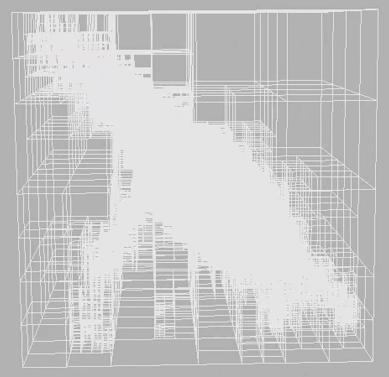
\includegraphics[width=0.6\textwidth]{localization-system/octree-2}
	\end{minipage}
	\caption[Octree of a stag beetle]{Octree of a stag beetle\protect\footnotemark}
	\label{fig:localization_system_octree}
\end{figure}
\footnotetext{\url{http://blog.mpanknin.de/?p=753}}
%}



\subsection{k-d trees}

A k dimensional tree is a space partition technique that can organize points with k dimensions. It is a generic data structure that can be used for 2D and 3D points (examples in \cref{fig:localization_system_2d-tree} and \cref{fig:localization_system_3d-tree}) as well as any other types of data that have an arbitrary number of dimensions (such as point cloud feature descriptors).

The binary k-d tree is built by successively selecting the median point in each axis until all points are inserted in the tree (the selection of the next axis is performed in a circular way, which in the case of three dimensional data, means that after processing the z axis, the x axis would be selected).

%\afterpage{
\begin{savenotes}
\begin{figure}[H]
	\centering
	\begin{minipage}[h]{0.495\textwidth}
		\centering
		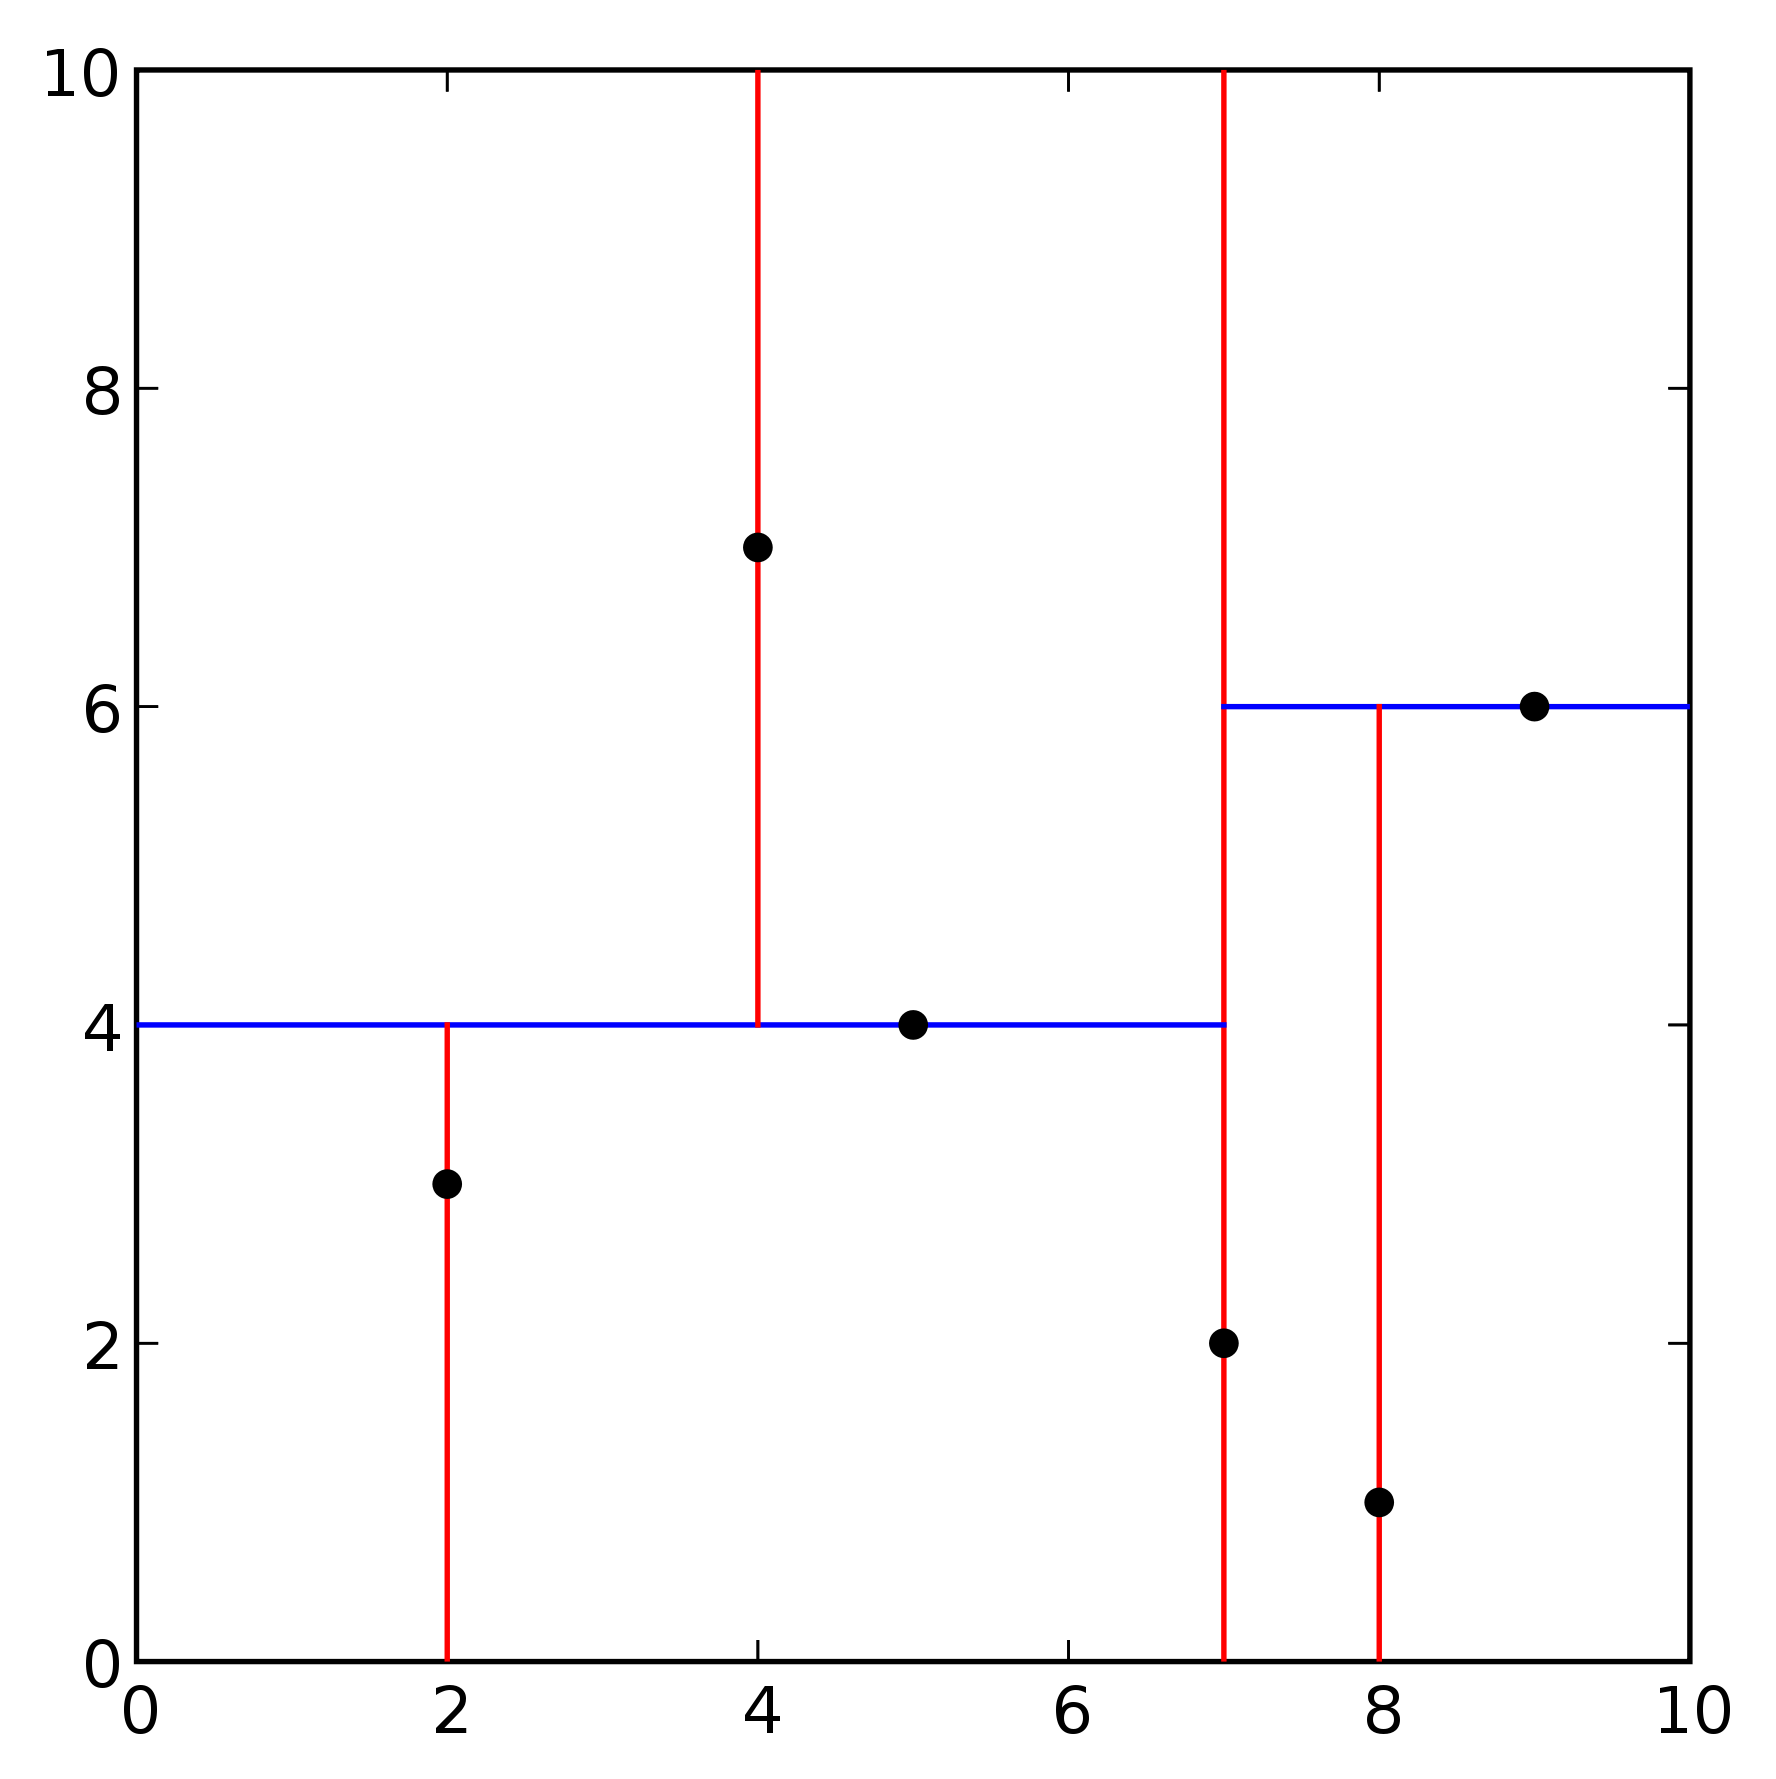
\includegraphics[width=0.55\textwidth]{localization-system/kdtree-2d}
		\caption[2-d tree]{2-d tree\protect\footnotemark}
		\label{fig:localization_system_2d-tree}
	\end{minipage}\hfill
	\footnotetext{\url{http://en.wikipedia.org/wiki/K-d_tree}}
	\begin{minipage}[h]{0.495\textwidth}
		\centering
		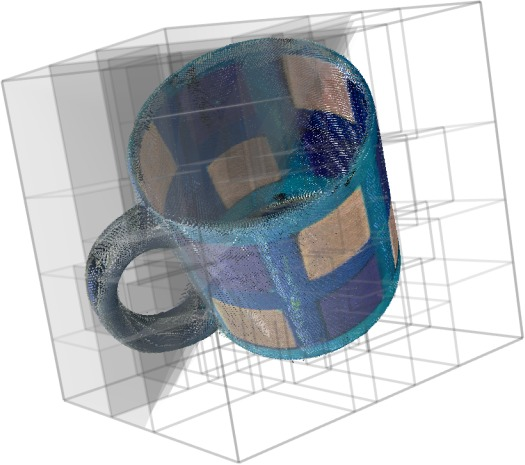
\includegraphics[width=0.6\textwidth]{localization-system/kdtree-3d}
		\caption[3-d tree]{3-d tree\protect\footnotemark}
		\label{fig:localization_system_3d-tree}
	\end{minipage}
	\footnotetext{\url{http://docs.pointclouds.org/trunk/group__kdtree.html}}
\end{figure}
\end{savenotes}
%}



\section{Filtering and down sampling}

The time it takes to perform cloud registration is proportional to the amount of points in the ambient point cloud and in the reference map. As such, adjusting the level of detail of the point clouds by using voxel grids gives some control over the desired localization accuracy and the computational resources that will be required. This stage is also useful to mitigate the measurement errors of the depth sensors, since the centroid of a voxel that contains points from several scans will be closer to the real surface (if the voxels have dimensions slightly larger than the expected measurement errors).

The localization system allows the application of several preprocessing algorithms (algorithm type / configuration and execution order customizable). The next sections detail some of these methods that can be used to filter and downsample point clouds.


\subsection{Point cloud downsampling}

Downsampling methods aim to reduce the number of points while maintaining the surface structure of a given point cloud. They can be used to adjust the level of detail according to the point cloud registration precision required.


\subsubsection{Voxel grid sampling}

A voxel grid is a uniform space partition technique that can be used to cluster points according to their Euclidean coordinates. As can be seen in \cref{fig:localization_system_voxel-grid-downsampling}, it is a very effective method to control the level of detail of a point cloud because it gives the ability to specify the maximum number of points that a region of space should have.

The point cloud downsampling is achieved by replacing each voxel cluster with a single point. The selection of this point can be very fast if the voxel center is used, but computing the centroid of the cluster yields better results because it represents the underlying surface with more accuracy and it attenuates errors in the sensors measurements.


%\afterpage{
\begin{figure}[H]
	\centering
	\begin{minipage}[h]{0.495\textwidth}
		\centering
			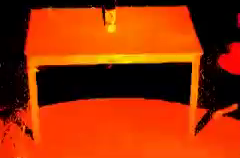
\includegraphics[width=0.97\textwidth]{localization-system/voxel-grid-downsampling-1}
	\end{minipage}\hfill
	\begin{minipage}[h]{.495\textwidth}
		\centering
	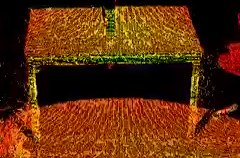
\includegraphics[width=0.97\textwidth]{localization-system/voxel-grid-downsampling-2}
	\end{minipage}
	\caption[Table point cloud before (left) and after (right) voxel grid downsampling]{Table point cloud before (left) and after (right) voxel grid downsampling\protect\footnotemark}
	\label{fig:localization_system_voxel-grid-downsampling}
\end{figure}
\footnotetext{\url{http://pointclouds.org/documentation/tutorials/voxel_grid.php}}
%}



\subsubsection{Random sampling}

Random sampling \cite{Vitter1984} is a fast downsampling method that randomly selects points from the input cloud until the specified number of samples is reached. This has the advantage of using real measures instead of downsampled approximations, but also means it is more sensible to sensor measurements noise. However, for outdoor environments or very complex scenes, using the real measurements can be preferable than using cluster centroids because the voxels may not have the necessary resolution or may have a prohibitive computational cost.


\subsection{Outlier removal}

Some depth sensors can perform measurements with high accuracy, but they have some limitations that can lead to the creation of outliers \cite{Sotoodeh2006}.

One of those limitations can produce shadow points around objects boundaries. This is due to the fact that a portion of the laser beam may hit the object boundary and other part may hit other areas in the object background. And given that most laser range finders use a weighted sum of several beams, this can yield measurements that are not associated with any real object (outliers). \Cref{fig:localization_system_voxel-grid-downsampling} shows a considerable amount of these shadow points close to the front table legs. Another issue is related to the angle in which the depth sensor sees the objects areas. If the incidence angle is very low, then it may be difficult to compute its distance and detect if the beam had ambient reflections. This can significant increase the measurements noise or even lead to the creation of outliers. Other common problem is associated with the material properties of the surfaces. For example, objects with very high or very low reflectance, such as metals or glass, can increase the measurements noise. Moreover depending on the combination of surface geometry, material and incidence angle, some objects may even be undetectable by depth sensors.

Given the negative effect that outliers have in surface normal computation and registration algorithms, they should be removed in a preprocessing stage. There are several approaches to perform outlier detection and removal \cite{YangZhang2010}, ranging from simple distance thresholds to more robust statistical analysis. The next sections present some of then that can be useful in a localization system.


\subsubsection{Distance filter}

Given that depth sensors have a maximum recommended distance for their measurements, it is wise to remove points that are close or beyond this limit. Moreover, it may be useful to remove points that are too close to the sensor, because they may belong to the robot itself and not the environment.

This can be achieved by applying a minimum and maximum threshold to the distances returned by the depth sensor.


\subsubsection{Passthrough filter}

A passthrough filter can select or remove points according to their properties.

For outlier removal, it can be used to select points that are within a given bounding box (useful when we already know what area of the environment we want to analyze) or remove points that don't have the appropriate intensity or color.


\subsubsection{Radius outlier removal filter}

The radius outlier removal filter deletes points that don't have a minimum number of neighbors within a specified radius distance. It can be useful when the point density is known and is very effective in removing isolated points.


\subsubsection{Statistical outlier removal filter}

The statistical outlier removal filter \cite{Rusu2010a} performs a global analysis of the distances between points and discards the ones that don't follow the global distance distribution.

It is a robust filter that adapts itself to the point cloud density and is very effective in removing shadow points. To do so, it computes the mean distance that each point has to a given number of neighbors and builds a global distance distribution (example in \cref{fig:localization_system_statistical-outlier-removal}). Then, assuming that the distribution is Gaussian, it discards the points that have a distance higher than a given threshold (that is a percentage of the standard deviation of the distance distribution).

%\afterpage{
\begin{figure}[H]
	\centering
	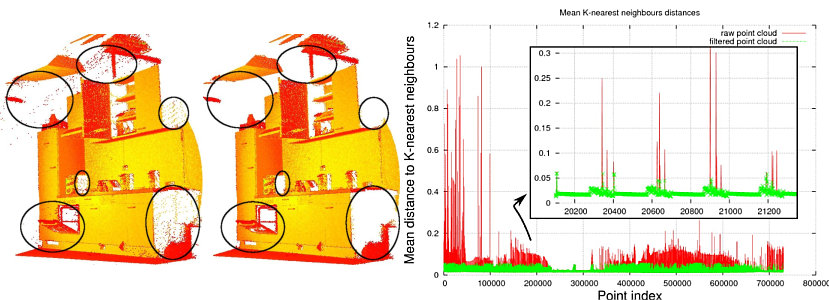
\includegraphics[width=\textwidth]{localization-system/statistical-outlier-removal}
	\caption[Statistical outlier removal filter]{Statistical outlier removal filter\protect\footnotemark}
	\label{fig:localization_system_statistical-outlier-removal}
\end{figure}
\footnotetext{\url{http://pointclouds.org/documentation/tutorials/statistical_outlier.php}}
%}


\subsection{Surface and object reconstruction and resampling}\label{subsec:localization_system_surface-reconstruction-resampling}

Depending on the level of sensor noise and amount of outliers present in a given point cloud, it may be necessary to employ surface reconstruction techniques to fill gaps in sensor data or correct measurements errors.

Moving least squares \cite{Alexa2003} is a surface reconstruction algorithm that uses higher order bivariate polynomials to fit surfaces to a given set of points. It can be used to fill possible gaps in sensor data, smooth the point cloud (shown in \cref{fig:localization_system_mls-smoothing}), refine surface normals (shown in \cref{fig:localization_system_mls-nomal-refinement}) and perform downsampling or upsampling.

Surface reconstruction can also be useful when the point cloud is built from several ambient scans with different origins and registered with some alignment errors. In \cref{fig:localization_system_mls-nomal-refinement} can be seen that the normal estimation is not very accurate in the overlapping regions between different scans. This can be solved by estimating the normals using the surfaces computed by the moving least squares algorithm instead of using the point's neighbors.


%\afterpage{
\begin{figure}[H]
	\centering
	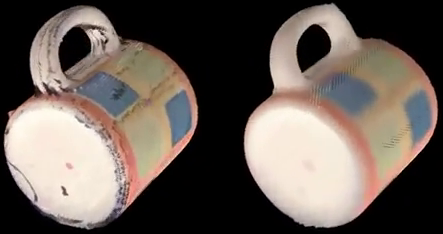
\includegraphics[width=0.57\textwidth]{localization-system/mls-smoothing}
	\caption[Surface smoothing using moving least squares algorithm]{Surface smoothing using moving least squares algorithm\protect\footnotemark}
	\label{fig:localization_system_mls-smoothing}
\end{figure}
\footnotetext{\url{http://pointclouds.org/documentation/tutorials/resampling.php}}
%}

%\afterpage{
\begin{figure}[H]
	\centering
	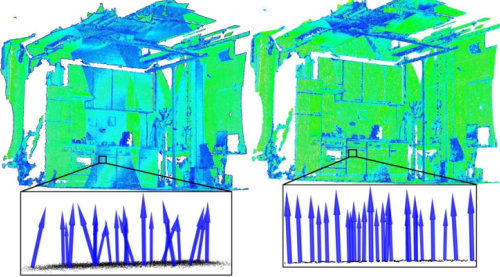
\includegraphics[width=0.57\textwidth]{localization-system/mls-nomal-refinement}
	\caption[Surface normals refinement using moving least squares algorithm]{Surface normals refinement using moving least squares algorithm \cite{Rusu2010a}}
	\label{fig:localization_system_mls-nomal-refinement}
\end{figure}
%}



\section{Normal estimation}

Most of feature detection, description and matching algorithms along with some registration methods rely on the point's surface normal and curvature. These algorithms analyze the neighborhood of a given point in order to compute the line / surface normal, and as such, the correct specification of what points should be included in the estimation is crucial to achieve accurate results. This depends on the environment geometry and the level of detail that is required, and is usually done by specifying a radius distance (example in \cref{fig:localization_system_surface-normals}) or by limiting the number of neighboring points to use.

The next sections describe some of the methods that are supported for 3/6 \gls{dof} sensor data.


\subsection{Line normal estimation}

Line normals give information about the spatial disposition and orientation of a given cluster of collinear points. They can be computed using \gls{ransac} methods \cite{Fischler1981} and their orientation can be corrected using the sensor's origin.


\subsection{Surface normal estimation}

Surface normals provide information about the orientation of the underlying geometry of a given point cluster. They can be computed using plane fitting methods or using more advanced techniques such as \gls{pca} \cite{Jolliffe2002} or the one presented in \cref{subsec:localization_system_surface-reconstruction-resampling}.

\begin{figure}[H]
	\centering
	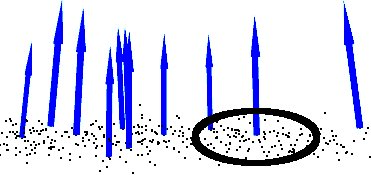
\includegraphics[width=0.5\textwidth]{localization-system/surface-normals}
	\caption[Point neighborhood for normal estimation]{Point neighborhood for normal estimation \cite{Rusu2010a}}
	\label{fig:localization_system_surface-normals}
\end{figure}



\section{Keypoint detection}

Keypoint detection aims to find interesting points in a given point cloud in order to compute the cloud registration faster or to perform feature description and matching. There are several approaches to find keypoints that have different definitions of what kind of points are worth analyzing. But they all should be able to detect the same keypoints given similar data and they aim to select the points that best describe the underlying point cloud geometry. Currently the localization system can use the Scale Invariant Feature Transform (SIFT) [17] algorithm on the points curvature or the Intrinsic Shape Signatures (ISS3D) [18] keypoint detector.


Aligning two point clouds with overlapping views of the environment requires the establishment of point correspondences. If both point clouds have similar sensor origins, these can be determined with nearest neighbor's searches and filtered with correspondence rejectors (using other point properties such as reflectance and color). But if they were acquired in two very different positions, then more advanced techniques must be employed.

One of those techniques uses histograms to describe the geometric properties of the environment around a given point. This allows points to be matched even if they have completely different Euclidean coordinates. Also, by using histograms and sampling techniques, these descriptors are much more robust against sensor noise and varying level of point density. However, these advantages come with a heavy computational cost, and as such, point descriptors should only be computed on the most descriptive areas of the environment.

Identifying these environment points is known as feature / keypoint detection, and usually involves finding interesting points, such as corners and edges. Besides uniqueness, these points must also be repeatable. This means that the detection algorithms should be able to find the same points even if they are present in different point clouds with sensor noise and varying point density. This is of the utmost importance, because if the same keypoints are not identified on both clouds, then matching the point descriptors will likely fail.

The next sections introduce some of the most used algorithms for normal estimation, keypoint detection and point description.


\subsection{Intrinsic Shape Signatures}

FF.


\subsection{SIFT keypoints}

FF.



\section{Keypoint description}

Describing a keypoint usually involves analyzing its neighboring points and computing a given metric or histogram that quantifies the neighbor’s relative distribution, their normals angular relation, associated geometry or other metrics that are deemed useful. Several approaches were suggested over the years according to different recognition needs and they are the basis of feature matching algorithms used in the initial pose estimation.

The localization system can use most of the keypoint descriptors available in PCL, namely the Point Feature Histogram (PFH), the Fast Point Feature Histogram (FPFH), the Signature of Histograms of Orientations (SHOT), the Shape Context 3D (SC3D), the Unique Shape Context (USC) and the Ensemble of Shape Functions (ESF).


\subsection{Point Feature Histograms}

FF.


\subsection{Fast Point Feature Histograms}

FF.


\subsection{Shape Context Estimation}

FF.


\subsection{Unique Shape context}

FF.


\subsection{SHOT estimation}

FF.


\subsection{Spin image estimation}

FF.


\subsection{Ensemble Shape Functions}

FF.


\subsection{Rotational Projection Statistics}

FF.


\section{Cloud registration}

Point cloud registration is the process of finding the transformation matrix (usually translation and rotation only) that when applied to a given ambient cloud will minimize an error metric (such as the mean square error of the ambient point cloud in relation to a given reference point cloud). Several approaches were suggested over the years and they can be categorized as point or feature cloud registration.



\section{Initial alignment with keypoint descriptors matching}

Feature registration is the process of matching keypoint descriptors in order to find an initial alignment between two point clouds. The proposed localization system uses a feature registration method similar to the Sample Consensus Initial Alignment algorithm presented in [20]. It uses a sample consensus approach to select the best registration transformation after a given number of iterations. In each iteration a subsample of randomly selected descriptors from the ambient cloud is retrieved. Then for each of these descriptors, k best matching descriptors in the reference point cloud are searched and one of them is chosen randomly (this improves robustness against noise in the sensor data and changes in the environment that are not yet integrated into the map). Later after having filtered these correspondences between ambient and reference descriptors, the registration matrix is computed. If this registration matrix results in a point cloud overlap that has a minimum of inliers percentage (a point in the ambient cloud is an inlier if it has a point in the reference cloud closer than a given distance), then it is considered an acceptable initial pose and is saved (to allow a localization supervisor to analyze the distribution of the acceptable initial poses). In the end of all iterations, the best initial pose (if found) is refined with a point cloud registration algorithm.



\section{Final alignment with point cloud error minimization}

Point cloud registration algorithms such as the Iterative Closest Point [19] (with its several known variations like ICP point-to-point, ICP point-to-point non-linear, ICP point-to-plane and generalized ICP) and the Normal Distributions Transform [6] are among the most popular algorithms to register point clouds. They can achieve very accurate cloud registration but they require an approximate initial pose for the registration to successfully converge to a correct solution (otherwise they may achieve only partial cloud overlap or even fail to converge to a valid solution). To solve this problem, a complete autonomous registration pipeline must also include the computation of this initial alignment through the usage of feature registration.


\subsection{Iterative Closest Point}

FF.


\subsection{Normal Distributions Transform}

FF.



\section{Outlier detection}

FF.




\section{Localization validation}

After a point cloud is registered, several metrics are calculated in order to evaluate if a valid pose can be retrieved using the registration matrix.

The first computed metrics are the percentage of inliers and the root mean square error of these inliers. If a minimum number of points was registered and the inlier percentage and root mean square error are acceptable, then the registration is considered successful. However, these registered points can be agglomerated in a small area and may not be representative of the robot location. As such, a second metric is computed that takes into account the angular distribution of these inliers. This metric gives a measurement of how reliable is this registration and is based on the fact that there is high confidence in a given estimation when there are correctly registered points all around the robot.

The last metrics are the corrections that the registration matrix introduced. Given that the localization system will be in tracking mode most of the time, it is possible to define how far a new pose can be in relation to the previous accepted location and discard new poses that exceed a given threshold. This is useful to discard pose corrections that are very unlikely to happen, such as the robot moving half a meter between poses when it is expected to move only at 30 cm/s. These situations can happen when there is a sudden decrease in the field of view (that can occur due to sensor occlusion or malfunction) or when  large unknown objects very similar to sections of the map appearinto the field of view of the robot.

If all these metrics are within acceptable thresholds, then the robot pose can be computed by applying the matrix correction to the initial pose associated with the ambient sensor data. If any of these metrics are not acceptable, then the system can be configured to simply discard this pose estimation and try to estimate the pose in the next sensor data update or it can apply a tracking recovery attempt with a different registration algorithm (or the same algorithm with different parameters). If several consecutive pose estimations are discarded, the system can have a second level of recovery that can be configured to use the initial pose estimation algorithms in order to finally estimate the robot pose and reset the tracking state.



\section{Dynamic map update}

After performing a successful pose estimation, the localization system can be paired with OctoMap [21] in order to update the localization map by either integrating only the unknown objects or the full registered point cloud. Integrating only the unknown objects is the recommended approach when there is a known map and the environment is expected to change gradually. This is also more efficient as only the points that need to be integrated are processed and ray traced in OctoMap. On the other hand, integrating the full registered cloud can be desirable if the map of the environment is very incomplete, very outdated or expected to change considerably during the operation of the robot.

\chapter{Localization system evaluation} \label{chap:localization-system-evaluation}



\section*{}

This chapter presents several test scenarios that were devised to evaluate the implemented localization system. They aim to test the accuracy and robustness of the implementation under different environmental conditions and hardware configurations.



\section{Testing platforms}

The localization system was tested on laser sensor data retrieved from three different mobile robot platforms and executed on the same computer in order to allow a direct comparison of computation time. This computer was a Clevo P370EM3 laptop (with a Intel Core i7 3630QM CPU at 2.4GHz, 16 GB of RAM DDR3, NVidia GTX680M graphics card and a Samsung 840 Pro SSD) and it was running Ubuntu 12.04 along with \gls{ros} Hydro, \gls{pcl} 1.7 and Gazebo 1.9.

The sensor data was recorded into rosbags, and is publicly available at\footnote{\url{https://github.com/carlosmccosta/dynamic_robot_localization_tests}} along with all the detailed results and experiments videos, in order to allow future comparisons with other localization systems. The hardware specifications of the \glspl{lidar} used is presented in \cref{tab:localization-system-evaluation_laser-hardware-specifications} and the laser points after downsampling and registration can be seen on the movement paths figures as green circles (inliers) and red circles (outliers).


\subsection{Jarvis platform}

The Jarvis platform is an autonomous ground vehicle equipped with a SICK NAV 350 laser for self-localization (mounted about 2 meters from the floor) and a SICK S3000 laser for collision avoidance (mounted about 0.20 meters from the floor). It uses a tricycle locomotion system with two back wheels and a steerable wheel at the front. In \cref{fig:localization-system-evaluation_jarvis} the robot is performing a delivery task with the package on top of a moving support. The 3 \gls{dof} ground truth was provided by the SICK NAV350 system and relied on 6 laser reflectors (with 9 cm of diameter) to perform the pose estimations (it is certified for robot docking operations with precision up to 4 millimeters).

\begin{figure}[H]
	\centering
	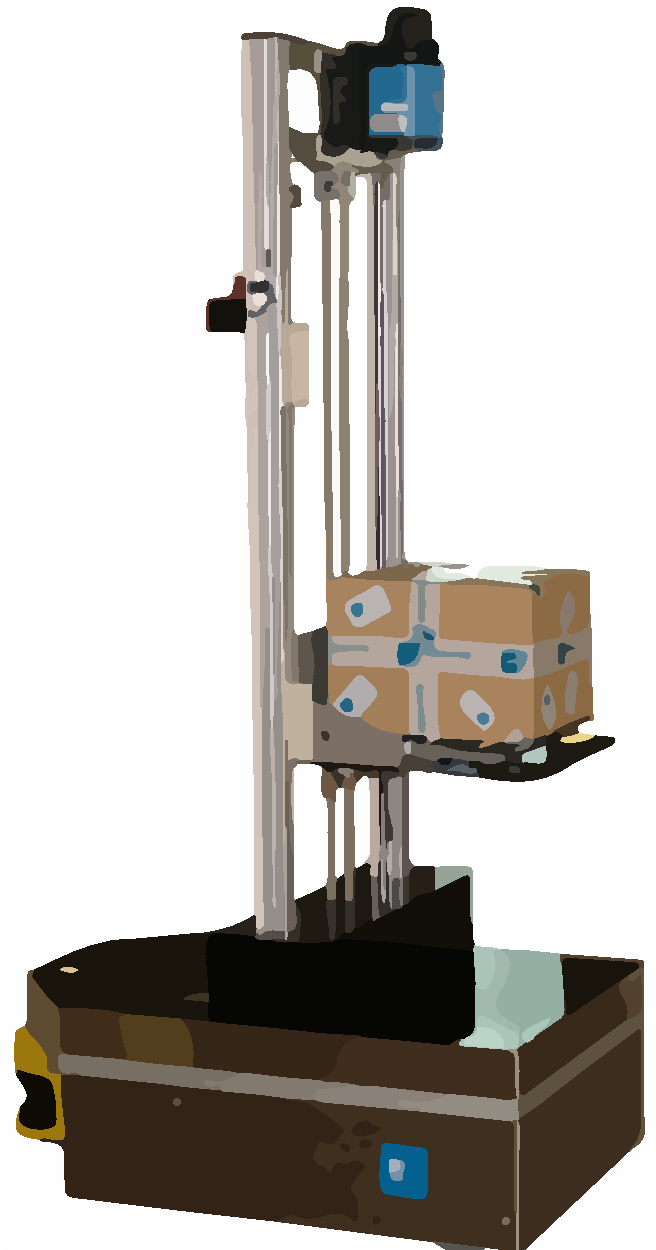
\includegraphics[width=0.28\textwidth]{localization-system-evaluation/testing-platforms/jarvis}
	\caption{Jarvis testing platform}
	\label{fig:localization-system-evaluation_jarvis}
\end{figure}


\subsection{Pioneer 3-DX platform}

The Pioneer 3-DX shown in \cref{fig:localization-system-evaluation_pioneer} is a small lightweight robot equipped with a SICK LMS-200 laser (mounted about 48 cm from the floor) and a Kinect (mounted about 78 cm from the floor). It uses a two-wheel two-motor differential drive locomotion system and can reach a linear speed of 1.2 m/s and angular velocity of 300º/s. The 3 \gls{dof} ground truth was provided by 8 Raptor-E cameras \footnote{\url{http://www.motionanalysis.com/html/movement/raptore.html}} and according to \cite{Sturm2012} it had less than 1 cm in translation error and less than 0.5 degrees in rotation error.

\begin{figure}[H]
	\centering
	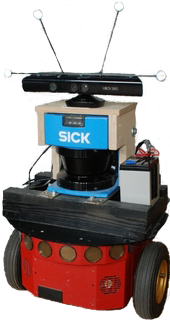
\includegraphics[width=0.25\textwidth]{localization-system-evaluation/testing-platforms/pioneer-3dx}
	\caption{Pioneer 3-DX testing platform \cite{Sturm2012}}
	\label{fig:localization-system-evaluation_pioneer}
\end{figure}


\subsection{Guardian platform}

The Guardian platform is an autonomous mobile manipulator equipped with a Hokuyo URG-04LX laser in the front and a Hokuyo URG-04LX\_UG01 laser in the back (both mounted about 0.37 meters from the ground). The front laser had a tilting platform which allows 3D mapping of the environment. The arm is a SCHUNK Powerball LWA 4P and in \cref{fig:localization-system-evaluation_guardian} it is attached to a stud welding machine (in simulation it is attached to a video projector). It uses a differential drive locomotion system and can be moved with wheels or with tracks. This platform didn't have a certified ground truth and as such, the results could not be quantified with an external localization system (the results performed with the Gazebo simulator will be presented instead - robot model shown in \cref{fig:localization-system-evaluation_guardian_gazebo}).

\begin{figure}[H]
	\centering
	\begin{minipage}[h]{0.497\textwidth}
		\centering
		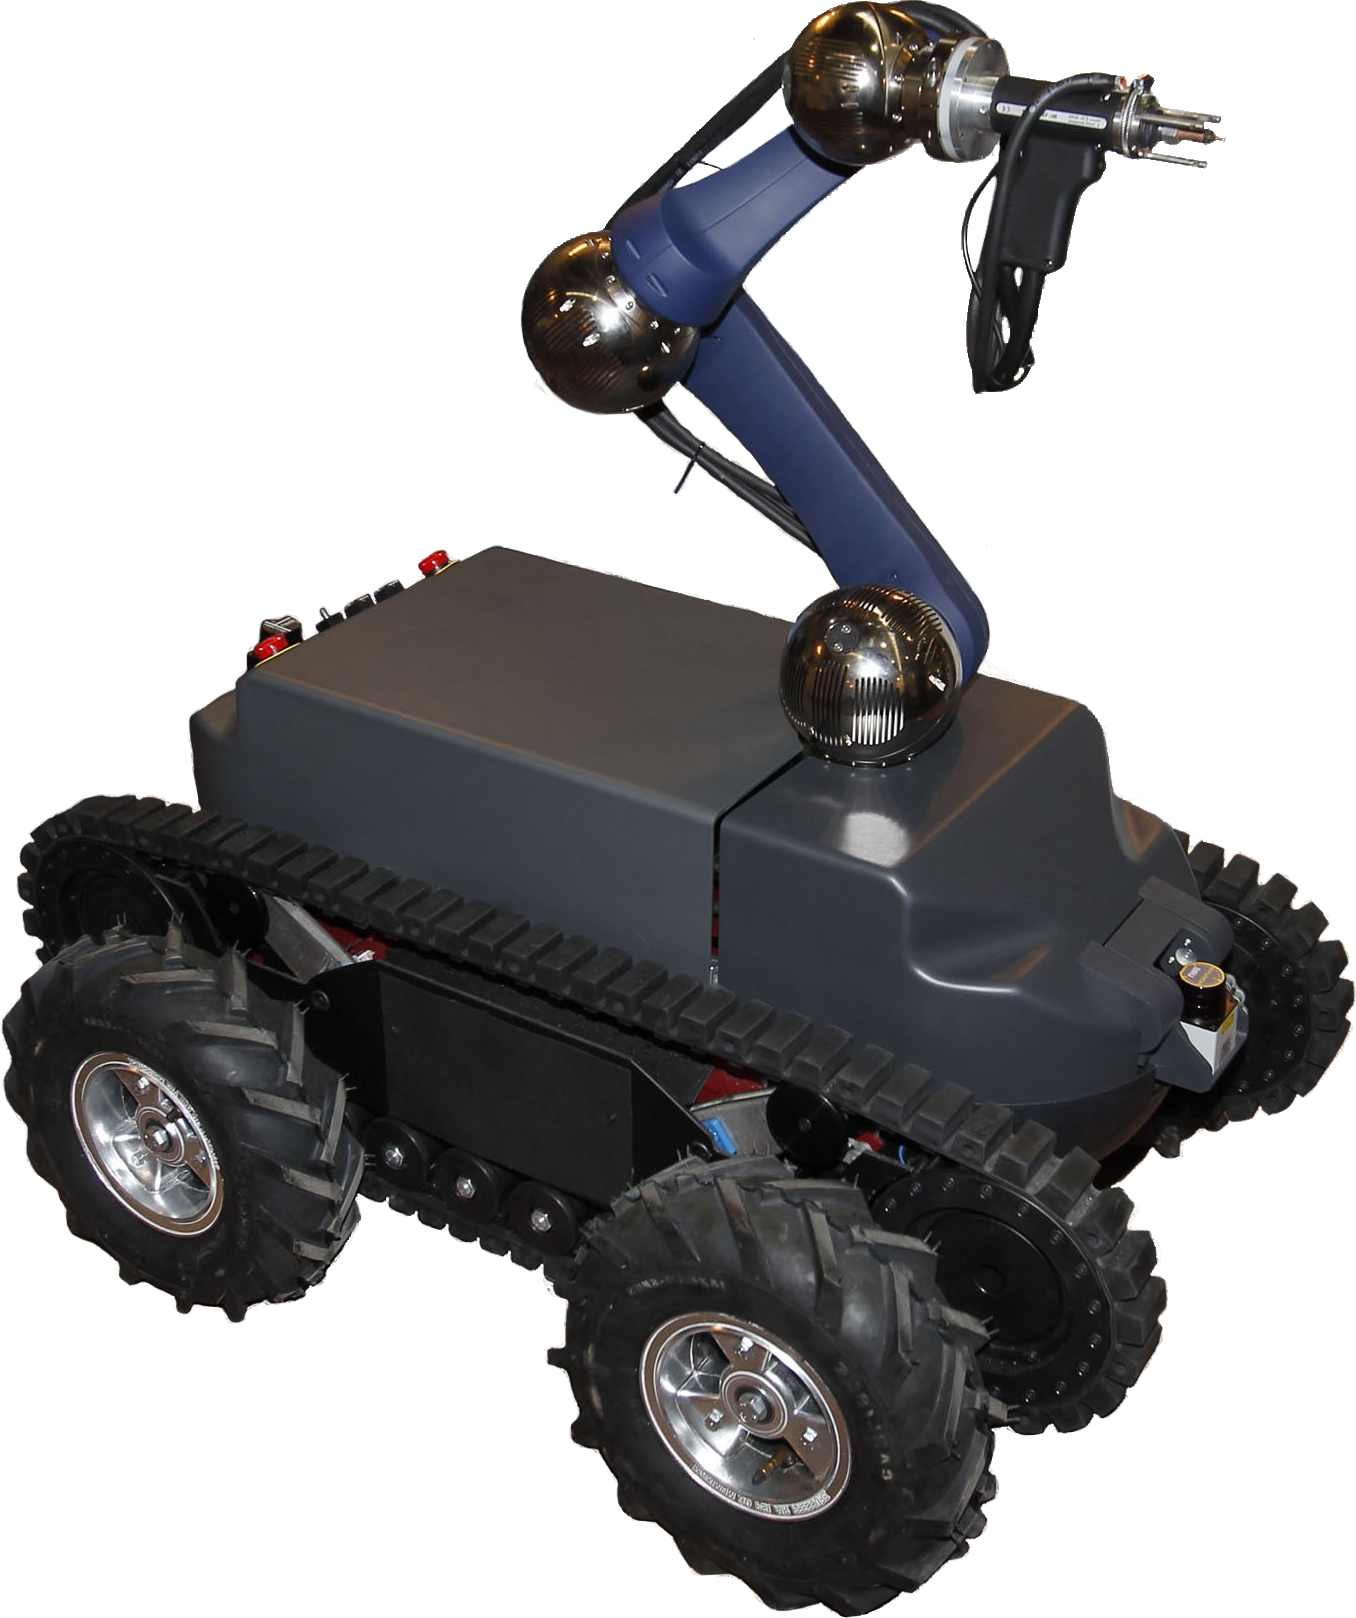
\includegraphics[width=0.7\textwidth]{localization-system-evaluation/testing-platforms/guardian}
		\caption{Guardian testing platform}
		\label{fig:localization-system-evaluation_guardian}
	\end{minipage}\hfill
	\begin{minipage}[h]{0.497\textwidth}
		\centering
		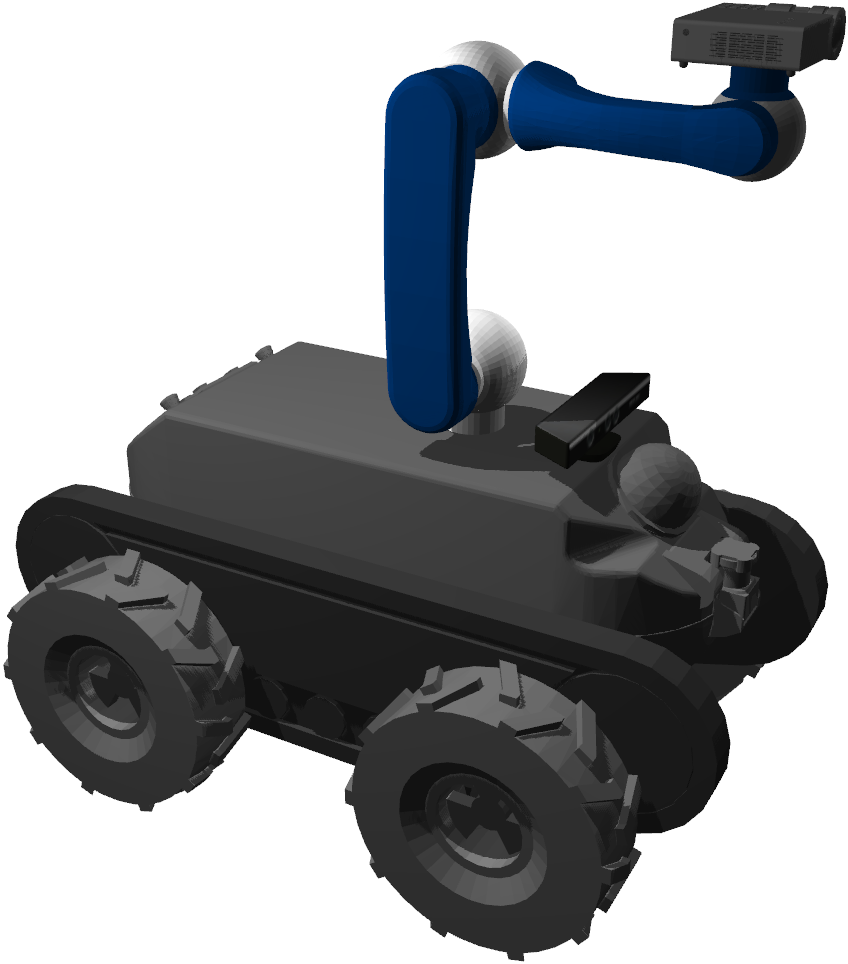
\includegraphics[width=0.7\textwidth]{localization-system-evaluation/testing-platforms/guardian-gazebo}
		\caption{Guardian Gazebo simulation}
		\label{fig:localization-system-evaluation_guardian_gazebo}
	\end{minipage}
\end{figure}


\begin{table}[H]
	\caption{\glsentryplural{lidar} hardware specifications}
	\tabulinesep = 0.8ex
	\centering
	\small
	\begin{tabu} { X[2.5,m,c] | X[m,c] X[m,c] X[m,c] X[m,c] X[m,c] }
		\rowfont{\bfseries\itshape} Laser model & Range (meters) & Field of view (degrees) & Scanning frequency (Hz) & Angular resolution (degrees) & Statistical error (millimeters) \\
		\hline
		{\small SICK NAV350} 			& [0.5..250] 	& 360 	& 8 	& 0.25 	& 15 	\\
		{\small SICK S3000} 			& [0.1..49] 	& 190 	& 8 	& 0.25 	& 150 	\\
		{\small SICK LMS200} 			& [0.1..80] 	& 180 	& 10 	& 1.0 	& 35 	\\
		{\small Hokuyo URG-04LX} 		& [0.06..4.095] & 240 	& 10 	& 0.36 	& 10 	\\
		{\small Hokuyo URG-04LX\_UG01} 	& [0.02..4] 	& 240 	& 10 	& 0.36 	& 30 	\\
	\end{tabu}
	\label{tab:localization-system-evaluation_laser-hardware-specifications}
\end{table}


\section{Testing environments}

The localization system was tested in different environments and used the Jarvis platform in a large room with a RoboCup field, the Pioneer 3-DX in a large industrial hall, the Guardian platform in a simulated indoor environment and a Kinect in a flying arena.


\subsection{Jarvis in RoboCup field}

The RoboCup field (shown in \cref{fig:localization-system-evaluation_jarvis-tests-environment}) occupies half of a large room (with 20.5 meters of length and 7.7 meters of depth). It has two doors, several small windows and two large glass openings into the hallway. Several tests were performed with the robot at speeds ranging from 5 cm/s to 50 cm/s in this environment and up to 2 m/s using the Stage simulator\footnote{\url{http://rtv.github.io/Stage/}}. These tests were performed with two different movement paths. The first is a simple rounded path (shown in \cref{subsec:appendix-a_jarvis-robot-tests_rounded-path-using-the-jarvis-robot-at-5-cm-s,subsec:appendix-a_jarvis-robot-tests_rounded-path-using-the-jarvis-robot-at-30-cm-s}) that aimed to test the robot in the region of space that had better ground truth (due to its position in relation to the laser reflectors). The second path was more complex and contained several sub paths with different velocities and shapes (shown from \crefrange{subsec:appendix-a_jarvis-robot-tests_complex-path-using-the-jarvis-robot-at-5-cm-s}{subsec:appendix-a_jarvis-robot-tests_complex-path-using-the-jarvis-robot-at-50-30-50-10-cm-s-without-laser-spherical-linear-interpolation}). It was intended to evaluate the localization system with typical movements that mobile manipulators require, such as moving forward and backwards with or without angular velocity and stopping at the desired destination.


\begin{figure}[H]
	\centering
	\begin{subfigure}[h]{.497\textwidth}
		\centering
		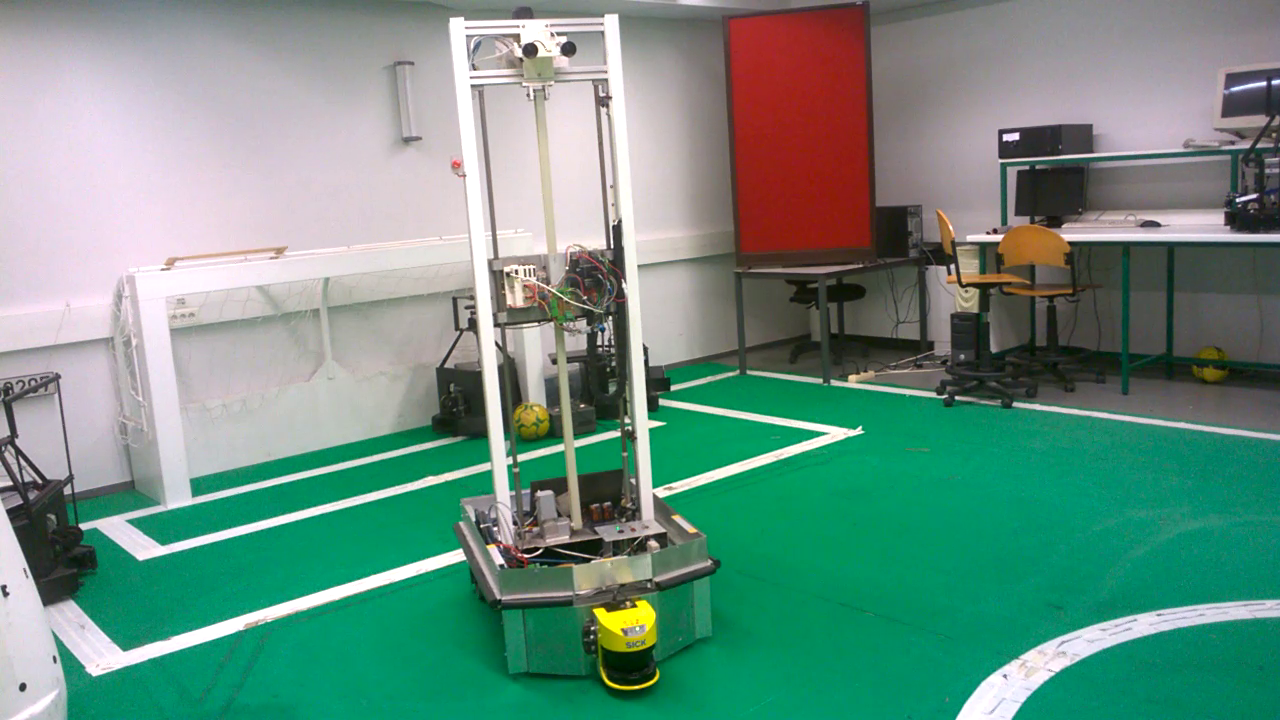
\includegraphics[width=\textwidth]{localization-system-evaluation/testing-environments/jarvis-environment-front-left}
	\end{subfigure}
	\begin{subfigure}[h]{.497\textwidth}
		\centering
		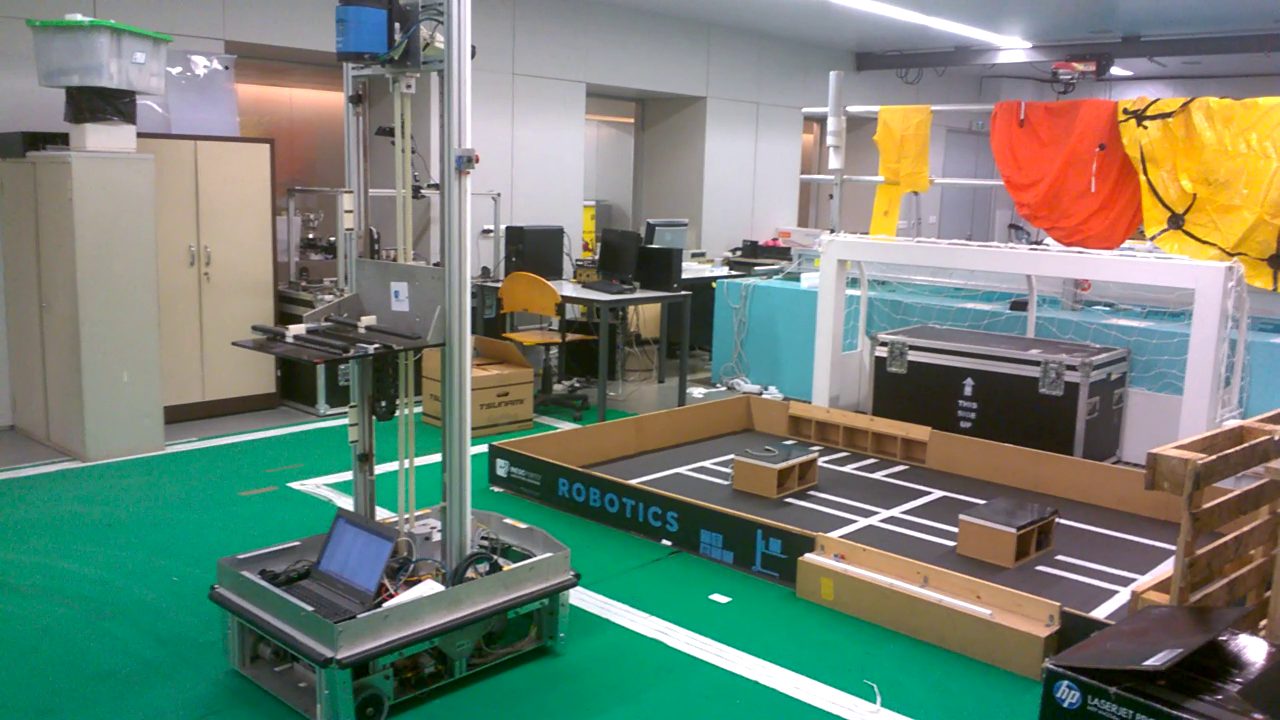
\includegraphics[width=\textwidth]{localization-system-evaluation/testing-environments/jarvis-environment-front-right}
	\end{subfigure}
	\caption{Jarvis testing environment}
	\label{fig:localization-system-evaluation_jarvis-tests-environment}
\end{figure}


\subsection{Guardian in structured environment}

The structured environment simulated in Gazebo is a large room with 12.4 meters of length and 8.4 meters of depth. It has 4 doors, several small windows and the walls have small ledges at regular intervals (as can be seen from \crefrange{fig:localization-system-evaluation_guardian-tests-environment}{fig:localization-system-evaluation_guardian-tests-environment-interactive}).

Given that the Guardian mobile manipulator is expected to work on the walls of this environment, several tests were devised with a path following the lower and right wall of the environment (shown from \crefrange{subsec:appendix-a_guardian-simulator-tests_wall-following-path-using-the-simulated-guardian-robot-at-30-cm-s-in-static-environment}{subsec:appendix-a_guardian-simulator-tests_wall-following-path-using-the-simulated-guardian-robot-at-30-cm-s-in-dynamic-cluttered-environment}). The first test was done in a static environment clear of unknown objects and was meant to evaluate the best precision that the localization system could achieve. The second test was done in a cluttered environment and was designed to test the robustness of the localization system against static unknown objects, that were placed in the middle of the environment and close to the walls (to block sensor data from reaching known positions and analyze the robustness of matching unknown points that are close to known areas). The last test added a moving car to the scene and aimed to assess the impact of dynamic objects on the point cloud registration algorithms.


\begin{figure}[H]
	\centering
	\begin{subfigure}[h]{.497\textwidth}
		\centering
		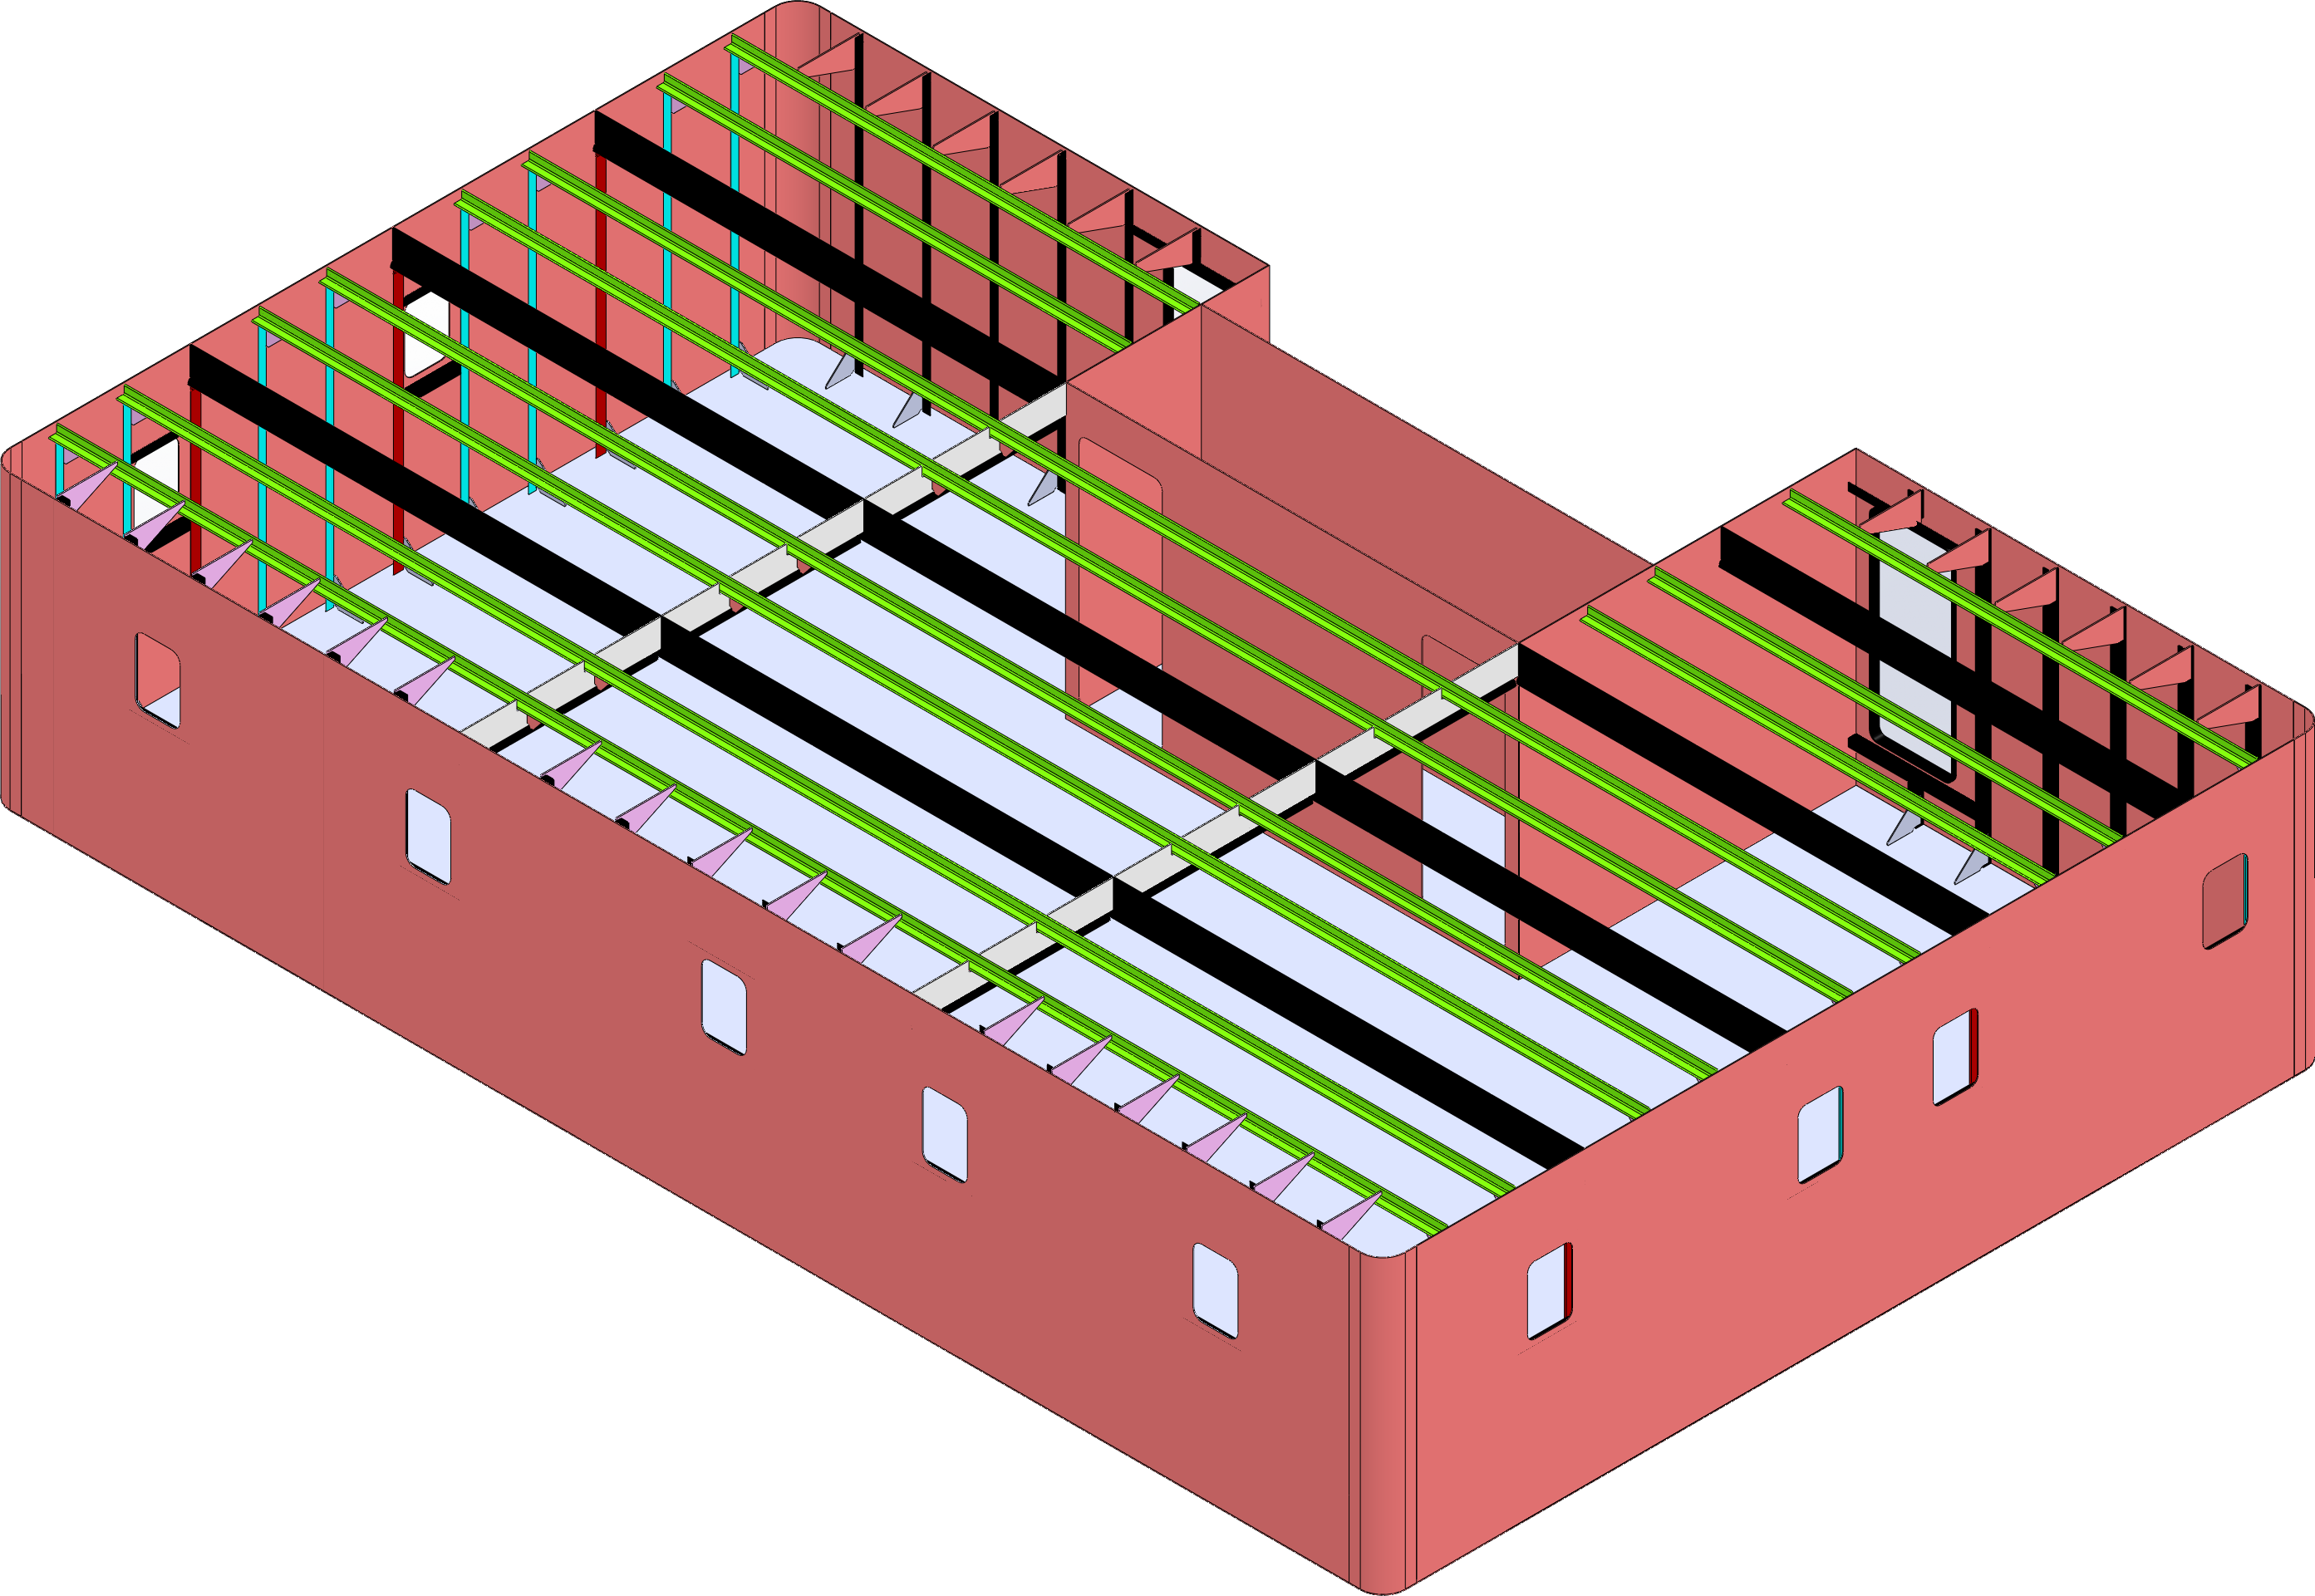
\includegraphics[width=\textwidth]{localization-system-evaluation/testing-environments/guardian-environment-corner}
	\end{subfigure}
	\begin{subfigure}[h]{.497\textwidth}
		\centering
		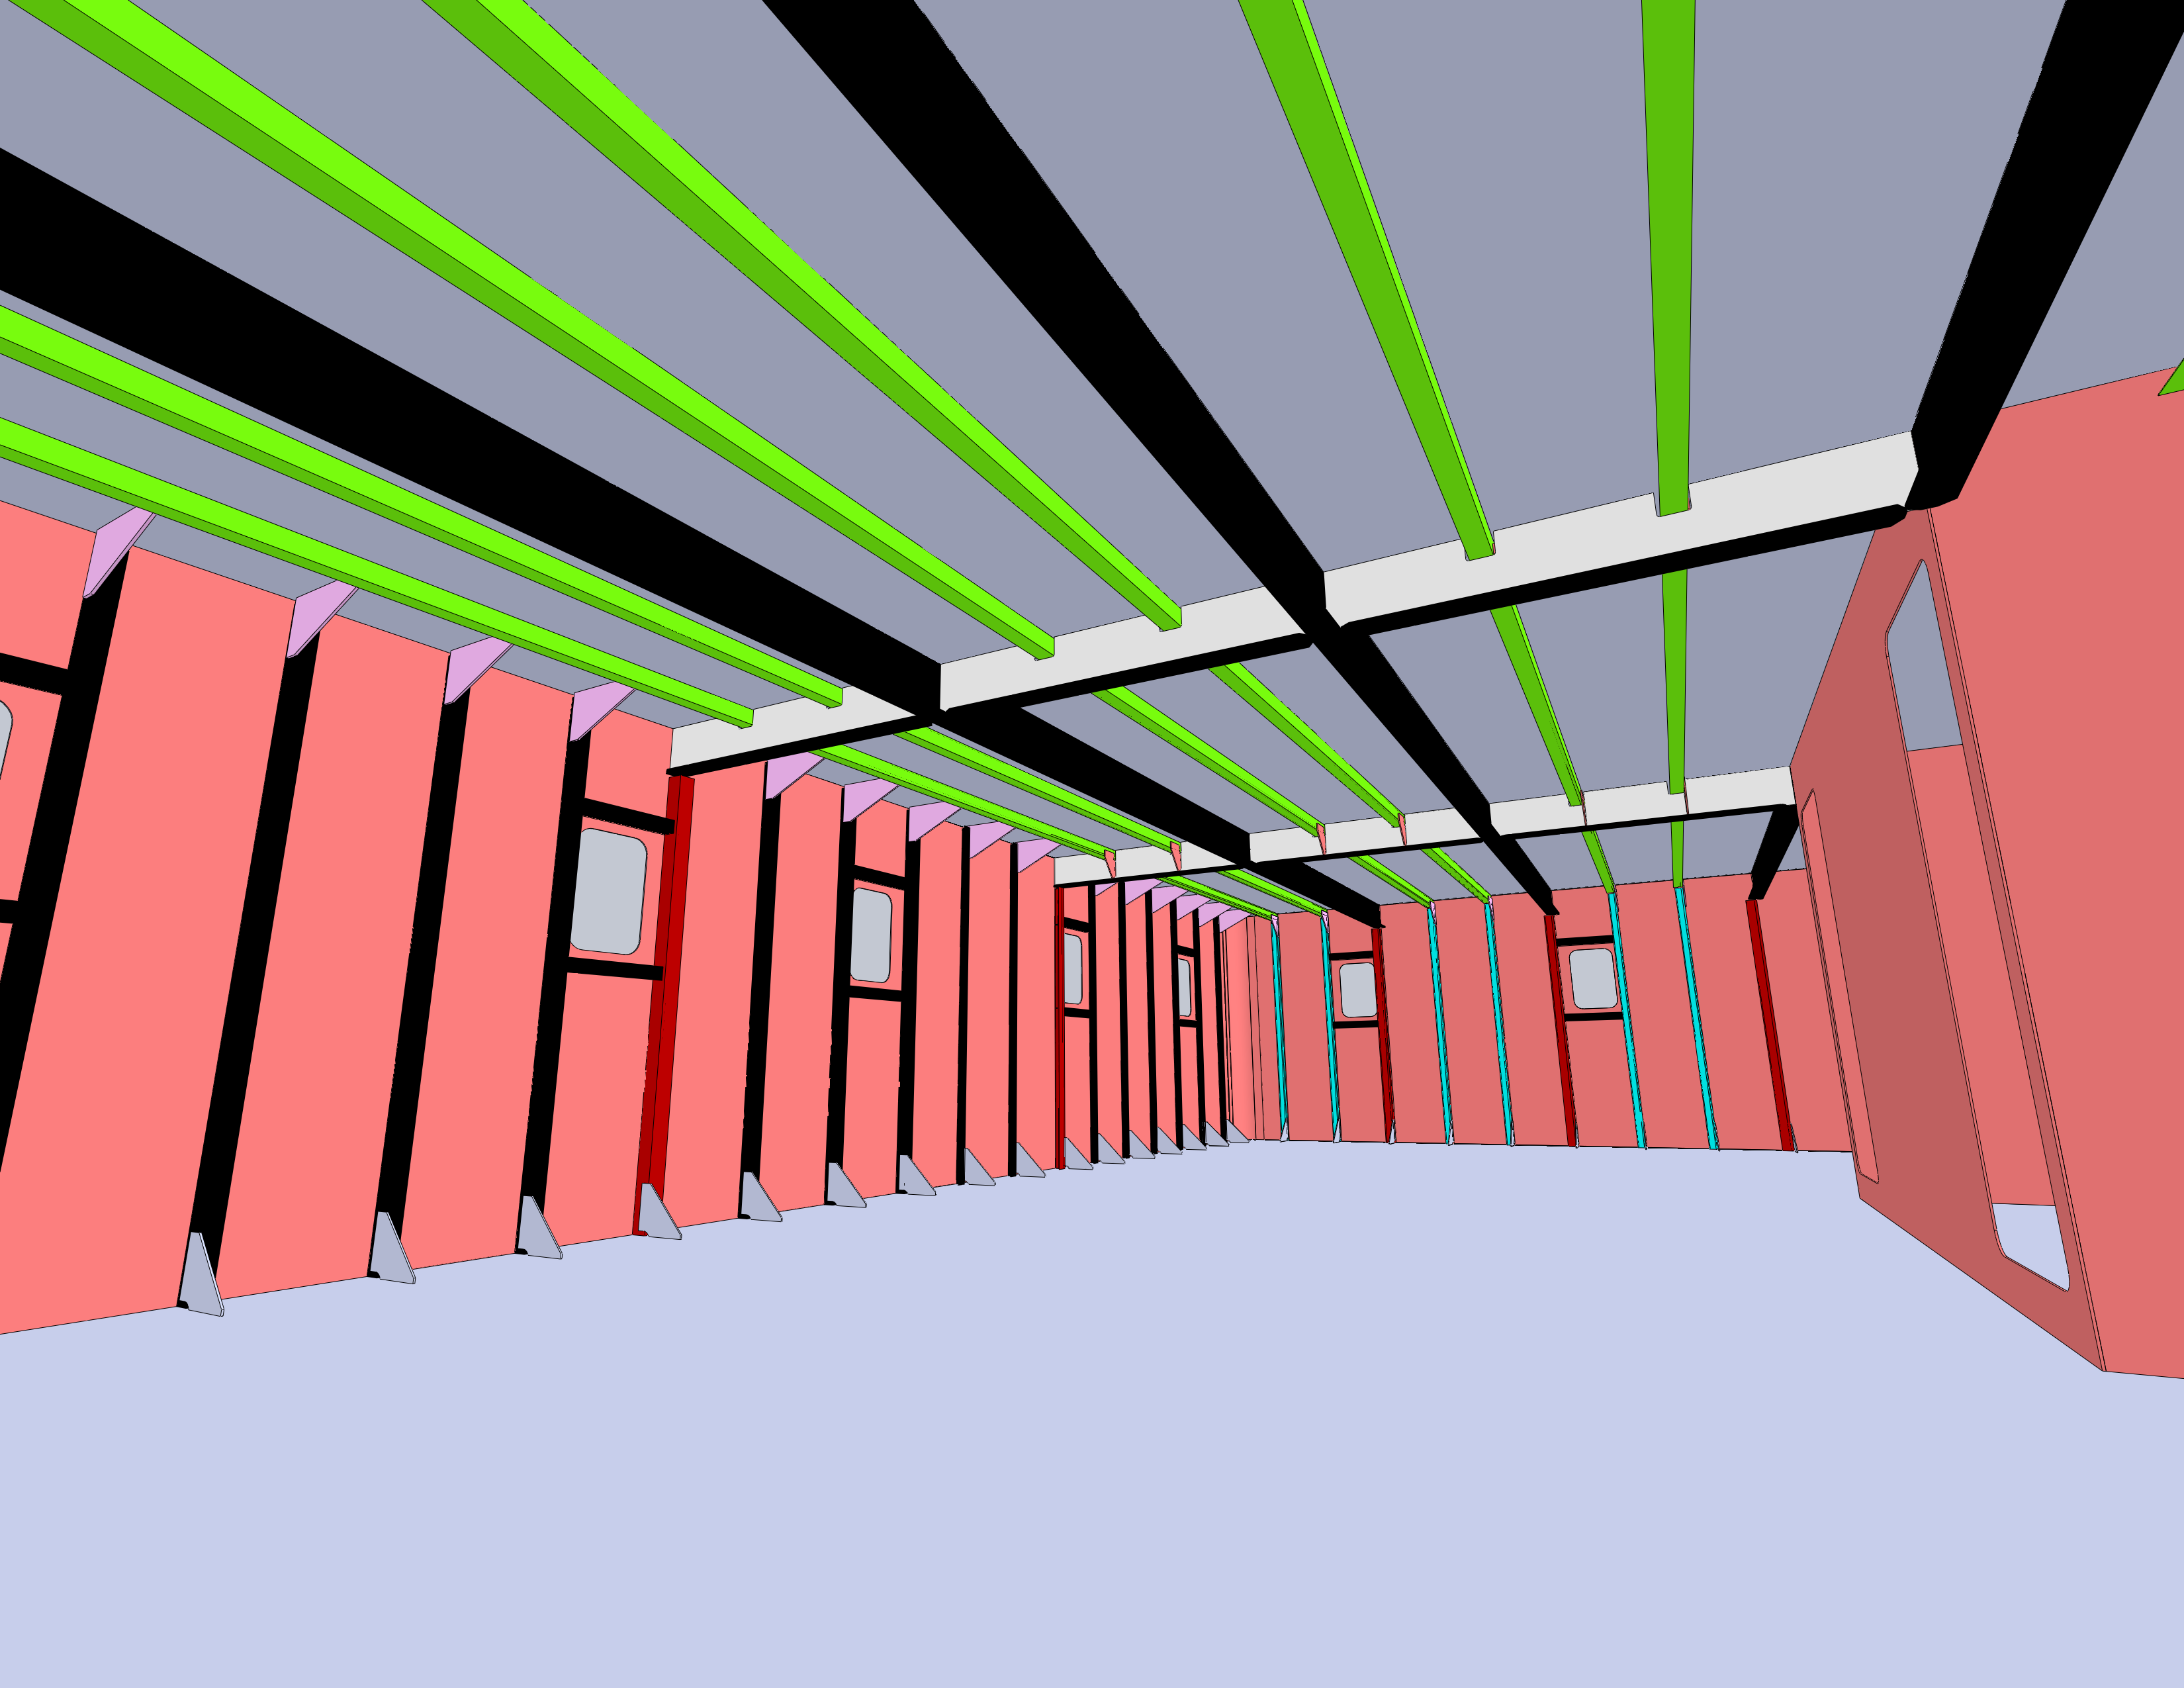
\includegraphics[width=\textwidth]{localization-system-evaluation/testing-environments/guardian-environment-inside}
	\end{subfigure}
	\caption{Guardian testing environment}
	\label{fig:localization-system-evaluation_guardian-tests-environment}
\end{figure}

\begin{figure}[H]
	\centering
	\begin{subfigure}[h]{.497\textwidth}
		\centering
		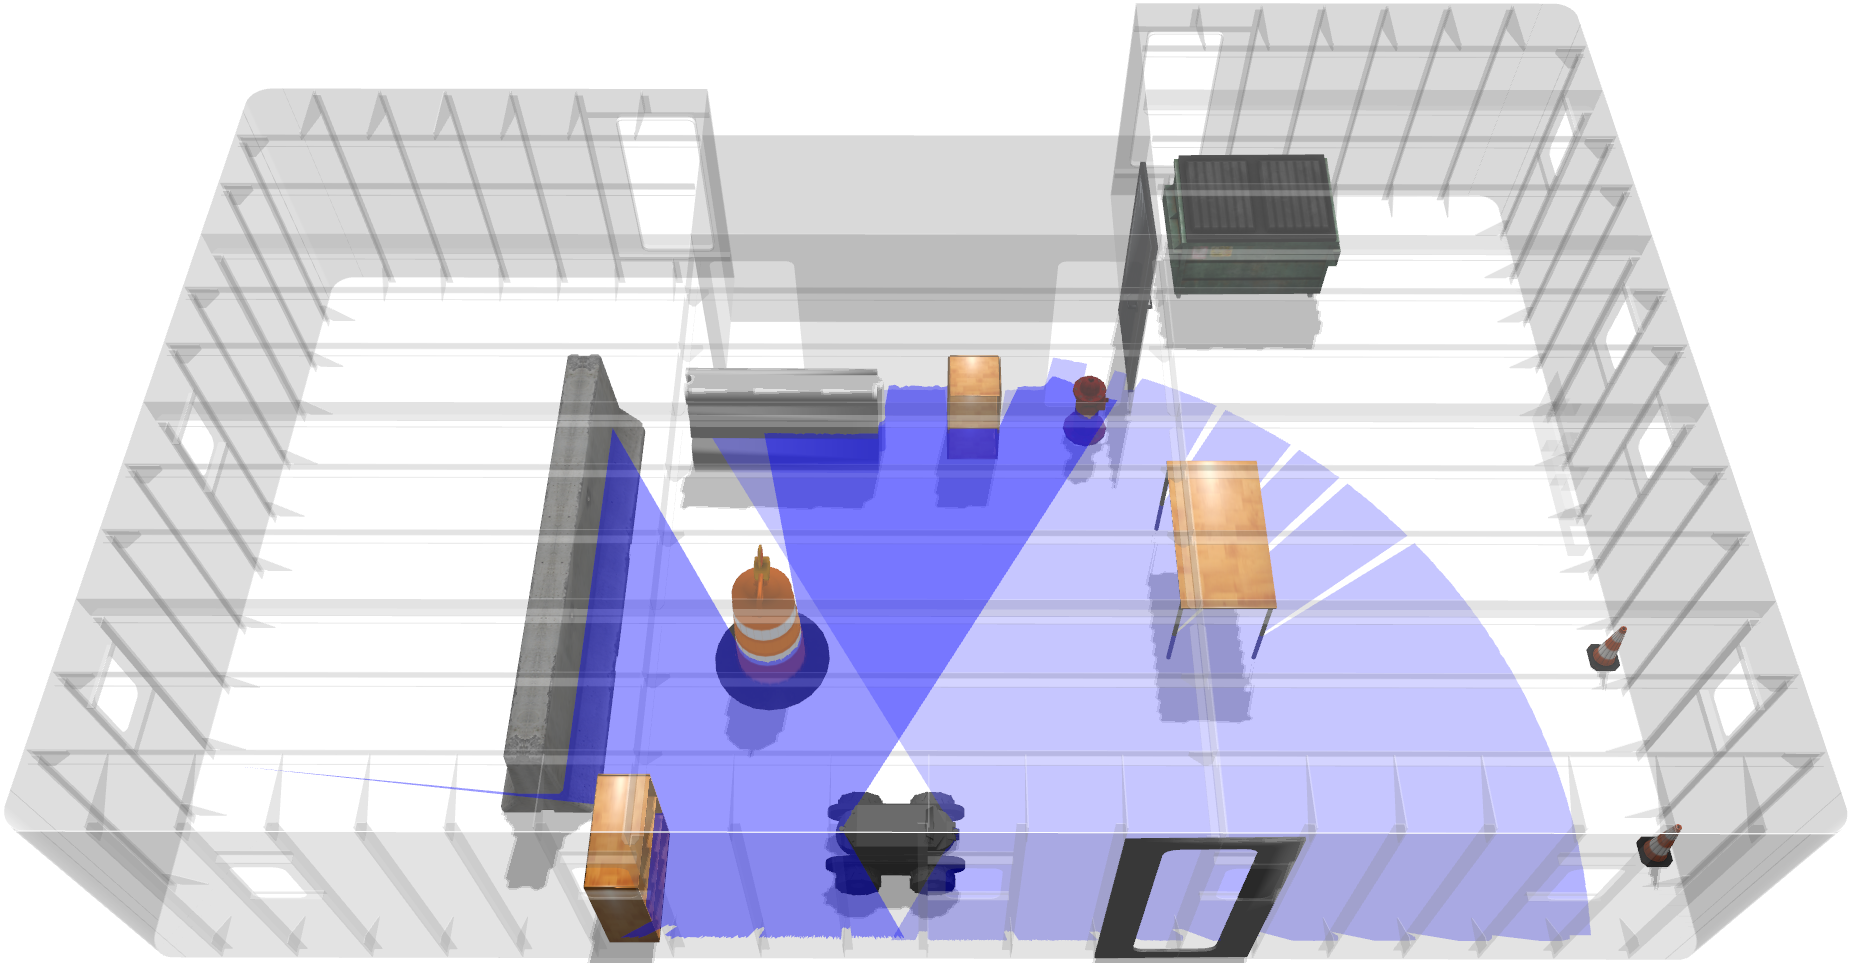
\includegraphics[width=\textwidth]{localization-system-evaluation/testing-environments/guardian-environment-cluttered}
	\end{subfigure}
	\begin{subfigure}[h]{.497\textwidth}
		\centering
		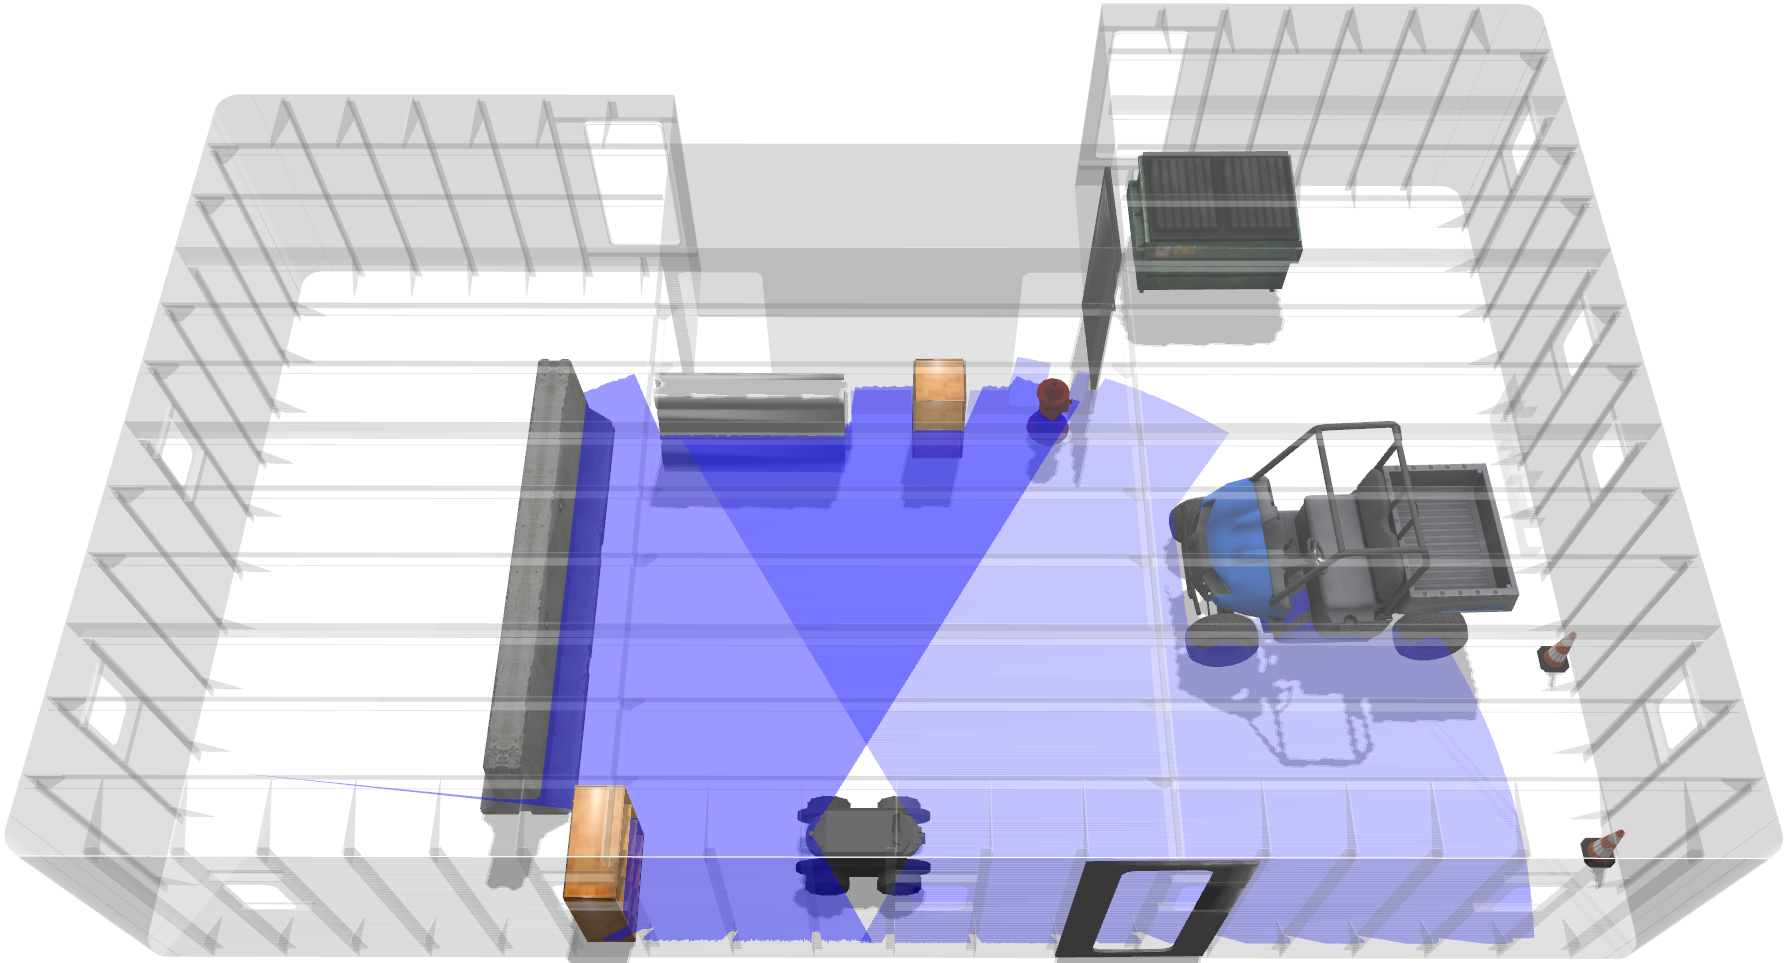
\includegraphics[width=\textwidth]{localization-system-evaluation/testing-environments/guardian-environment-cluttered-dynamic}
	\end{subfigure}
	\caption{Guardian cluttered (left) and dynamic (right) testing environment}
	\label{fig:localization-system-evaluation_guardian-tests-environment-cluttered}
\end{figure}

\begin{figure}[H]
	\centering
	\includemedia[
		label=guardian-environment,
		3Dviews=figures/localization-system-evaluation/testing-environments/guardian-environment.vws,
		width=\linewidth,
		height=0.6\linewidth,
		activate=pageopen,3Dtoolbar,3Dmenu
	]{}{figures/localization-system-evaluation/testing-environments/guardian-environment.u3d}
	\caption{Interactive \glsentrytext{cad} of Guardian testing environment (.u3d file)}
	\label{fig:localization-system-evaluation_guardian-tests-environment-interactive}
\end{figure}



\subsection{Pioneer in industrial hall}

The industrial hall is a large room with several tables and objects spread around. Four tests were performed with the Pioneer in this environment. The first was a 360º path with few objects in the middle of the room, while the remaining 3 were done with a lot of large objects, that significantly reduced the field of view of the robot laser (as can be seen in \cref{fig:localization-system-evaluation_industrial-hall}).

\begin{figure}[H]
	\centering
	\begin{subfigure}[h]{.497\textwidth}
		\centering
		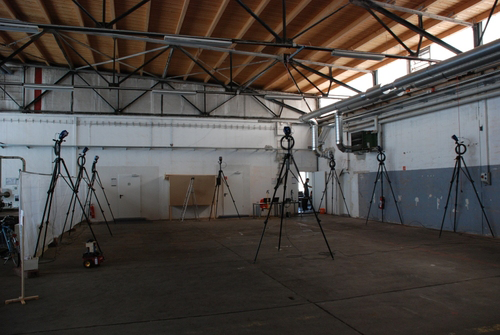
\includegraphics[width=0.95\textwidth]{localization-system-evaluation/testing-environments/industrial-hall-1}
	\end{subfigure}
	\begin{subfigure}[h]{.497\textwidth}
		\centering
		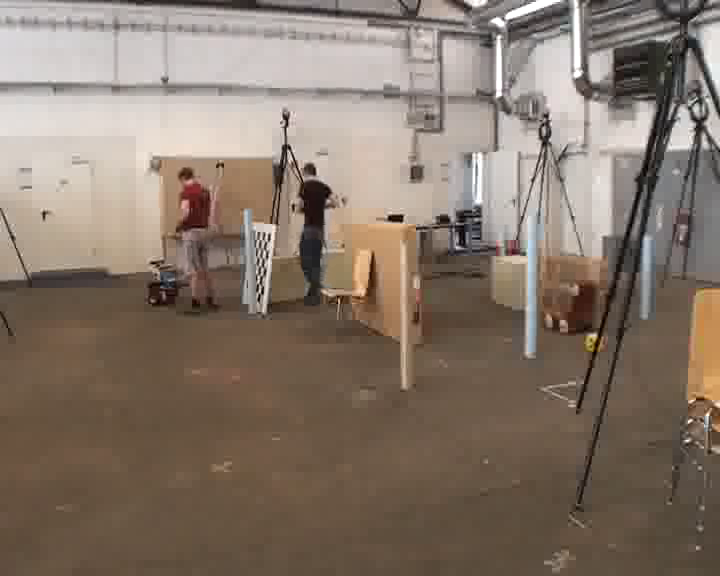
\includegraphics[width=0.8\textwidth]{localization-system-evaluation/testing-environments/industrial-hall-2}
	\end{subfigure}
	\caption{Industrial hall with and without objects in the center \cite{Sturm2012}}
	\label{fig:localization-system-evaluation_industrial-hall}
\end{figure}



\subsection{Kinect in flying arena}

The flying arena shown in \cref{fig:localization-system-evaluation_flying-arena} is a large room in which several objects were added to test 6 \gls{dof} pose tracking. In these tests the Kinect was moved by the operator in three different paths. The first was a smooth fly movement over the testing scene, while the other two aimed to test paths with mainly translations and rotations. This environment had a ground truth provided by Vicon cameras and according to the authors of the dataset \cite{Pomerleau2011} it had sub-centimeter accuracy \footnote{\url{http://www.vicon.com/}}.

\begin{figure}[H]
	\centering
	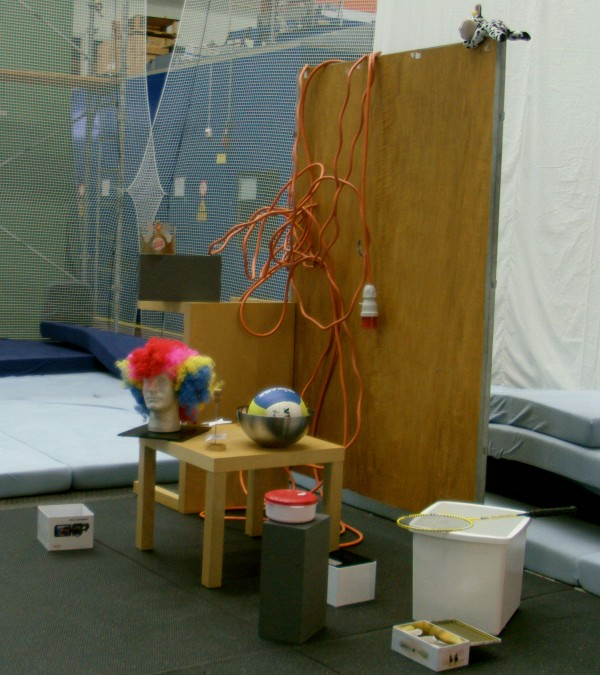
\includegraphics[width=0.4\textwidth]{localization-system-evaluation/testing-environments/kinect-flying-arena}
	\caption{Flying arena environment \cite{Pomerleau2011}}
	\label{fig:localization-system-evaluation_flying-arena}
\end{figure}




\section{3 \glsentrytext{dof} localization system tests}


\subsection{Overview}

The main results of the 3 \gls{dof} tests performed with the localization system are presented in \cref{tab:localization-system-evaluation_3-dof-results,tab:localization-system-evaluation_3-dof-results-odometry-amcl}. They summarizes each test by fitting a normal distribution for each evaluation metric. They were retrieved with a known initial pose and used \gls{icp} point-to-point as tracking algorithm and \gls{icp} point-to-plane as tracking recovery method. The Jarvis and Pioneer tests had a map built using the localization system in \gls{slam} mode and were manually corrected to achieve a resolution of 10 and 25 mm respectively. The Guardian tests relied on a map built from the \gls{cad} model with resolution of 2 mm. A voxel grid of 50 mm was applied to the assembled laser scans in order to reduce the impact of sensor measurement noise and also control the level of detail of the point clouds. The initial pose estimation subsystem used \gls{sift} for keypoint selection, \gls{fpfh} for keypoint description and the feature matching algorithm described in \cref{subsec:localization-system_feature-registration} to estimate the initial position and orientation of the robot (\cref{fig:localization-system-evaluation_ship-interior-initial-pose-estimation-sift-fpfh-ransac-gicp} shows the accepted initial poses when the robot was in the lower right corner of the Guardian test environment).

The next sections will provide an overview analysis of the main 3 \gls{dof} results achieved with the proposed localization system (available in \cref{app:appendix-a}). It will start by explaining how laser spherical interpolation can mitigate point cloud deformation. Later on it will analyze the point cloud preprocessing stage and why it should be carefully tuned to the sensors and ambient geometry. Next it will present the \gls{slam} problem and why it is necessary to have accurate maps in order to achieve precise localization. Finally it will be presented a global analysis of the tests, in which the results achieved by the proposed localization system will be compared with the ground truth, odometry and \gls{amcl}.

\clearpage

\begin{sidewaystable}
	\caption{3 \glsentrytext{dof} localization system results - (*) Most relevant experiments}
	\tabulinesep = 1.2ex
	\setlength{\tabcolsep}{0.2em}
	\centering
	\tiny
	\begin{tabu} to \textwidth { X[m,c] X[m,c] X[m,c] X[m,c] X[1.7m,c] X[m,c] X[m,c] X[0.01m,c] X[m,c] X[m,c] X[0.01m,c] X[m,c] X[m,c] X[0.01m,c] X[m,c] X[m,c] X[0.01m,c] X[m,c] X[m,c] }
		\hline
		\multicolumn{7}{c}{Test conditions} && \multicolumn{2}{c}{Translation error (millimeters)} && \multicolumn{2}{c}{Rotation error (degrees)} && \multicolumn{2}{c}{Outliers percentage [0..100]} && \multicolumn{2}{c}{Global computation time (milliseconds)} \\
		\cline{1-7} \cline{9-10} \cline{12-13} \cline{15-16} \cline{18-19}
		Section 	& Platform 																& Ambient 													& Path shape 											& Path velocities 		& Map cell resolution 	& Nº scans / Nº lasers 	&& Mean   & Standard deviation 	&& Mean  & Standard deviation 	&& Mean  & Standard deviation 	&& Mean   & Standard deviation \\ \hline
		A.1.1		& \multirow{4}{0.05\textwidth}{\centering Jarvis robot} 				& \multirow{2}{0.05\textwidth}{\centering Cluttered} 		& \multirow{2}{0.05\textwidth}{\centering Rounded} 		& 5 cm/s 				& 10 mm					& 1-4/1 				&& 3.384  & 1.900 				&& 0.549 & 0.087 				&& 15.75 & 3.84 				&& 12.052 & 12.232	\\
		A.1.2		&																		&															&														& 30 cm/s				& 10 mm					& 1-4/1					&& 12.250 & 8.901				&& 0.535 & 0.414				&& 16.08 & 3.80					&& 21.295 &	8.352	\\ \tabucline[0.5pt on 3pt off 2pt]{3-4}
		A.1.3		&																		& \multirow{2}{0.05\textwidth}{\centering Cluttered dynamic}& \multirow{2}{0.05\textwidth}{\centering Complex} 		& 5 cm/s 				& 10 mm					& 1-4/1			 		&& 4.280  & 2.264 				&& 0.441 & 0.070 				&& 24.35 & 5.17 				&& 11.776 & 12.265	\\
		A.1.4 (*)	&																		&															&														& {50-30-50-10 cm/s}	& 10 mm					& 1-4/1					&& 6.422  &	3.992				&& 0.397 & 0.099				&& 23.84 & 5.59					&& 13.376 &	13.316	\\ \tabucline[0.5pt on 3pt off 2pt]{1-4}
		A.2.1		& \multirow{4}{0.05\textwidth}{\centering Pioneer robot}				& \multirow{4}{0.05\textwidth}{\centering Cluttered dynamic}& 360º													& 23 cm/s				& 25 mm					& 1/1					&& 20.105 & 10.814				&& 5.704 & 0.662				&& 11.71 & 3.37					&& 5.046  & 2.106	\\
		A.2.2		&																		&															& SLAM 1												& 26 cm/s				& 25 mm					& 1/1					&& 22.434 & 12.052				&& 5.429 & 0.676				&& 4.31  & 3.84					&& 4.569  & 2.530	\\
		A.2.3		&																		&															& SLAM 2												& 19 cm/s				& 25 mm					& 1/1					&& 19.391 & 12.568				&& 5.518 & 0.818				&& 5.09  & 4.11					&& 4.650  & 2.180	\\
		A.2.4 (*)	&																		&															& SLAM 3												& 16 cm/s				& 25 mm					& 1/1					&& 17.480 & 8.895				&& 5.455 & 0.732				&& 4.15  & 4.26					&& 4.388  & 2.526	\\ \tabucline[0.5pt on 3pt off 2pt]{1-4}
					& \multirow{6}{0.05\textwidth}{\centering Jarvis simulator (Stage)} 	& \multirow{6}{0.05\textwidth}{\centering Cluttered} 		& \multirow{3}{0.05\textwidth}{\centering Rounded} 		& 5 cm/s 				& 10 mm					& 2/1					&& 2.817  & 1.551 				&& 0.038 & 0.026 				&& 16.11 & 0.93 				&& 12.600 & 12.459 	\\
					&																		&  															&  														& 50 cm/s 				& 10 mm					& 2/1					&& 4.479  & 3.769 				&& 0.106 & 0.137 				&& 15.82 & 1.14 				&& 24.500 & 13.592 	\\
					&																		&  															&  														& 100 cm/s 				& 10 mm					& 1/1 					&& 4.710  & 2.788 				&& 0.135 & 0.134 				&& 16.13 & 0.92 				&& 16.432 & 12.291 	\\ \tabucline[0.5pt on 3pt off 2pt]{4-4}
					&																		&  															& \multirow{3}{0.05\textwidth}{\centering Complex} 		& 5 cm/s 				& 10 mm					& 2/1 					&& 2.476  & 1.370 				&& 0.017 & 0.017 				&& 17.00 & 0.92 				&& 10.374 & 12.138 	\\
					&																		&  															&  														& 50-30-50-20 cm/s 		& 10 mm					& 2/1					&& 3.557  & 1.800 				&& 0.033 & 0.040 				&& 17.61 & 1.33 				&& 14.863 & 15.898 	\\
					&																		&  															&  														& 200-30-200-30 cm/s 	& 10 mm					& 2/1					&& 4.199  & 2.596 				&& 0.048 & 0.110 				&& 17.84 & 1.23 				&& 13.150 & 14.351 	\\ \tabucline[0.5pt on 3pt off 2pt]{1-4}
					& \multirow{6}{0.05\textwidth}{\centering Guardian simulator (Gazebo)} 	& \multirow{2}{0.05\textwidth}{\centering Static} 			& \multirow{6}{0.05\textwidth}{\centering Wall follower}& 5 cm/s 				& 2 mm					& 2/2 					&& 2.642  & 0.463 				&& 0.016 & 0.023 				&& 0.0   & 0.0  				&& 5.723  & 1.868 	\\
		A.3.1		&																		&  															&  														& 30 cm/s 				& 2 mm					& 2-4/2					&& 4.654  & 3.893 				&& 0.044 & 0.070 				&& 0.0   & 0.0  				&& 7.784  & 3.178 	\\ \tabucline[0.5pt on 3pt off 2pt]{3-3}
					&																		& \multirow{2}{0.05\textwidth}{\centering Cluttered} 		&  														& 5 cm/s 				& 2 mm					& 2/2					&& 2.912  & 0.856 				&& 0.020 & 0.026 				&& 25.05 & 13.30 				&& 11.889 & 9.084 	\\
		A.3.2		&																		&  															& 														& 30 cm/s 				& 2 mm					& 2-4/2					&& 6.092  & 3.834 				&& 0.096 & 0.085 				&& 25.65 & 11.02 				&& 23.925 & 27.959 	\\ \tabucline[0.5pt on 3pt off 2pt]{3-3}
					&																		& \multirow{2}{0.05\textwidth}{\centering Cluttered dynamic}&  														& 5 cm/s 				& 2 mm					& 2/2					&& 4.593  & 3.802 				&& 0.069 & 0.072 				&& 33.33 & 9.88  				&& 22.217 & 32.408 	\\
		A.3.3 (*)	&																		&  															&  														& 30 cm/s 				& 2 mm					& 2/2					&& 5.897  & 4.452 				&& 0.095 & 0.104 				&& 27.28 & 13.04 				&& 24.409 & 33.459 	\\
		\hline
	\end{tabu}
	\label{tab:localization-system-evaluation_3-dof-results}
\end{sidewaystable}


\begin{sidewaystable}
	\caption{3 \glsentrytext{dof} odometry and \glsentrytext{amcl} results - (*) Most relevant experiments}
	\tabulinesep = 1.2ex
	\setlength{\tabcolsep}{0.2em}
	\centering
	\tiny
	\begin{tabu} to \textwidth { X[m,c] X[m,c] X[m,c] X[m,c] X[1.7m,c] X[m,c] X[0.01m,c] X[m,c] X[m,c] X[0.01m,c] X[m,c] X[m,c] X[0.01m,c] X[m,c] X[m,c] X[0.01m,c] X[m,c] X[m,c] }
		\hline
		\multicolumn{6}{c}{Test conditions} && \multicolumn{2}{c}{Odometry translation error (millimeters)} && \multicolumn{2}{c}{Odometry rotation error (degrees)} && \multicolumn{2}{c}{\glsentrytext{amcl} translation error (millimeters)} && \multicolumn{2}{c}{\glsentrytext{amcl} rotation error (degrees)} \\
		\cline{1-6} \cline{8-9} \cline{11-12} \cline{14-15} \cline{17-18}
		Section 	& Platform 																& Ambient 													& Path shape 											& Path velocities 		& Map cell resolution 	&& Mean   	& Standard deviation 	&& Mean  	& Standard deviation 	&& Mean  	& Standard deviation 	&& Mean   & Standard deviation \\ \hline
		A.1.1 		& \multirow{4}{0.05\textwidth}{\centering Jarvis robot} 				& \multirow{2}{0.05\textwidth}{\centering Cluttered} 		& \multirow{2}{0.05\textwidth}{\centering Rounded} 		& 5 cm/s 				& 10 mm					&& 25.353 	& 10.075 				&& 0.352 	& 0.206 				&& 51.417	& 20.829 				&& 0.442  & 0.174	\\
		A.1.2		&																		&															&														& 30 cm/s				& 10 mm					&& 103.676	& 50.992				&& 2.173 	& 1.916					&& 81.368	& 36.548				&& 1.388  &	1.085	\\ \tabucline[0.5pt on 3pt off 2pt]{3-4}
		A.1.3		&																		& \multirow{2}{0.05\textwidth}{\centering Cluttered dynamic}& \multirow{2}{0.05\textwidth}{\centering Complex} 		& 5 cm/s 				& 10 mm					&& 21.506 	& 11.937 				&& 0.535 	& 0.360 				&& 64.300	& 13.750 				&& 0.316  & 0.214	\\
		A.1.4 (*)	&																		&															&														& 50-30-50-10 cm/s		& 10 mm					&& 124.269	&	79.775				&& 2.723 	& 1.496					&& 84.230	& 29.134				&& 0.595  &	0.581	\\ \tabucline[0.5pt on 3pt off 2pt]{1-4}
		A.2.1		& \multirow{4}{0.05\textwidth}{\centering Pioneer robot}				& \multirow{4}{0.05\textwidth}{\centering Cluttered dynamic}& 360º													& 23 cm/s				& 25 mm					&& 482.439	& 163.657				&& 12.810	& 4.468					&& 135.442	& 66.445				&& 6.462  & 1.290	\\
		A.2.2		&																		&															& SLAM 1												& 26 cm/s				& 25 mm					&& 370.283 	& 163.734				&& 8.351 	& 2.825					&& 111.470 	& 46.783				&& 6.496  & 1.386	\\
		A.2.3		&																		&															& SLAM 2												& 19 cm/s				& 25 mm					&& 686.983 	& 361.666				&& 11.333 	& 5.423					&& 95.537  	& 47.560				&& 6.957  & 2.294	\\
		A.2.4 (*)	&																		&															& SLAM 3												& 16 cm/s				& 25 mm					&& 295.714 	& 151.793				&& 8.858 	& 3.331					&& 108.690 	& 52.341				&& 6.463  & 1.363	\\
		\hline
	\end{tabu}
	\label{tab:localization-system-evaluation_3-dof-results-odometry-amcl}
\end{sidewaystable}


\clearpage

\subsection{Laser assembly with spherical linear interpolation}

The localization system was designed to operate with point cloud sensors (such as the ones presented in \cref{sec:relevant-sofware-hardware-technologies_point-cloud-acquisition}). For the particular case of data retrieved using \glspl{lidar}, there is a very significant problem of point cloud deformation when the robot is moving or rotating at high speeds. This is due to the fact that a typical \gls{lidar} outputs laser scans at a very low rate (8-10 Hz), and as such, assuming that the robot isn't moving when capturing an entire scan will result in deformed point clouds. Given that \gls{ros} outputs laser scans (an entire slice of laser measurements from the start to the end of its field of view), and the localization system doesn't have access to individual measurements as they arrive, then one way to mitigate this deformation is by using odometry and / or \gls{imu} information to update the robot pose between the pose corrections performed by the localization system. This allows to use spherical linear interpolation when converting from the raw measurements in polar coordinates into the required Cartesian coordinates in the map frame.

As can be seen in \cref{subsec:appendix-a_jarvis-robot-tests_complex-path-using-the-jarvis-robot-at-5-cm-s-without-laser-spherical-linear-interpolation}, laser scan deformation is negligible when the robot is moving very slowly. However, when traveling at higher speeds, the point cloud deformation poses a serious issue, and the usage of spherical linear interpolation is very important to mitigate it (demonstrated in \cref{subsec:appendix-a_jarvis-robot-tests_complex-path-using-the-jarvis-robot-at-50-30-50-10-cm-s-without-laser-spherical-linear-interpolation}).

In \cref{fig:localization-system-evaluation_laser-deformation-1} can be seen that the laser measurements in front of the robot were deformed outwards, causing the points to be projected outside both walls. \Cref{fig:localization-system-evaluation_laser-deformation-2} shows the same effect, which is now very noticeable since the first laser measurement isn't close to the last one. These deformations were severely diminished when the laser spherical linear interpolation was used (as can be seen in \cref{fig:localization-system-evaluation_laser-deformation-1-corrected,fig:localization-system-evaluation_laser-deformation-2-corrected,fig:appendix-a_jarvis-robot-tests_complex-path-using-the-jarvis-robot-at-50-30-50-10-cm-s-without-laser-spherical-linear-interpolation_lasers-with-interpolation,fig:appendix-a_jarvis-robot-tests_complex-path-using-the-jarvis-robot-at-50-30-50-10-cm-s-without-laser-spherical-linear-interpolation_lasers-without-interpolation} respectively.


\begin{figure}[H]
	\centering
	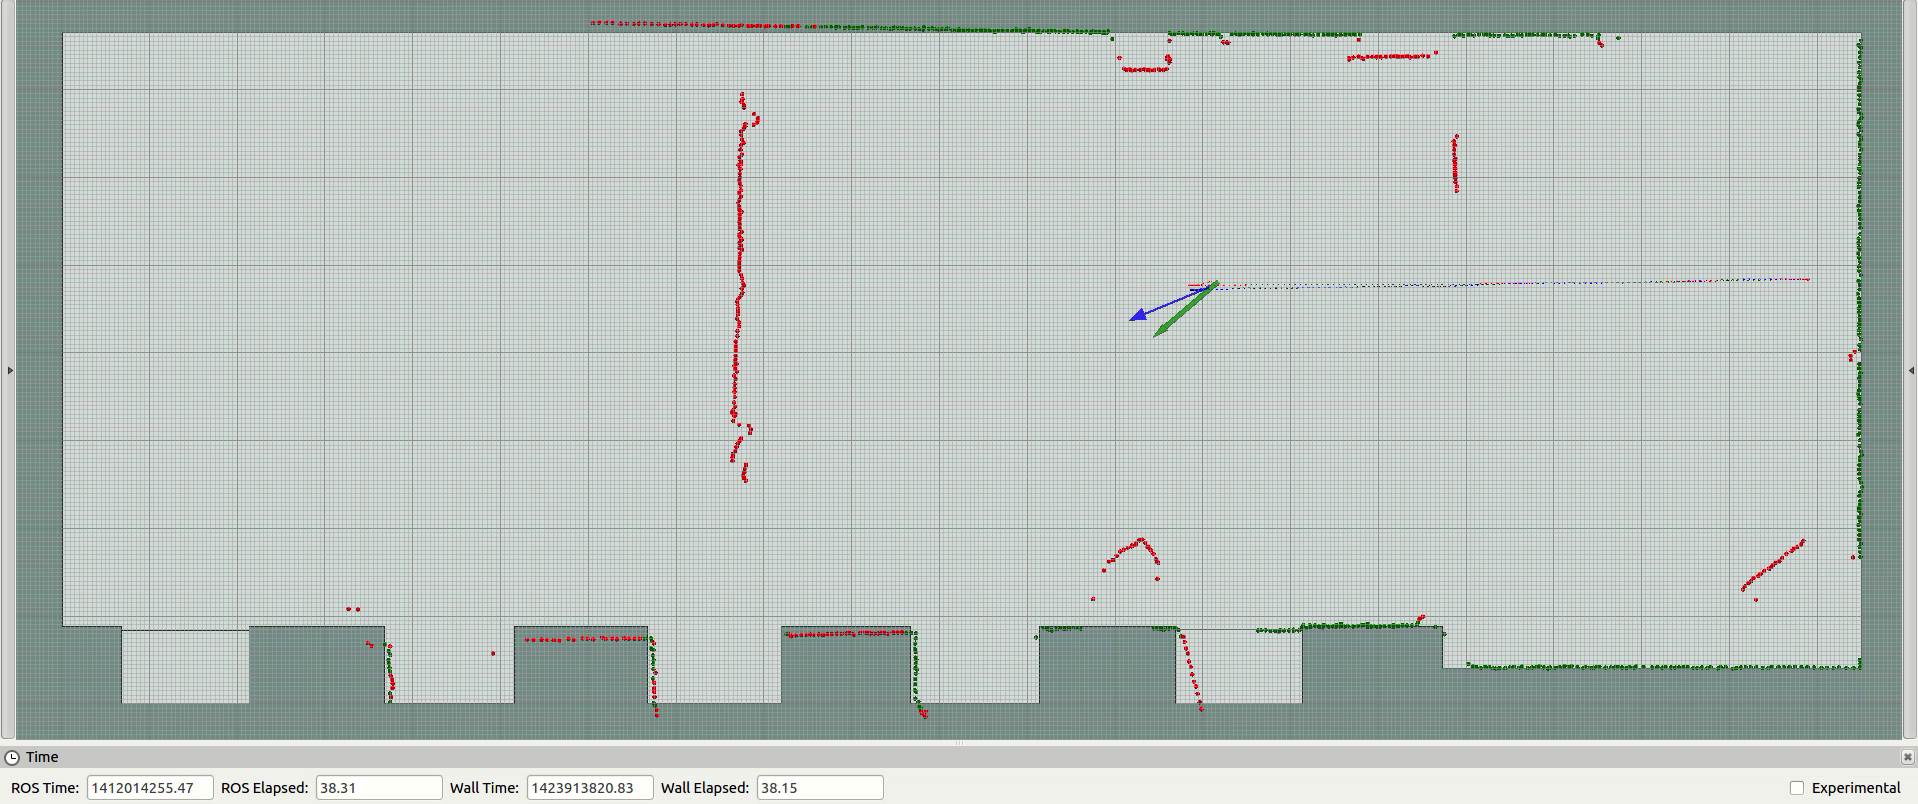
\includegraphics[width=0.97\textwidth]{localization-system-evaluation/tests-3dof/laser-spherical-interpolation/laser-deformation-1}
	\caption{Large laser deformation on opposite walls when the robot is rotating}
	\label{fig:localization-system-evaluation_laser-deformation-1}
\end{figure}

\begin{figure}[H]
	\centering
	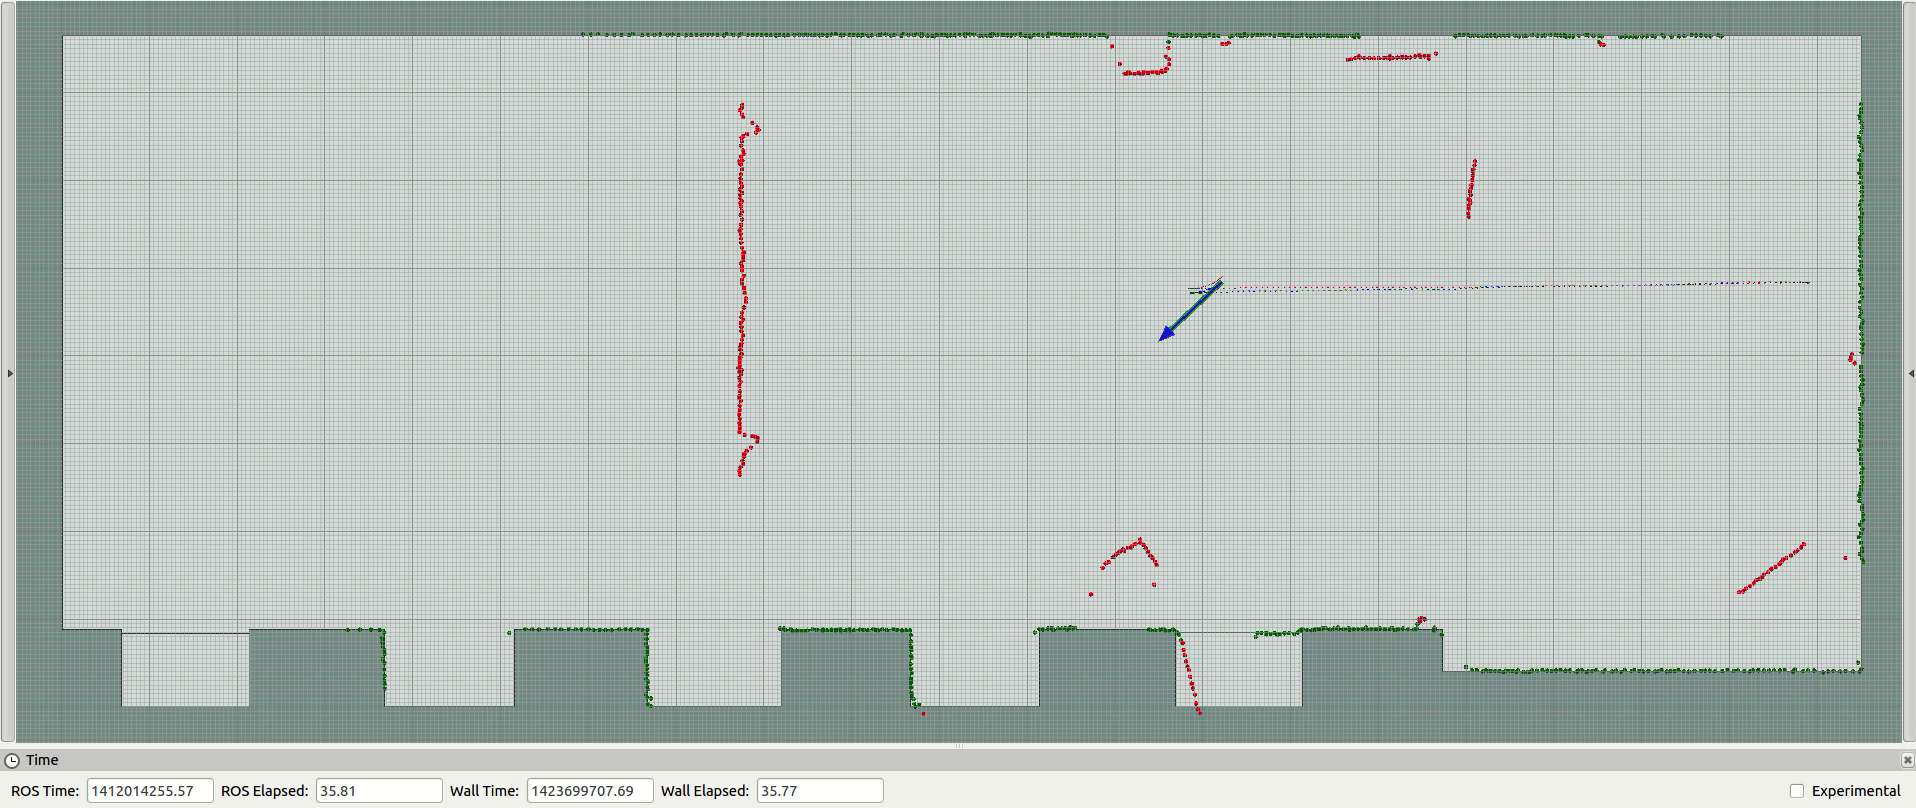
\includegraphics[width=0.97\textwidth]{localization-system-evaluation/tests-3dof/laser-spherical-interpolation/laser-deformation-1-corrected}
	\caption{Correction of the large laser deformation on opposite walls with spherical linear interpolation}
	\label{fig:localization-system-evaluation_laser-deformation-1-corrected}
\end{figure}


\begin{figure}[H]
	\centering
	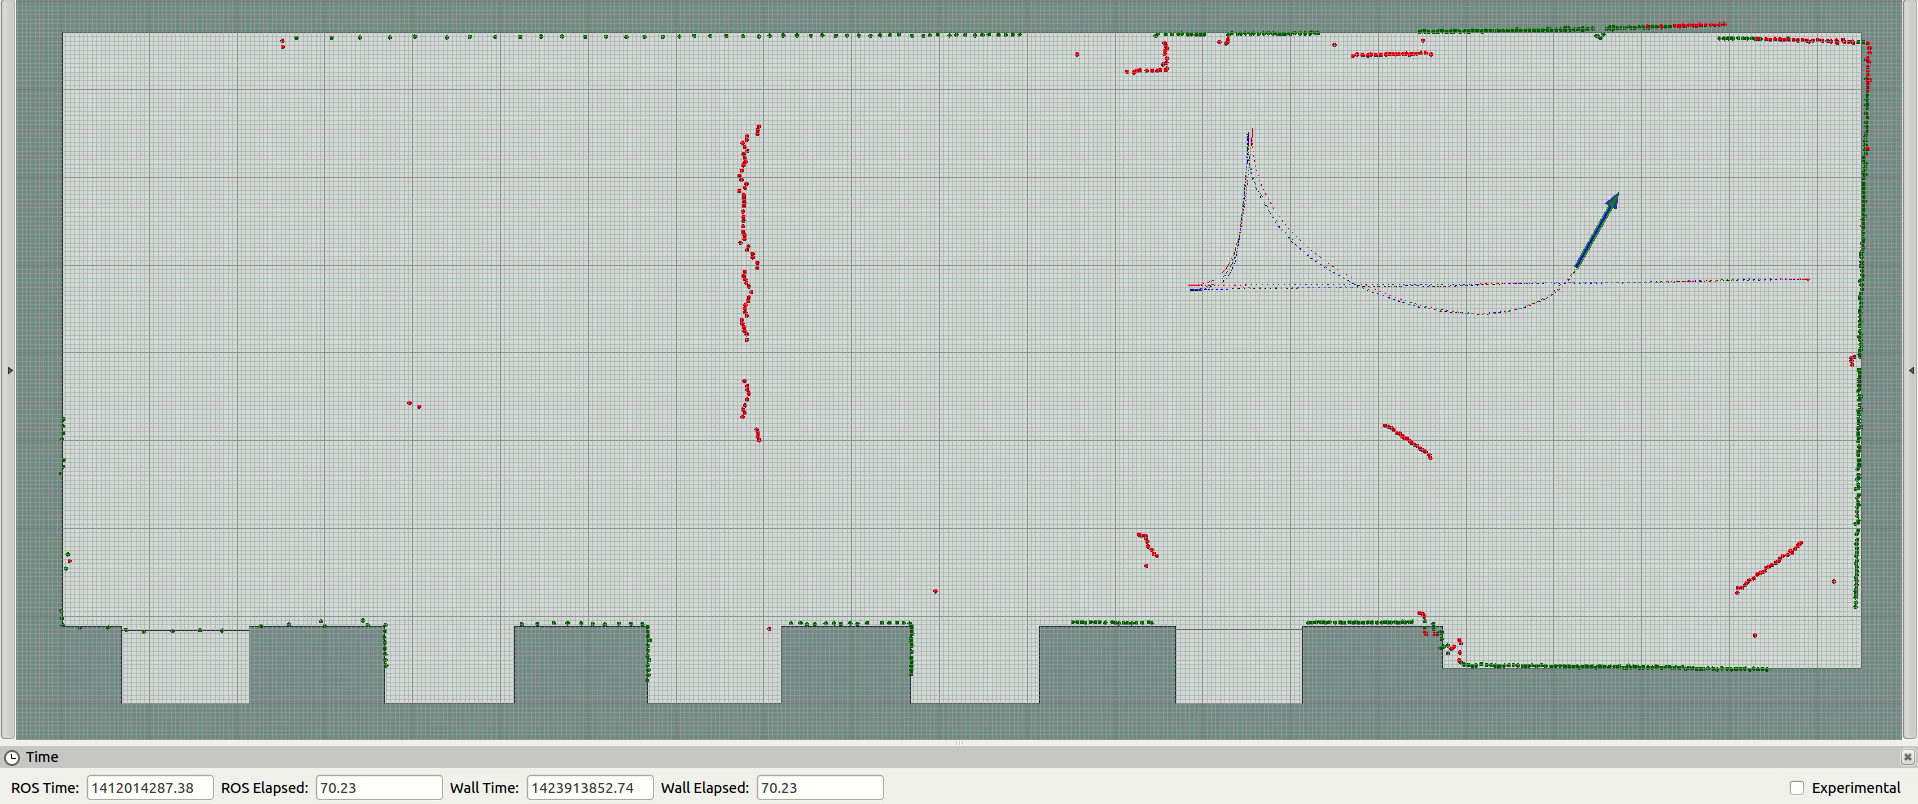
\includegraphics[width=0.97\textwidth]{localization-system-evaluation/tests-3dof/laser-spherical-interpolation/laser-deformation-2}
	\caption{Laser deformation when the robot is rotating}
	\label{fig:localization-system-evaluation_laser-deformation-2}
\end{figure}

\begin{figure}[H]
	\centering
	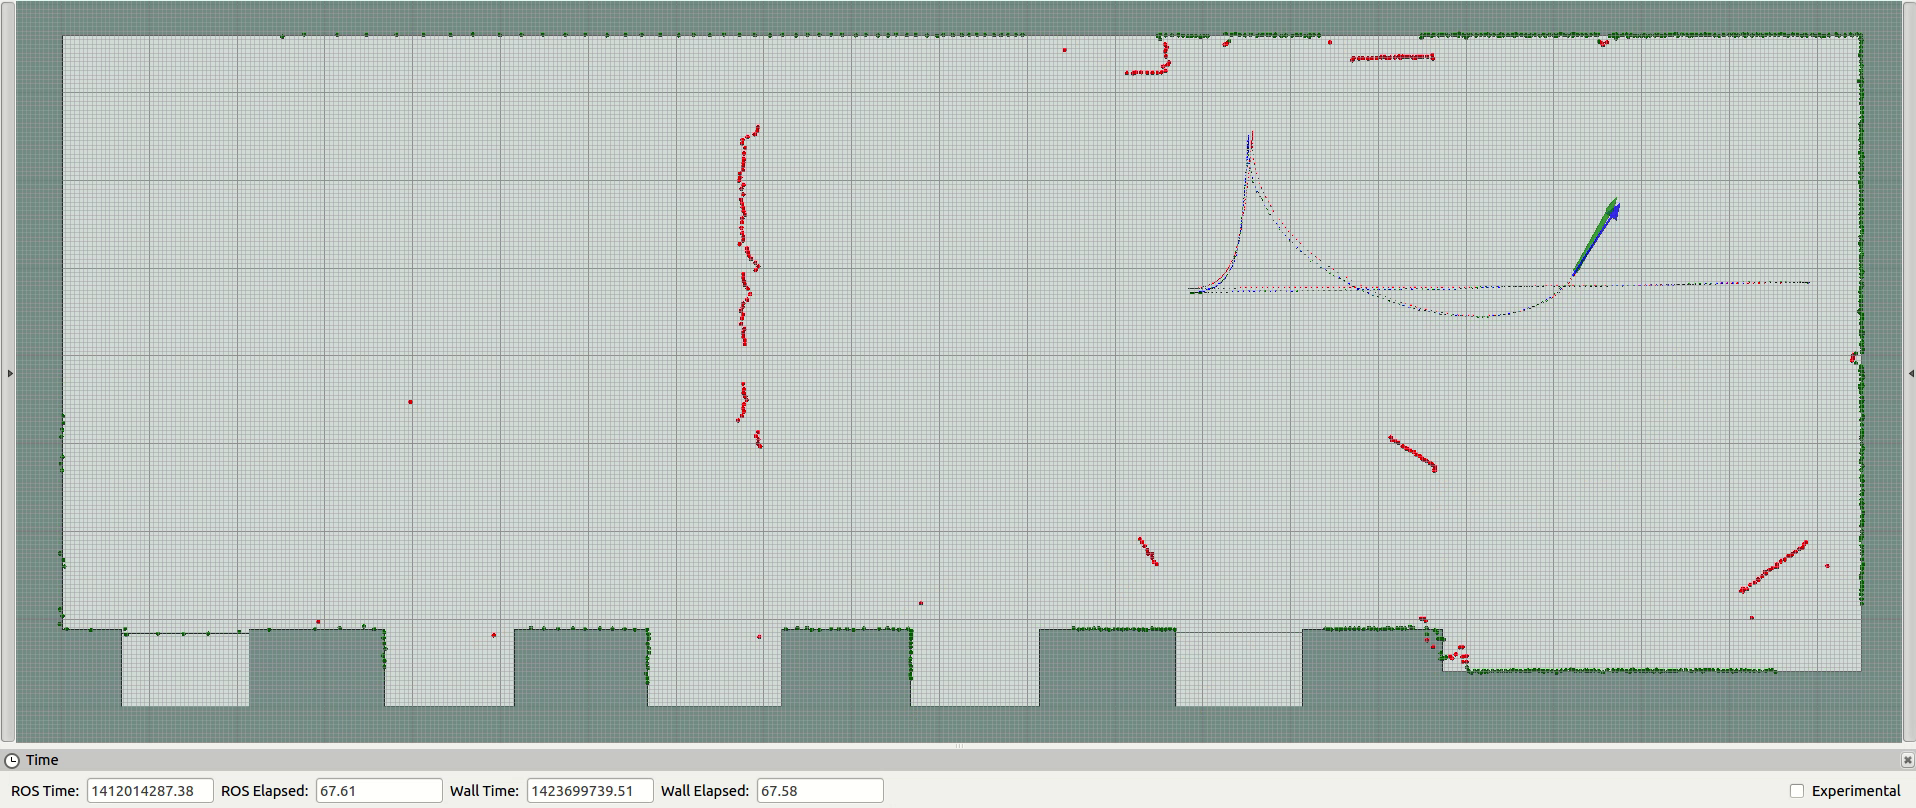
\includegraphics[width=0.97\textwidth]{localization-system-evaluation/tests-3dof/laser-spherical-interpolation/laser-deformation-2-corrected}
	\caption{Correction of the laser deformation with spherical linear interpolation}
	\label{fig:localization-system-evaluation_laser-deformation-2-corrected}
\end{figure}



\subsection{Point cloud preprocessing}

The statistical error of the lasers can be mitigated by merging several laser scans before performing a point cloud registration. This is based on the fact that a considerable amount of laser noise follows a Gaussian distribution, and as such, the effective measurement error can be significantly reduced by retrieving the centroids of a voxel grid applied over the laser data. However, assembling too much laser scans can lead to worse pose tracking if the robot is moving at high speeds, because the lasers would be projected into the map frame with a high position error (because odometry accuracy decreases when the robot speed increases and the localization system will not correct it). As such, the implemented laser assembler supports dynamic reconfiguration of the number of laser scans to assemble (or the period of assembly time) based on the robot estimated velocity. This feature besides improving the pose tracking, it also allows a navigation supervisor to regulate the rate at which the localization system operates. This can be very useful for mobile manipulators because the localization system can have a high update rate when the robot is moving fast and a low update rate when it is moving slower or when it is stopped. This allows a more efficient usage of the platform hardware resources while also improving the localization system accuracy.

Besides reducing the sensor measurement errors, this processing stage also allows the removal of laser shadow points caused by veiling, or small cluster of points that may be associated with temporary objects / people. Moreover, given that the time it takes to perform point cloud registration is proportional to the number of points in the reference and ambient point cloud, voxel / random downsampling can be a very effective technique to adjust the level of detail required (given the computational resources available).



\subsection{\glsentrytext{slam}}

Any self-localization system requires a map to estimate the pose of the robot when using exteroceptive information. If such map doesn't exist, then the first point cloud can be considered as the initial map, and then it can be updated dynamically as new sensor data is processed. This map update approach can use the full registered point cloud or the inliers / outliers only. Full integration is useful when starting a map from scratch (example in \cref{fig:localization-system-evaluation_drl-2.5cm-1.0-bag-speed}). Partial integration can be useful when there is a highly detailed map and we only want to add or remove information from it (examples from \crefrange{fig:localization-system-evaluation_lab-10mm}{fig:localization-system-evaluation_indoor-10mm-dynamic}). Partial integration besides reducing the computational resources required it also allows to keep the detail of the source map, avoiding deformations due to sensor measurement noise. This noise is noticeable in the map in \cref{fig:localization-system-evaluation_lab-10mm-dynamic} (updated with full integration) and was avoided in the map in \cref{fig:localization-system-evaluation_indoor-10mm-dynamic} (updated with outliers only).

Looking at figures from \crefrange{fig:localization-system-evaluation_drl-2.5cm-1.0-bag-speed}{fig:localization-system-evaluation_ground-truth-2.5cm-0.245-time-offset} it can be seen that the proposed localization system was able to achieve equal or even better mapping results than the GMapping\footnote{\url{http://wiki.ros.org/gmapping}} \gls{slam} system and even the ground truth provided by the Raptor-E cameras (that seems to be less suitable for mapping than both the proposed localization system and the GMapping \gls{ros} package).


\begin{figure}[H]
	\centering
	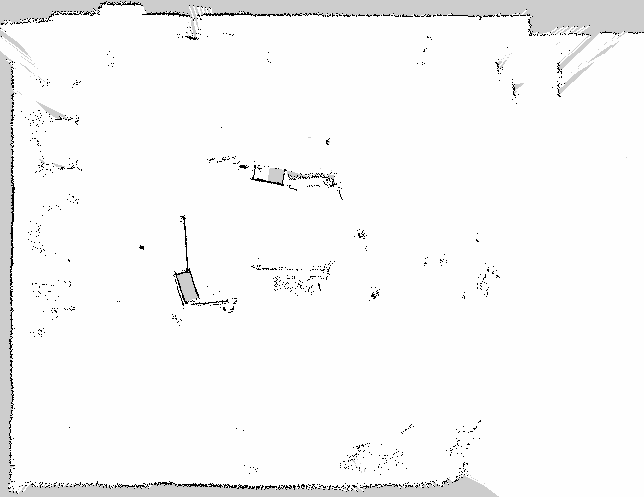
\includegraphics[width=0.53\textwidth]{localization-system-evaluation/tests-3dof/maps/industrial-hall/drl-2.5cm-1.0-bag-speed}
	\caption{Map made with the localization system using full integration in conjunction with OctoMap}
	\label{fig:localization-system-evaluation_drl-2.5cm-1.0-bag-speed}
\end{figure}

\begin{figure}[H]
	\centering
	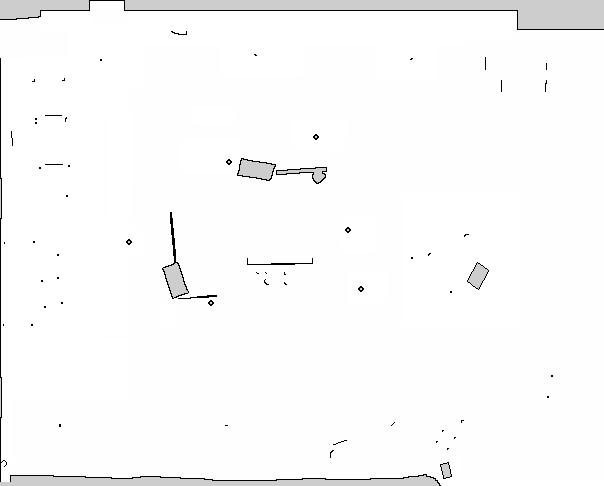
\includegraphics[width=0.53\textwidth]{localization-system-evaluation/tests-3dof/maps/industrial-hall/drl_corrected}
	\caption{Map manually corrected using the previous figure as starting point}
	\label{fig:localization-system-evaluation_drl_corrected}
\end{figure}

\begin{figure}[H]
	\centering
	\includegraphics[width=0.53\textwidth]{localization-system-evaluation/tests-3dof/maps/industrial-hall/gmapping-2.5cm-0.1-bag-speed}
	\caption{Map made with the GMapping package playing the rosbag at 10\% speed}
	\label{fig:localization-system-evaluation_gmapping-2.5cm-0.1-bag-speed}
\end{figure}

\begin{figure}[H]
	\centering
	\includegraphics[width=0.65\textwidth]{localization-system-evaluation/tests-3dof/maps/industrial-hall/gmapping-2.5cm-1.0-bag-speed}
	\caption{Map made with the GMapping package playing the rosbag in real time}
	\label{fig:localization-system-evaluation_gmapping-2.5cm-1.0-bag-speed}
\end{figure}

\begin{figure}[H]
	\centering
	\includegraphics[width=0.65\textwidth]{localization-system-evaluation/tests-3dof/maps/industrial-hall/ground-truth-2.5cm-0.245-time-offset}
	\caption{Map made using the ground truth poses provided by the Raptor-E cameras}
	\label{fig:localization-system-evaluation_ground-truth-2.5cm-0.245-time-offset}
\end{figure}


\begin{figure}[H]
	\centering
	\includegraphics[width=0.7\textwidth]{localization-system-evaluation/tests-3dof/maps/lab-10mm}
	\caption{Original map from room i-108}
	\label{fig:localization-system-evaluation_lab-10mm}
\end{figure}

\begin{figure}[H]
	\centering
	\includegraphics[width=0.7\textwidth]{localization-system-evaluation/tests-3dof/maps/lab-10mm-dynamic}
	\caption{Updated map of room i-108 using full integration}
	\label{fig:localization-system-evaluation_lab-10mm-dynamic}
\end{figure}

\begin{figure}[H]
	\centering
	\includegraphics[width=0.67\textwidth]{localization-system-evaluation/tests-3dof/maps/indoor-10mm}
	\caption{Original map of structured environment}
	\label{fig:localization-system-evaluation_indoor-10mm}
\end{figure}

\begin{figure}[H]
	\centering
	\includegraphics[width=0.67\textwidth]{localization-system-evaluation/tests-3dof/maps/indoor-10mm-dynamic}
	\caption{Updated map of structured environment using partial integration (outliers)}
	\label{fig:localization-system-evaluation_indoor-10mm-dynamic}
\end{figure}



\subsection{Point cloud registration}

Looking at the results present in \cref{app:appendix-a}, such as the laser assembly figures and translation / rotation error graphs from the Jarvis test in the complex path at high velocities (shown from \crefrange{fig:localization-system-evaluation_complex-path-with-outliers-50-30-50-10cm-per-sec-velocity-1-4-scans-drl-cumulative}{fig:localization-system-evaluation_complex-path-with-outliers-50-30-50-10cm-per-sec-velocity-1-4-rotation-error}), it can be seen that the localization system can registered point clouds with much more accuracy than \gls{amcl} (even when using over 5000 particles). The only problems that seem to affect the used algorithms are the point cloud deformation (usually when there is unreliable odometry information, which typically occurs when the robot is moving with high velocities / accelerations), laser measurements errors, unknown objects close to the known reference point cloud and also low resolution maps.

The localization system can tolerate these problems by having a default pipeline configuration for the normal operation of the robot, another for temporary tracking recovery and yet another for initial pose estimation.

The switch between the localization system operation modes using the point cloud registration analysis proved to be a very intuitive and fast process and the overall system configurations seemed to be generic enough to be reused in several types of environments, with different robots equipped with varying types of sensors. Such ease of configuration allows the fast deployment of robots and gives a high confidence that the localization system will remain accurate even in challenging environments. This is not the case with systems such as \gls{amcl}, given that they are very dependent on the odometry and laser models, and as such, require constant retuning when one of these models change.

The ability to switch registration algorithms at runtime based on the quality of the estimated pose proved to be an efficient and flexible architecture choice, since it allowed high precision pose tracking with fast registration algorithms and occasional pose tracking recovery with more robust methods (which happened more often in the tests at higher velocities, in which the odometry was significantly worse).

The initial pose estimation using feature matching was very reliable and successfully found the robot location even in low feature surroundings (as can be seen in \cref{fig:localization-system-evaluation_ship-interior-initial-pose-estimation-sift-fpfh-ransac-gicp,fig:localization-system-evaluation_jarvis-initial-pose-estimation-sift-fpfh-ransac-gicp-1}). Moreover, the output of the accepted initial pose estimations allows the detection of similar map locations by a navigation supervisor, which can then plot a path to disambiguate the initial pose guess and avoid dangerous operations at a wrong position.

\Crefrange{fig:localization-system-evaluation_ship-interior-initial-pose-estimation-sift-fpfh-ransac-gicp}{fig:localization-system-evaluation_jarvis-initial-pose-estimation-sift-fpfh-ransac-gicp-1} show the accepted initial pose estimations using the global localization subsystem presented in \cref{subsec:localization-system_feature-registration}.

The blue circles presented in \cref{fig:localization-system-evaluation_jarvis-initial-pose-estimation-sift-fpfh-ransac-gicp-1} represent the keypoints of the ambient point cloud in the robot start up position, while the violet circles are the reference point cloud keypoints. The green circles are the ambient point cloud laser measurements after performing the initial pose estimation and registration refinement.



\begin{figure}[H]
	\centering
	\includegraphics[width=0.8\textwidth]{appendices/tests-3dof/jarvis-robot/complex-path-with-outliers-50-30-50-10cm-per-sec-velocity-1-4-scans/drl-cumulative}
	\caption{Laser scans assembled on top of the map using the localization system poses}
	\label{fig:localization-system-evaluation_complex-path-with-outliers-50-30-50-10cm-per-sec-velocity-1-4-scans-drl-cumulative}
\end{figure}

\begin{figure}[H]
	\centering
	\includegraphics[width=0.8\textwidth]{appendices/tests-3dof/jarvis-robot/complex-path-with-outliers-50-30-50-10cm-per-sec-velocity-1-4-scans/amcl-cumulative}
	\caption{Laser scans assembled on top of the map using the \glsentrytext{amcl} poses}
	\label{fig:localization-system-evaluation_complex-path-with-outliers-50-30-50-10cm-per-sec-velocity-1-4-scans-amcl-cumulative}
\end{figure}


\begin{figure}[H]
	\centering
	\includegraphics[width=0.87\textwidth]{localization-system-evaluation/tests-3dof/initial_pose_estimation/ship-interior-initial-pose-estimation-sift-fpfh-ransac-gicp}
	\caption{Initial pose estimation using feature matching in Guardian static environment}
	\label{fig:localization-system-evaluation_ship-interior-initial-pose-estimation-sift-fpfh-ransac-gicp}
\end{figure}

\begin{figure}[H]
	\centering
	\includegraphics[width=0.99\textwidth]{localization-system-evaluation/tests-3dof/initial_pose_estimation/jarvis-initial-pose-estimation-sift-fpfh-ransac-gicp-1}
	\caption{Initial pose estimation using feature matching in Jarvis environment}
	\label{fig:localization-system-evaluation_jarvis-initial-pose-estimation-sift-fpfh-ransac-gicp-1}
\end{figure}

\begin{figure}[H]
	\centering
	\includegraphics[width=0.5\textwidth]{localization-system-evaluation/tests-3dof/initial_pose_estimation/jarvis-initial-pose-estimation-sift-fpfh-ransac-gicp-2}
	\caption{Initial pose estimation distribution in Jarvis environment}
	\label{fig:localization-system-evaluation_jarvis-initial-pose-estimation-sift-fpfh-ransac-gicp-2}
\end{figure}




\subsection{Translation and rotation errors}

By analyzing \cref{tab:localization-system-evaluation_3-dof-results,tab:localization-system-evaluation_3-dof-results-odometry-amcl} it can be seen that the proposed 3 \gls{dof} localization system can achieve pose tracking with less than 1 cm in translation error and less than 1 degree in rotation error.

As expected, the tests at lower velocities had less mean error than the ones at higher speeds while requiring slightly less computation time. Also, the tests on the Jarvis robot had more mean error than the corresponding simulator tests. This is due to laser scan deformation that couldn't be simulated and also because the simulators were only able to add Gaussian noise to the laser measurements. To compensate the simulators limitations, the error in odometry and laser measurements in simulation was deliberately higher than the expected values for the physical platforms. This explains why the localization system needed more time to perform the pose estimations in the simulator tests. It can also be seen that adding unknown objects increased the mean error and required computation time while adding dynamic objects increased these values even further (given that a moving object appears in a laser scan as a deformed version of its static shape).

Comparing the results of the tests performed with Jarvis robot  with the tests of the Pioneer robot, it can be seen that even severely reducing the laser range (from 80 to 6 meters), moving the robot in dynamic environments with large occluding objects and even when using a low resolution map (25 mm in the Pioneer tests vs 10 mm in the Jarvis tests), the localization system still managed to track the robot pose with mean translation error (17 mm) bellow the map resolution (25 mm).

These results show that the localization system can reliably achieve high accuracy pose tracking even in dynamic and challenging environments.

\begin{figure}[H]
	\centering
	\begin{minipage}[h]{0.497\textwidth}
		\centering
		\includegraphics[width=0.997\textwidth]{appendices/tests-3dof/jarvis-robot/complex-path-with-outliers-50-30-50-10cm-per-sec-velocity-1-4-scans/graphs/translation-error-millimeters-distributions}
		\caption{Probability distributions for the localization system translation errors}
		\label{fig:localization-system-evaluation_complex-path-with-outliers-50-30-50-10cm-per-sec-velocity-1-4-translation-error}
	\end{minipage}\hfill
	\begin{minipage}[h]{0.497\textwidth}
		\centering
		\includegraphics[width=0.997\textwidth]{appendices/tests-3dof/jarvis-robot/complex-path-with-outliers-50-30-50-10cm-per-sec-velocity-1-4-scans/graphs/rotation-error-degrees-distributions}
		\caption{Probability distributions for the localization system rotation errors}
		\label{fig:localization-system-evaluation_complex-path-with-outliers-50-30-50-10cm-per-sec-velocity-1-4-rotation-error}
	\end{minipage}
\end{figure}


\subsection{Computation time}

Looking at the computation time graphs in \cref{fig:localization-system-evaluation_complex-path-with-outliers-50-30-50-10cm-per-sec-velocity-1-4-global-computation-time-distributions,tab:localization-system-evaluation_3-dof-results} and \cref{app:appendix-a} it can be seen that the localization system can register the point clouds very fast (between 5 and 30 milliseconds), which is more than enough to process all the incoming laser scans in real time (typically \glspl{lidar} generate scans every 100 milliseconds). Moreover, the computation time seems to be very stable, with occasional peaks due to laser deformation or varying percentage of outliers.

The global computation time is mostly associated with the point cloud registration stage, while the rest of it is due to normal estimation and point cloud preprocessing algorithms.

\begin{figure}[H]
	\centering
	\includegraphics[width=0.63\textwidth]{appendices/tests-3dof/jarvis-robot/complex-path-with-outliers-50-30-50-10cm-per-sec-velocity-1-4-scans/graphs/computation-times-milliseconds-global-time-distributions}
	\caption{Probability distributions for the localization system computation time}
	\label{fig:localization-system-evaluation_complex-path-with-outliers-50-30-50-10cm-per-sec-velocity-1-4-global-computation-time-distributions}
\end{figure}



\clearpage

\section{6 \glsentrytext{dof} localization system tests}

\subsection{Overview}

The main 6 \gls{dof} results retrieved with the localization system are shown in \cref{tab:localization-system-evaluation_6-dof-results} and \cref{app:appendix-b}. The first two experiments were done to evaluate the accuracy of the point cloud registration algorithms while the last one aimed to test the robustness against temporary absence of valid sensor data (in this test the Kinect had periods in which most of its field of view was outside the map).

These tests were retrieved with a known initial pose and used \gls{icp} point-to-point as tracking algorithm and \gls{icp} point-to-plane as tracking recovery method. The 3D map was done with the localization system in \gls{slam} mode and used continuous surface reconstruction in order to create an accurate representation of the environment and reduce the impact of the measurements noise. This map was later downsampled using a voxel grid with 20 mm cells in order to allow real-time processing of the Kinect data.

The next sections will provide an analysis of the 6 \gls{dof} results achieved with the proposed localization system (shown in \cref{app:appendix-b}). It will start by explaining the importance of point cloud processing and how it helps reduce the cloud registration time. Then it will give an overview of the 3D map building capabilities and it will finished with an analysis of the translation and rotation errors along with the computation time.


\begin{sidewaystable}
	\caption{6 \glsentrytext{dof} results}
	\tabulinesep = 1.2ex
	\setlength{\tabcolsep}{0.2em}
	\centering
	\tiny
	\begin{tabu} to \textwidth { X[m,c] X[m,c] X[1.7m,c] X[m,c] X[0.01m,c] X[m,c] X[m,c] X[0.01m,c] X[m,c] X[m,c] X[0.01m,c] X[m,c] X[m,c] X[0.01m,c] X[m,c] X[m,c] }
		\hline
		\multicolumn{4}{c}{Test conditions} && \multicolumn{2}{c}{Translation error (millimeters)} && \multicolumn{2}{c}{Rotation error (degrees)} && \multicolumn{2}{c}{Outliers percentage [0..100]} && \multicolumn{2}{c}{Global computation time (milliseconds)} \\
		\cline{1-4} \cline{6-7} \cline{9-10} \cline{12-13} \cline{15-16}
		Section 	& Path shape 											& Path velocities 		& Map cell resolution 	&& Mean   	& Standard deviation 	&& Mean  	& Standard deviation 	&& Mean  	& Standard deviation 	&& Mean   & Standard deviation  \\ \hline
		B.1.1		& Overview fly											& 30 cm/s				& 20 mm					&& 17.926	& 9.789					&& 3.027 	& 0.638					&& 0.165	& 0.172					&& 30.714 &	11.407				\\
		B.1.2		& Mainly translations									& 20 cm/s				& 20 mm					&& 14.162	& 7.990					&& 2.486 	& 0.975					&& 0.983	& 1.874					&& 32.296 &	10.757				\\
		B.1.3		& Mainly rotations										& 10 cm/s				& 20 mm					&& 16.576	& 9.389					&& 2.738 	& 0.583					&& 1.214	& 3.148					&& 29.818 &	9.134				\\
		\hline
	\end{tabu}
	\label{tab:localization-system-evaluation_6-dof-results}
\end{sidewaystable}


\subsection{Point cloud preprocessing}

Point cloud preprocessing can have a very significant role when performing 6 \gls{dof} cloud registration for self-localization. This is due to real-time requirements and also because the computation time increases substantially when registering large point clouds. One way to control this problem is by preprocessing the point cloud with a voxel grid to adjust the level of detail and also assign a limit to the number of points that come from sensors. This can be achieved with random sampling or similar point selection techniques, as can be seen in \cref{fig:localization-system-evaluation_kinect-fly-30cm-per-sec-velocity-drl-filters} (filtered cloud has larger points than the reference cloud). Moreover, depending on the sensor used, it may be wise to restrict the points to a given range, and discard the rest that are too far way (given that these measurements will have more errors).

\begin{figure}[H]
	\centering
	\includegraphics[width=0.45\textwidth]{localization-system-evaluation/tests-6dof/kinect-fly-30cm-per-sec-velocity/drl}
	\caption{Example of filtered point cloud from Kinect data}
	\label{fig:localization-system-evaluation_kinect-fly-30cm-per-sec-velocity-drl-filters}
\end{figure}


\subsection{\glsentrytext{slam}}

The proposed localization system can perform mapping of the environment and is able to build very detailed point clouds. These point clouds can be continuously re-sampled with the Moving Least Squares algorithm (example in \cref{fig:localization-system-evaluation_kinect-fly-30cm-per-sec-velocity-drl-slam}) in order to reconstruct the surfaces of the environment and attenuate the double wall effects and high sensor noise.

The localization system can also dynamic update the 3D map in order to remove missing objects from the reference point cloud and also add new ones.

\begin{figure}[H]
	\centering
	\begin{subfigure}[ht]{0.55\textwidth}
		\centering
		\includegraphics[width=\textwidth]{localization-system-evaluation/tests-6dof/kinect-fly-30cm-per-sec-velocity/3d-slam-1-gt}
	\end{subfigure}
	\begin{subfigure}[ht]{0.55\textwidth}
		\centering
		\includegraphics[width=\textwidth]{localization-system-evaluation/tests-6dof/kinect-fly-30cm-per-sec-velocity/3d-slam-2-gt}
	\end{subfigure}
	\begin{subfigure}[ht]{0.55\textwidth}
		\centering
		\includegraphics[width=\textwidth]{localization-system-evaluation/tests-6dof/kinect-fly-30cm-per-sec-velocity/3d-slam-3-gt}
	\end{subfigure}
	\begin{subfigure}[ht]{0.55\textwidth}
		\centering
		\includegraphics[width=\textwidth]{localization-system-evaluation/tests-6dof/kinect-fly-30cm-per-sec-velocity/3d-slam-4-gt}
	\end{subfigure}
	\caption{3D SLAM using the ground truth poses}
	\label{fig:localization-system-evaluation_kinect-fly-30cm-per-sec-velocity-gt-slam}
\end{figure}

\begin{figure}[H]
	\centering
	\begin{subfigure}[ht]{0.75\textwidth}
		\centering
		\includegraphics[width=\textwidth]{localization-system-evaluation/tests-6dof/kinect-fly-30cm-per-sec-velocity/3d-slam-1}
	\end{subfigure}
	\begin{subfigure}[ht]{0.75\textwidth}
		\centering
		\includegraphics[width=\textwidth]{localization-system-evaluation/tests-6dof/kinect-fly-30cm-per-sec-velocity/3d-slam-2}
	\end{subfigure}
	\begin{subfigure}[ht]{0.75\textwidth}
		\centering
		\includegraphics[width=\textwidth]{localization-system-evaluation/tests-6dof/kinect-fly-30cm-per-sec-velocity/3d-slam-3}
	\end{subfigure}
	\begin{subfigure}[ht]{0.75\textwidth}
		\centering
		\includegraphics[width=\textwidth]{localization-system-evaluation/tests-6dof/kinect-fly-30cm-per-sec-velocity/3d-slam-4}
	\end{subfigure}
	\caption{3D SLAM using the localization system with surface reconstruction}
	\label{fig:localization-system-evaluation_kinect-fly-30cm-per-sec-velocity-drl-slam}
\end{figure}


\subsection{Point cloud registration}

Looking at the animated figures in \cref{app:appendix-b} and the assembly of the registered point clouds (shown in \cref{fig:localization-system-evaluation_kinect-fly-30cm-per-sec-velocity-drl-cumulative}), it is clear that the proposed localization system is able to register point clouds with high accuracy, even when they are severely downsampled (due to real-time processing constraints). Moreover, the localization system is robust against temporary absence of sensor data (when the field of view of the Kinect was outside the known map) and was able to quickly recover to accurate tracking when valid sensor data was given. In these situations the recovery algorithms were activated, switching the registration algorithm from \gls{icp} point-to-point to \gls{icp} point-to-plane. Given that these sensor data outages were temporary, the initial pose algorithms weren't necessary. Nevertheless, if the Kinect remained outside the map for a longer period of time, the localization system would alert that the tracking was lost and it would try to find its current pose using feature matching.

Comparing \cref{fig:localization-system-evaluation_kinect_translation_path-a} and \cref{fig:localization-system-evaluation_kinect_translation_path-b}, it can be seen that the proposed localization system achieved better pose tracking than the \emph{ethzasl\_icp\_mapper} \gls{ros} package \cite{Pomerleau2011} (authors of this Kinect dataset). Moreover, the \gls{slam} map shown in \cref{fig:localization-system-evaluation_kinect-fly-30cm-per-sec-velocity-drl-slam} seems to have better quality than the map generated using the ground truth poses (shown in \cref{fig:localization-system-evaluation_kinect-fly-30cm-per-sec-velocity-gt-slam,fig:localization-system-evaluation_kinect-fly-30cm-per-sec-velocity-gt-cumulative}).

\begin{figure}[H]
	\centering
	\begin{minipage}[b]{0.49\textwidth}
		\centering
		\includegraphics[width=0.97\textwidth]{localization-system-evaluation/tests-6dof/kinect-fly-30cm-per-sec-velocity/robot-movement-path}
		\caption{Poses estimated by the ground truth and localization system}
		\label{fig:localization-system-evaluation_kinect_translation_path-a}
	\end{minipage}\hfill
	\begin{minipage}[b]{0.49\textwidth}
		\centering
		\includegraphics[width=0.8\textwidth]{localization-system-evaluation/tests-6dof/kinect-fly-30cm-per-sec-velocity/ethzasl-icp-mapping-path}
		\caption{Poses estimated by the \emph{ethzasl\_icp\_mapper} \glsentrytext{ros} package \cite{Pomerleau2011}}
		\label{fig:localization-system-evaluation_kinect_translation_path-b}
	\end{minipage}
\end{figure}

\begin{figure}[H]
	\centering
	\includegraphics[width=0.75\textwidth]{localization-system-evaluation/tests-6dof/kinect-fly-30cm-per-sec-velocity/drl-cumulative}
	\caption{Point clouds assembled on top of the map using the localization system poses (for the top part of the figure: green arrows $\rightarrow$ ground truth poses, red arrows $\rightarrow$ localization system poses)}
	\label{fig:localization-system-evaluation_kinect-fly-30cm-per-sec-velocity-drl-cumulative}
\end{figure}

\begin{figure}[H]
	\centering
	\includegraphics[width=0.75\textwidth]{localization-system-evaluation/tests-6dof/kinect-fly-30cm-per-sec-velocity/ground-truth-cumulative}
	\caption{Point clouds assembled on top of the map using the ground truth poses}
	\label{fig:localization-system-evaluation_kinect-fly-30cm-per-sec-velocity-gt-cumulative}
\end{figure}



\subsection{Translation and rotation errors}

The results presented in \cref{tab:localization-system-evaluation_6-dof-results,app:appendix-b} and in \cref{fig:localization-system-evaluation_kinect-fly-30cm-per-sec-velocity-translation-error,fig:localization-system-evaluation_kinect-fly-30cm-per-sec-velocity-rotation-error}, shown that the localization system can maintain high accuracy pose tracking, with translation error bellow two centimeters and rotation error around 3 degrees when good sensor data is available. Moreover it can quickly recover from temporary registration problems caused by occlusions or accelerations.

\Cref{fig:localization-system-evaluation_kinect_translation_path-a,fig:localization-system-evaluation_kinect_translation_path-b} also shows that the proposed localization system achieved less overall translation error than the tracking system proposed by the authors of this Kinect dataset \cite{Pomerleau2011}.

\begin{figure}[H]
	\centering
	\includegraphics[width=0.57\textwidth]{localization-system-evaluation/tests-6dof/kinect-fly-30cm-per-sec-velocity/translation-error-millimeters-distributions}
	\caption{Probability distributions for the localization system translation errors}
	\label{fig:localization-system-evaluation_kinect-fly-30cm-per-sec-velocity-translation-error}
\end{figure}

\begin{figure}[H]
	\centering
	\includegraphics[width=0.57\textwidth]{localization-system-evaluation/tests-6dof/kinect-fly-30cm-per-sec-velocity/rotation-error-degrees-distributions}
	\caption{Probability distributions for the localization system rotation errors}
	\label{fig:localization-system-evaluation_kinect-fly-30cm-per-sec-velocity-rotation-error}
\end{figure}



\subsection{Computation time}

The localization system was able to achieve a mean computation time low enough to allow real time processing of the Kinect point cloud sensor data (shown in \cref{fig:localization-system-evaluation_kinect-fly-30cm-per-sec-velocity-computation-time}). Depending on the accuracy requirements, the computation time can be lowered even further by tuning the preprocessing filters described in \cref{fig:localization_system_filtering-and-down-sampling}, in order to reduce the number of points used in the cloud registration.

\begin{figure}[H]
	\centering
	\includegraphics[width=0.57\textwidth]{localization-system-evaluation/tests-6dof/kinect-fly-30cm-per-sec-velocity/computation-times-milliseconds-global-time-distributions}
	\caption{Probability distributions for the localization system global computation time}
	\label{fig:localization-system-evaluation_kinect-fly-30cm-per-sec-velocity-computation-time}
\end{figure}

\chapter{Conclusions} \label{chap:conclusions-and-future-work}



\section*{}

The proposed localization system is able to maintain pose tracking with less 1-2 centimeters of translation error and less than a 1-3 degrees of rotation error (in 3 and 6 DoF respectively) with the sensors moving at several velocities even in cluttered and dynamic environments. Moreover, when tracking is lost or no initial pose is given, the system is able to find a valid global pose estimate by switching to more robust registration algorithms that use feature matching. This approach achieved fast pose tracking and reliable initial pose estimation while also providing the set of the accepted initial poses before registration refinement, which can be very valuable information for a navigation supervisor when the robot is in an ambiguous region that can be registered in similar zones of the known map. The system also allows dynamic reconfiguration of the number of laser scans to assemble in order to mitigate laser measurement errors and can adapt its rate of operation according to the robot estimated velocity.

The sub-centimeter accuracy achieved by the proposed localization system along with the dynamic map update capability and the need of no artificial landmarks / ambient modifications will allow the fast deployment of mobile robots capable to operate safely and accurately in cluttered environments.



\section{Main contributions}

The following list gives an overview of the main contributions of the presented work:

\begin{itemize}
	\item A \gls{lidar} assembler\footnote{\url{https://github.com/carlosmccosta/laserscan_to_pointcloud}} capable of:
	\begin{itemize}
		\item Merging measurements from several sensors
		\item Dynamic adjust its configurations based on the speed of the robot in order to merge more scans when the robot is moving slower
		\item Use spherical linear interpolation to reduce scan deformation
		\item Emulate a 3D sensor when the \gls{lidar} is mounted on a tilting platform
	\end{itemize}

	\item An localization system\footnote{\url{https://github.com/carlosmccosta/dynamic_robot_localization}} that:
	\begin{itemize}
		\item Is efficient, modular and extensible to new 3/6 \gls{dof} algorithms
		\item Can dynamically and incrementally update the localization map
		\item Provides the set of acceptable initial poses when reseting tracking (useful for localization supervisors)
		\item Gives several localization quality metrics such as percentage, \gls{rmse} and angular distribution of the correctly registered points
		\item Gives the possibility to use 3 different point cloud registration algorithms based on the tracking state (normal tracking, tracking recovery, initial pose estimation)
	\end{itemize}

	\item Development of a testing infrastructure to automate the collection, analysis and generation of localization results

	\item 3 \gls{dof} Localization datasets\footnote{\url{https://github.com/carlosmccosta/dynamic_robot_localization_tests}}:
	\begin{itemize}
		\item 4 datasets with subcentimeter ground truth in static and dynamic environments using a robot moving at different speeds
		\item 6 Gazebo and 6 Stage simulation datasets
		\item Improvement of external 3/6 \gls{dof} datasets (ground truth time synchronization and laser transformations calibration)
	\end{itemize}

	\item Test of the localization system on public datasets and comparison with:
	\begin{itemize}
		\item Ground truth systems from three different testing environments
		\item Widely used localization systems (\gls{amcl} and ethzasl-icp-mapper)
		\item Well known \gls{slam} system (GMapping)
	\end{itemize}
 	
	\item In the context of the \gls{carlos} project:
	\begin{itemize}
		\item The robot hardware configuration proved adequate for the intended tasks and environment
		\item The 3 \gls{dof} localization system was able to run in real time on the low computational power on-board computer
	\end{itemize}
\end{itemize}



\section{Future work}

The current implementation of the self-localization system can be further improved with \gls{gpu} support \cite{Tamaki2010} in order to achieve higher update rates in 6 \gls{dof} and also with loop closing algorithms \cite{Grisetti2012} in order to become a complete \gls{slam} system and allow the creation of accurate maps of very large environments. Moreover, it could be extended to support image based localization \cite{Labb2014} and semantic perception and mapping of the environment \cite{Santos2013}.





%---------------------------------------------------------------------------------------------------
% Appendixes, bibliography and index
%---------------------------------------------------------------------------------------------------

\appendix
\chapter{Appendix 1} \label{app:appendix1}



\section*{}

FF



\section{FF}

FF


\PrintBib{references/references}
%\PrintIndex


\end{document}
